\documentclass[twocolumn, letterpaper]{article}
\raggedbottom
\usepackage[margin=1in]{geometry}
\usepackage{listings}
\usepackage{titlesec}
\usepackage{graphicx}
\usepackage{amsfonts}
\usepackage{amsmath}
\usepackage{float}
\usepackage{xcolor}
\usepackage{booktabs}
\usepackage{relsize}
\newcommand*{\ditto}{\texttt{"}}
\usepackage{bbm}
\usepackage{array}
\usepackage{hyperref}
\usepackage[nameinlink,noabbrev]{cleveref}
\usepackage{dblfloatfix}
\usepackage{natbib}
\setcounter{secnumdepth}{5}
\setcounter{tocdepth}{5}
\usepackage{XCharter}
\usepackage[charter]{newtxmath}
\definecolor{codegreen}{rgb}{0,0.6,0}
\definecolor{codegray}{rgb}{0.5,0.5,0.5}
\definecolor{codepurple}{rgb}{0.58,0,0.82}
\definecolor{backcolour}{rgb}{0.95,0.95,0.92}

\lstdefinestyle{mystyle}{
    backgroundcolor=\color{backcolour},   
    commentstyle=\color{codegreen},
    keywordstyle=\color{magenta},
    numberstyle=\tiny\color{codegray},
    stringstyle=\color{codepurple},
    basicstyle=\ttfamily\footnotesize,
    breakatwhitespace=false,         
    breaklines=true,                 
    captionpos=b,                    
    keepspaces=true,                 
    numbers=left,                    
    numbersep=5pt,                  
    showspaces=false,                
    showstringspaces=false,
    showtabs=false,                  
    tabsize=2
}

\lstset{style=mystyle}
\newcommand{\panel}[1]{\textbf{\MakeUppercase{#1}.}}

\titleformat{\paragraph}
  {\normalfont\normalsize\bfseries}
  {\theparagraph}{1em}{}

\titlespacing*{\paragraph}
{0pt}{3.25ex plus 1ex minus .2ex}{1.5ex plus .2ex}
\setlength{\textfloatsep}{10pt plus 2pt minus 2pt}
\setlength{\floatsep}{8pt plus 2pt minus 2pt} 
\setlength{\intextsep}{10pt plus 2pt minus 2pt}
\setlength{\dbltextfloatsep}{10pt plus 2pt minus 2pt}
\setlength{\dblfloatsep}{8pt plus 2pt minus 2pt}

\titleformat{\subparagraph}
  {\normalfont\small\bfseries}
  {\thesubparagraph}{1em}{}

\titlespacing*{\subparagraph}
  {0pt}{3ex plus 1ex minus .2ex}{1ex plus .2ex}

\title{Self-excitation: Everyone Does It\\[0.5em]
  \large\textit{Self-exciting hurdled autoregressive models as a new approach to scientific productivity.}}
\author{Samantha Magid \& Sam Zhang}

\begin{document}
\maketitle
\begin{center}
\large{\textbf{Abstract}}
\end{center}

\begin{quote}
Iterative testing and improvement in the field of geometric random walks and autoregressive models as approximations to generators of scientific productivity trajectories converged to an unsatisfactory apex marked by repeated failure modes and shortfalls. We then identified issues with the GRW in the follow-up draft to \textit{Scientific Productivity as a Random Walk} that weakened the justifications for its use and led us to move to other models. Further, statistical tests of empirical data demonstrated that current productivity is insufficient as a first-order Markov state to predict future productivity. These findings motivated development in a novel direction of scholar-agnostic model architecture. We identify a simple self-exciting hurdled model that shows a stronger fit across various metrics and supports the original claim in \textit{Scientific Productivity as a Random Walk} that temporal stochastic processes better reproduce scientific productivity trajectories than William Shockley's fixed talent/men-of-merit model \citep{zhangrandomwalk, shockley1957}. We conclude that our design is entirely in line with the theoretical spirit of the follow-up draft and substantially improves on structural shortcomings of our tested GRWs and ARs.
\end{quote}

\noindent\textbf{Keywords:}
scientific productivity; self-exciting processes; hurdle models;
path dependence; career dynamics; Markov sufficiency;
cumulative advantage; rank persistence

\noindent\textbf{Code:}
\href{https://github.com/crabwife/spaarw_followup}{GitHub}

\section{Introduction}
\label{sec:introduction}
Previously developed and tested geometric, autoregressive, and hurdle models reproduced some marginal and moment-based successes but always lost empirical rank persistence. Increasing autoregressive order and adding specialized dropout and restart gadgets marginally improved local diagnostics without fixing this failure. Additionally, while we had moved away from the GRW proposed by the draft due to poor experimental results, upon revisiting it, we found mathematical and implementation errors severe enough to both discourage the draft GRWs as explanatory candidates and to weaken many of the conclusions in the draft (see \Cref{supp:grw_explode} and \Cref{supp:bugs} for more information).

This motivated an alternative model in which earlier productivity enters through a compressed, decaying history state.

Further motivating the addition of a compressed history state were the results of Markov sufficiency testing on $q_t$. We found that $q_t$ alone is insufficient as a first-order Markov state for productivity, and when it is used as one, it especially misrepresents persistence at the high and low extremes. 

This dynamic was recognized in \textit{Scientific Productivity as a Random Walk}. The CK test results described in \Cref{emp_motivation:ck_qt} further reject the sufficiency of $q_t$ as a first-order state as it has been used, and support the need to model beyond it. 

The GRW hypothesis could be understood as
\begin{center}
    $q_t$ compounds multiplicatively.
\end{center}
Our new hypothesis, now that we've found history has predictive value and GRWs struggle to perform, is that
\begin{center}
    past $q$ affects a persistent memory state.
\end{center}
To rigorously support this hypothesis, we performed several statistical tests with the empirical data and with unrestricted first-order models. 

\section{Empirical Motivation}
\label{sec:empirical_motivation}
\begin{figure*}[!b]
    \centering
    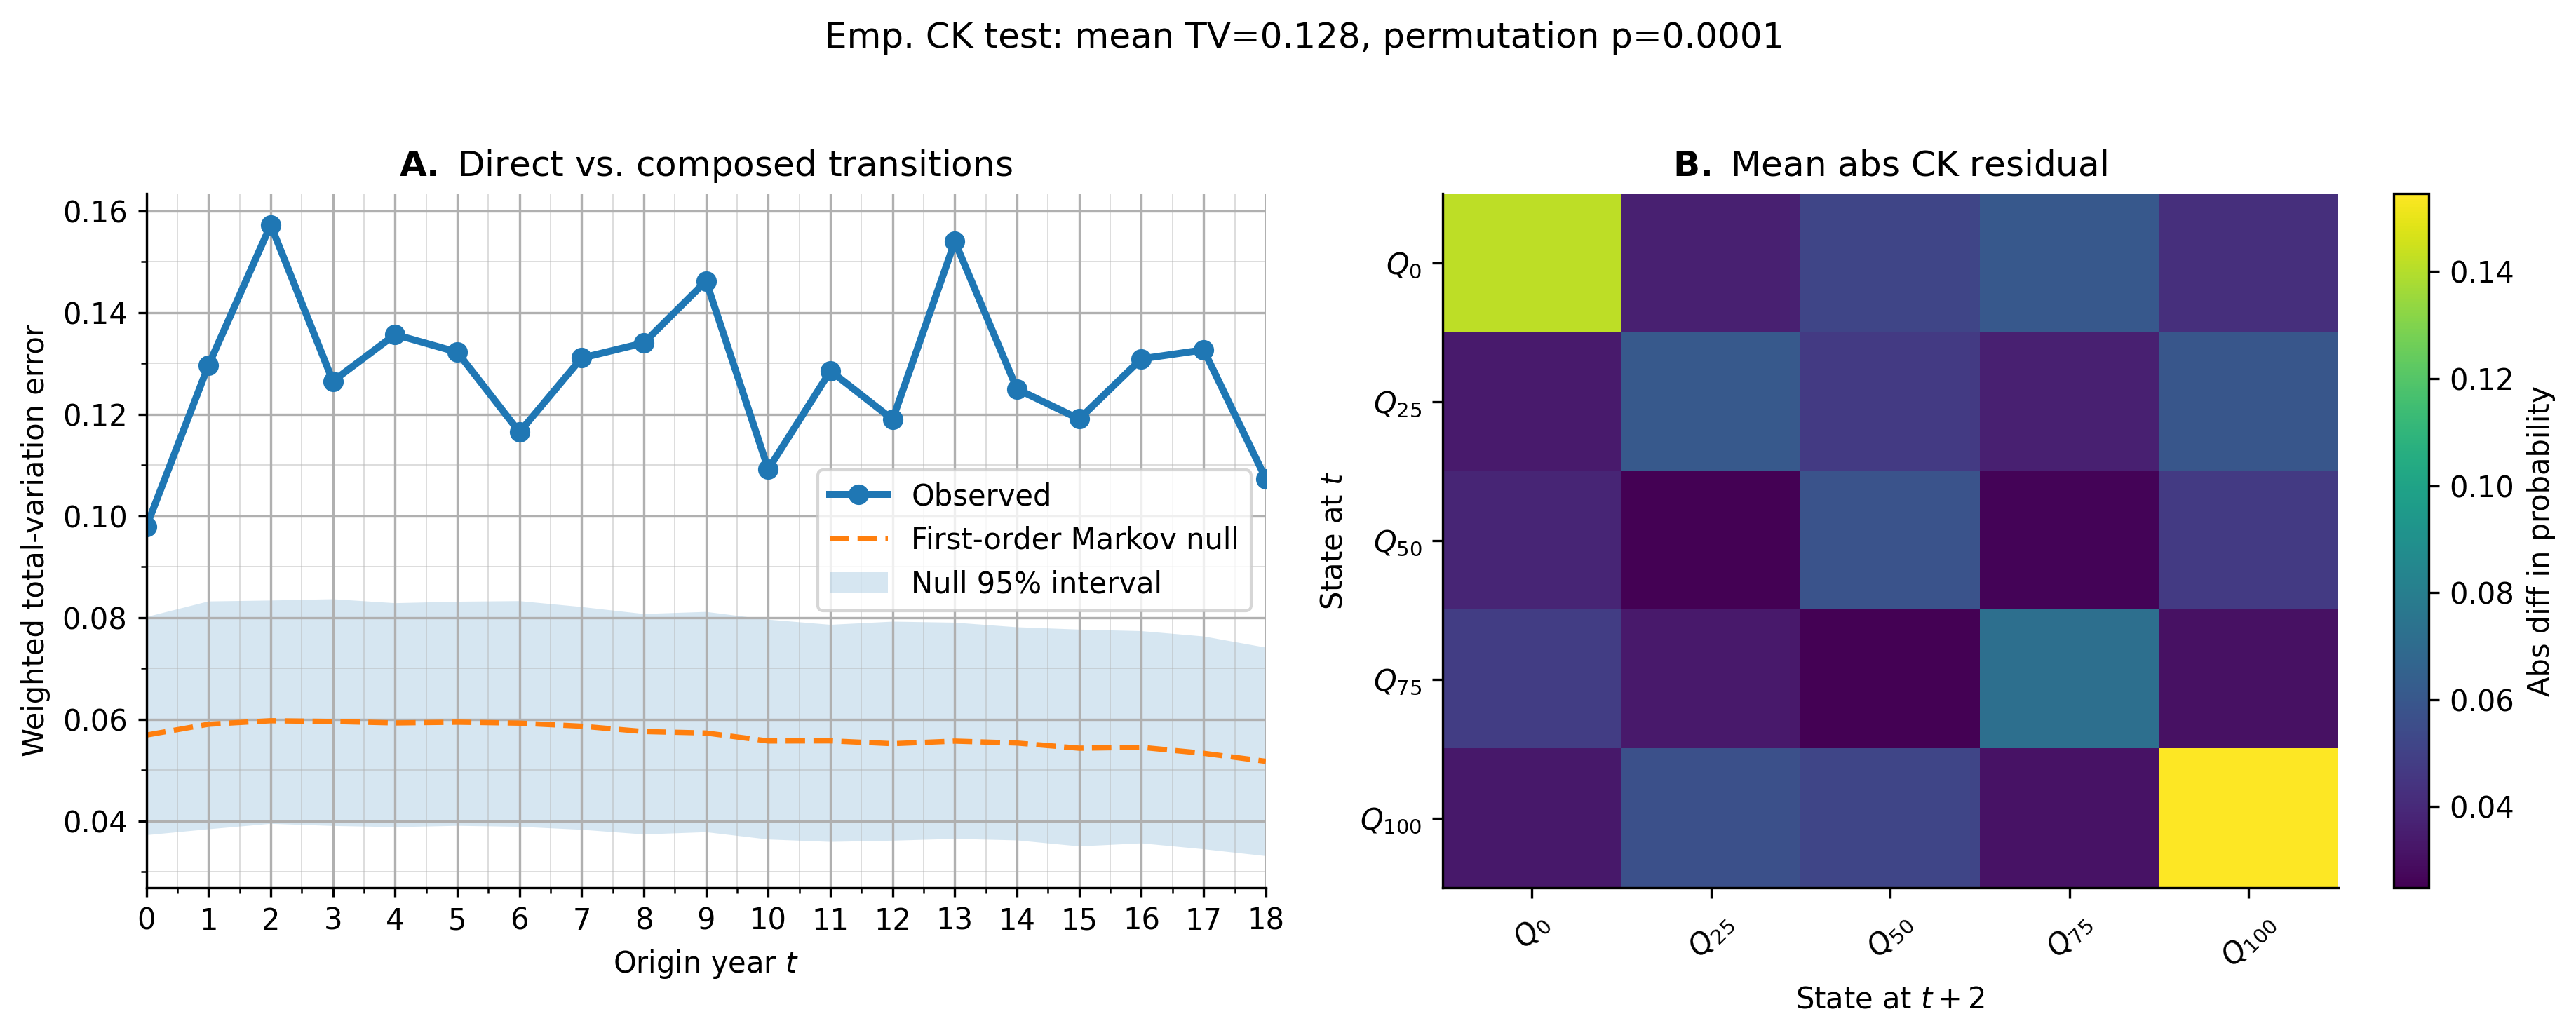
\includegraphics[width=0.87\linewidth]{figures/chapman_kolmogorov_test.png}
    \caption{Chapman-Kolmogorov results on $q_t$ as a first-order Markov state. \panel{a} The blue line shows error between observed transitions from $t$ to $t+2$ and those expected by composing intermediate transition matrices. The total variation error averages the probability mass that must be reconfigured to align the distributions. The shaded region shows expected error under the null. The observed error is above the 95\% CI in all origin years, indicating a persistent discrepancy. \panel{b} We split the data into an exact-zero state and four positive productivity quartile bins, $ Q_{25}, Q_{50}, Q_{75}, Q_{100}$. The heatmap depicts which of the transitions most contribute to the failure. The brightest cells are $Q_0\rightarrow Q_0$ and $Q_{100} \rightarrow Q_{100}$.}
    \label{fig:CK_test}
\end{figure*}

We experienced similar failure modes across a wide array of models diverse enough to share only one commonality: they were all generally first-order Markovian in $q_t$. We already knew there were some signatures of non-Markovian behavior in the productivity data. Given that, we turned back to more rigorously appraise the structure of the empirical data.

\subsection{Chapman-Kolmogorov test of \texorpdfstring{$q_t$}{q_t}}
\label{emp_motivation:ck_qt}
We performed a Chapman-Kolmogorov test on the data. If $q_t$ is the complete/sufficient state of a career in our first-order, age-dependent Markov process, observed two-year transitions should agree with the transitions obtained by chaining together one-year transitions. 

We found that the use of $q_t$ as a first-order Markov state is not supported by a first-order Chapman-Kolmogorov test, which rejects the required consistency. With 10,000 conditional permutations of the data, we obtained a conditional-permutation \textit{p}-value of $0.0000999$. Not one of the permuted datasets gave an error like the empirical one, so we rejected the null hypothesis. As shown in \Cref{fig:CK_test}B, a first-order $q_t$ especially misrepresents persistence at the extremes.

The CK test suggests that $q_t$ is an insufficient first-order Markov state under the test parameters, but does not by itself show that earlier history improves prediction. We therefore compared a current-state model against a history-aware model.

\subsection{Held-out history impact}
\label{emp_motivation:held_out_history}

Using three horizons $h \in \{1,2,5\}$, we tasked two models to predict log-productivity $z_{t+h} = \log (q_{t+h} + \epsilon)$ and rank $R_{t+h}$. One model is only aware of the current year, current productivity, and current activity state. The other model has access to $\mathbf{h}_t$, a history vector including: 
\begin{itemize}
    \item \texttt{dz1}, the most recent change in log productivity,
    \item \texttt{slope3}, the slope over the three most recent years,
    \item \texttt{sd3}, the most recent three-year volatility,
    \item \texttt{log\_cum\_q}, cumulative log-productivity through the current year,
    \item \texttt{drawdown}, the distance between the last maximum and current productivity,
    \item \texttt{active\_run}, the length of the current consecutive run of active years, 
    \item \texttt{zero\_run}, the length of the current consecutive run of zero years.
\end{itemize}
More schematically, model $X_{\text{base}} = (t,z_t, \mathbbm{1}\{q_t >0\})$ and $X_{\text{history}} = (t,z_t, \mathbbm{1}\{q_t >0\}, \mathbf{h}_t)$. This answers the question "Does history add predictive information after the current state is already known?"

We fit both models with scikit-learn's \texttt{HistGradientBoostingRegressor}, allowing for learning of nonlinear interactions. We used five-fold validation grouped by scholar and computed the results as $\operatorname{MAE}_{\text{gain}} = \operatorname{MAE}(X_{\text{base}}) - \operatorname{MAE}(X_{\text{history}})$.

\begin{figure*}[!t]
    \centering
    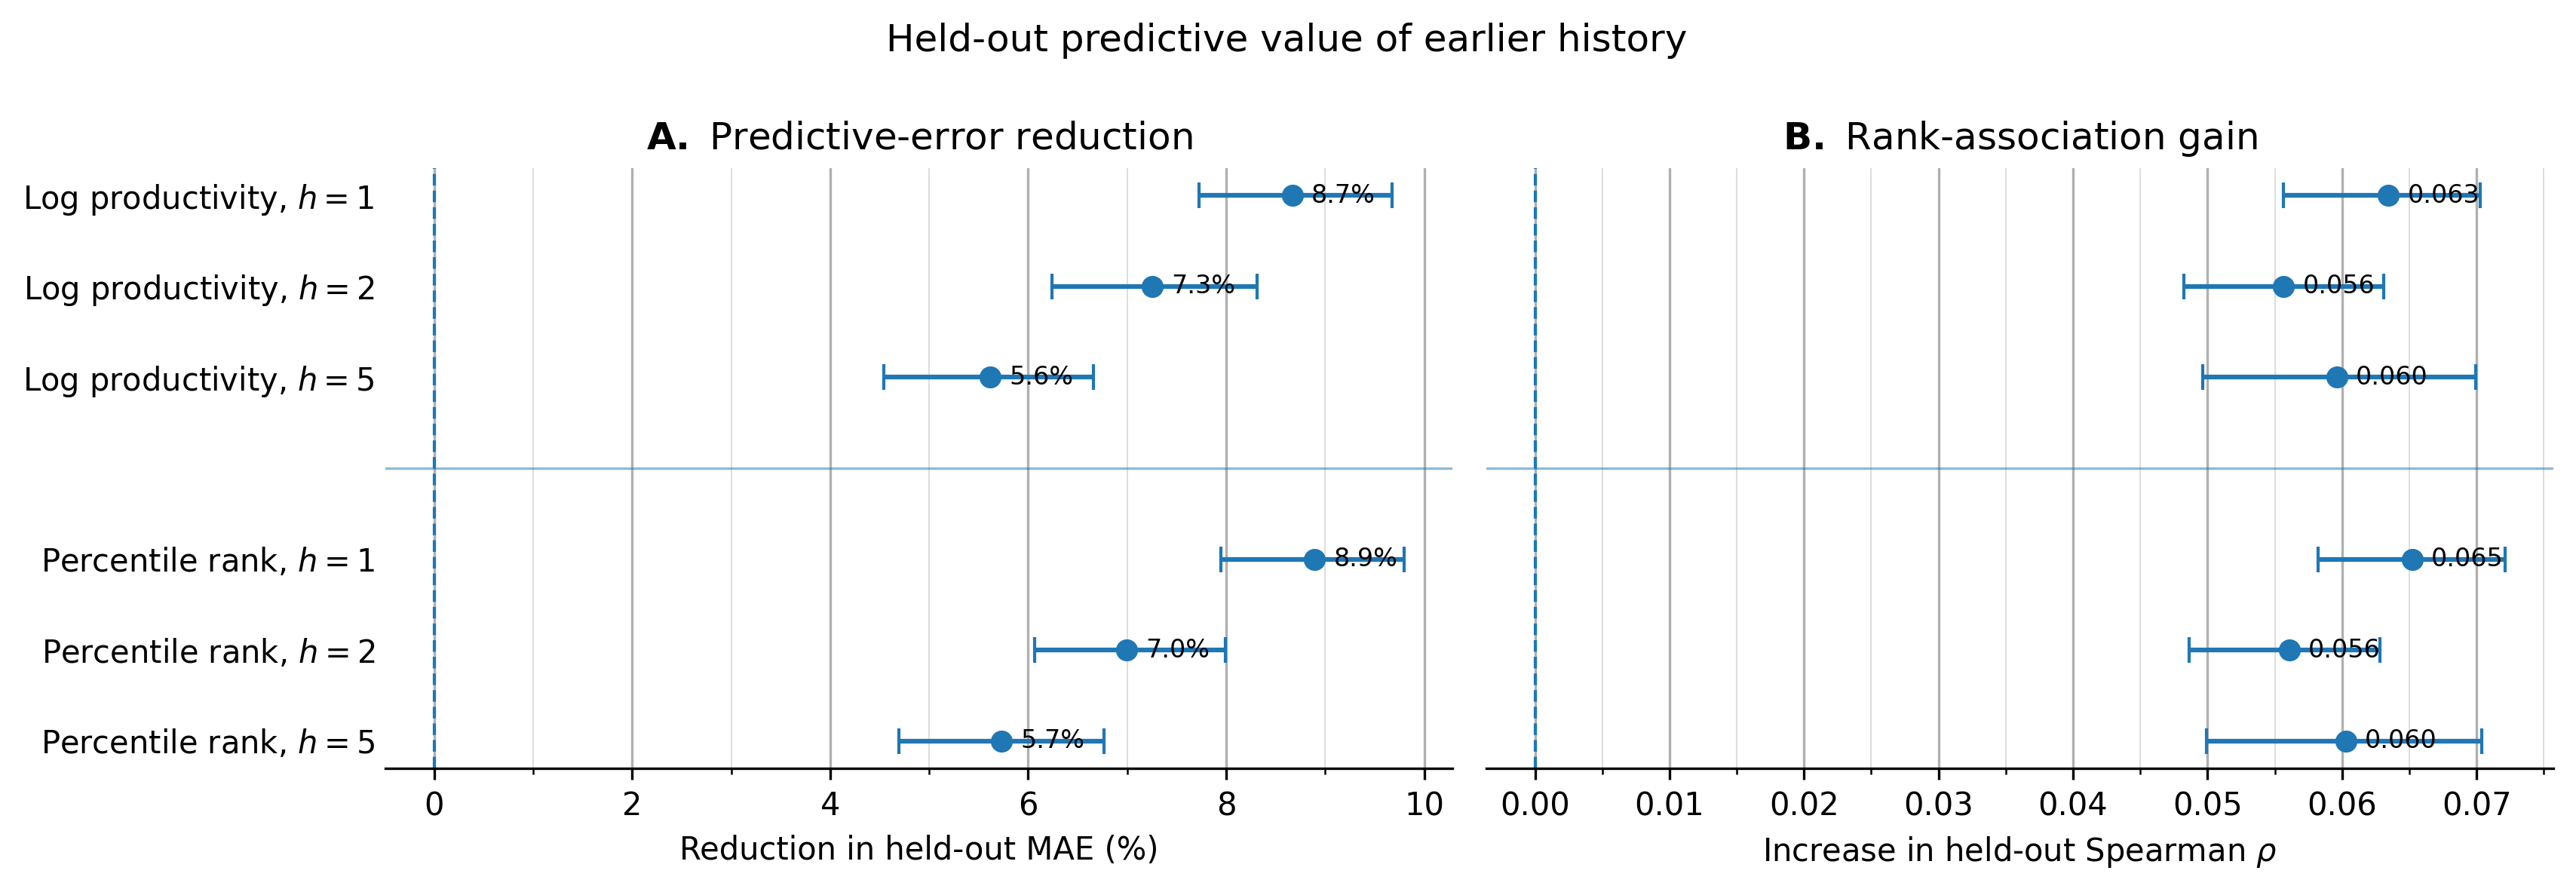
\includegraphics[width=0.87\linewidth]{figures/history_predictive_gain_forest.png}
    \caption{Forest plot of predictive gains. \panel{A} Reduction in error across the three horizons in both productivity and rank predictive ability. \panel{B} Gain in rank correlation in both tasks. Including earlier history  improves performance of a model. Of note, while MAE improvements decline monotonically with horizon distance, rank association does not.}
    \label{fig:history_predictive_gain_forest}
\end{figure*}

For all six tasks, we identified an improvement in MAE with $X_{\text{history}}$, and all six 95\% CIs exclude zero. Further, we computed all six comparative Spearman correlations $\rho(R_h, \hat{R}_h)$, finding that in each case, $X_{\text{history}}$ outperforms $X_{\text{base}}$, as shown in \Cref{fig:history_predictive_gain_forest}. This test supports the conclusion that, based on structures within the empirical data, history improves predicted magnitude and ordering, and thereby supports a class of history-aware models, although it does not justify our exact design. 

\subsection{Diminishing returns to autoregressive order}
\label{emp_motivation:ar_order}

We must resolve the justification of history-aware models with poor results from past autoregressive models. To do so, we tested a series of architecturally identical $\operatorname{AR}(p)$ models of increasingly higher $p$. 

\begin{figure}[H]
    \centering
    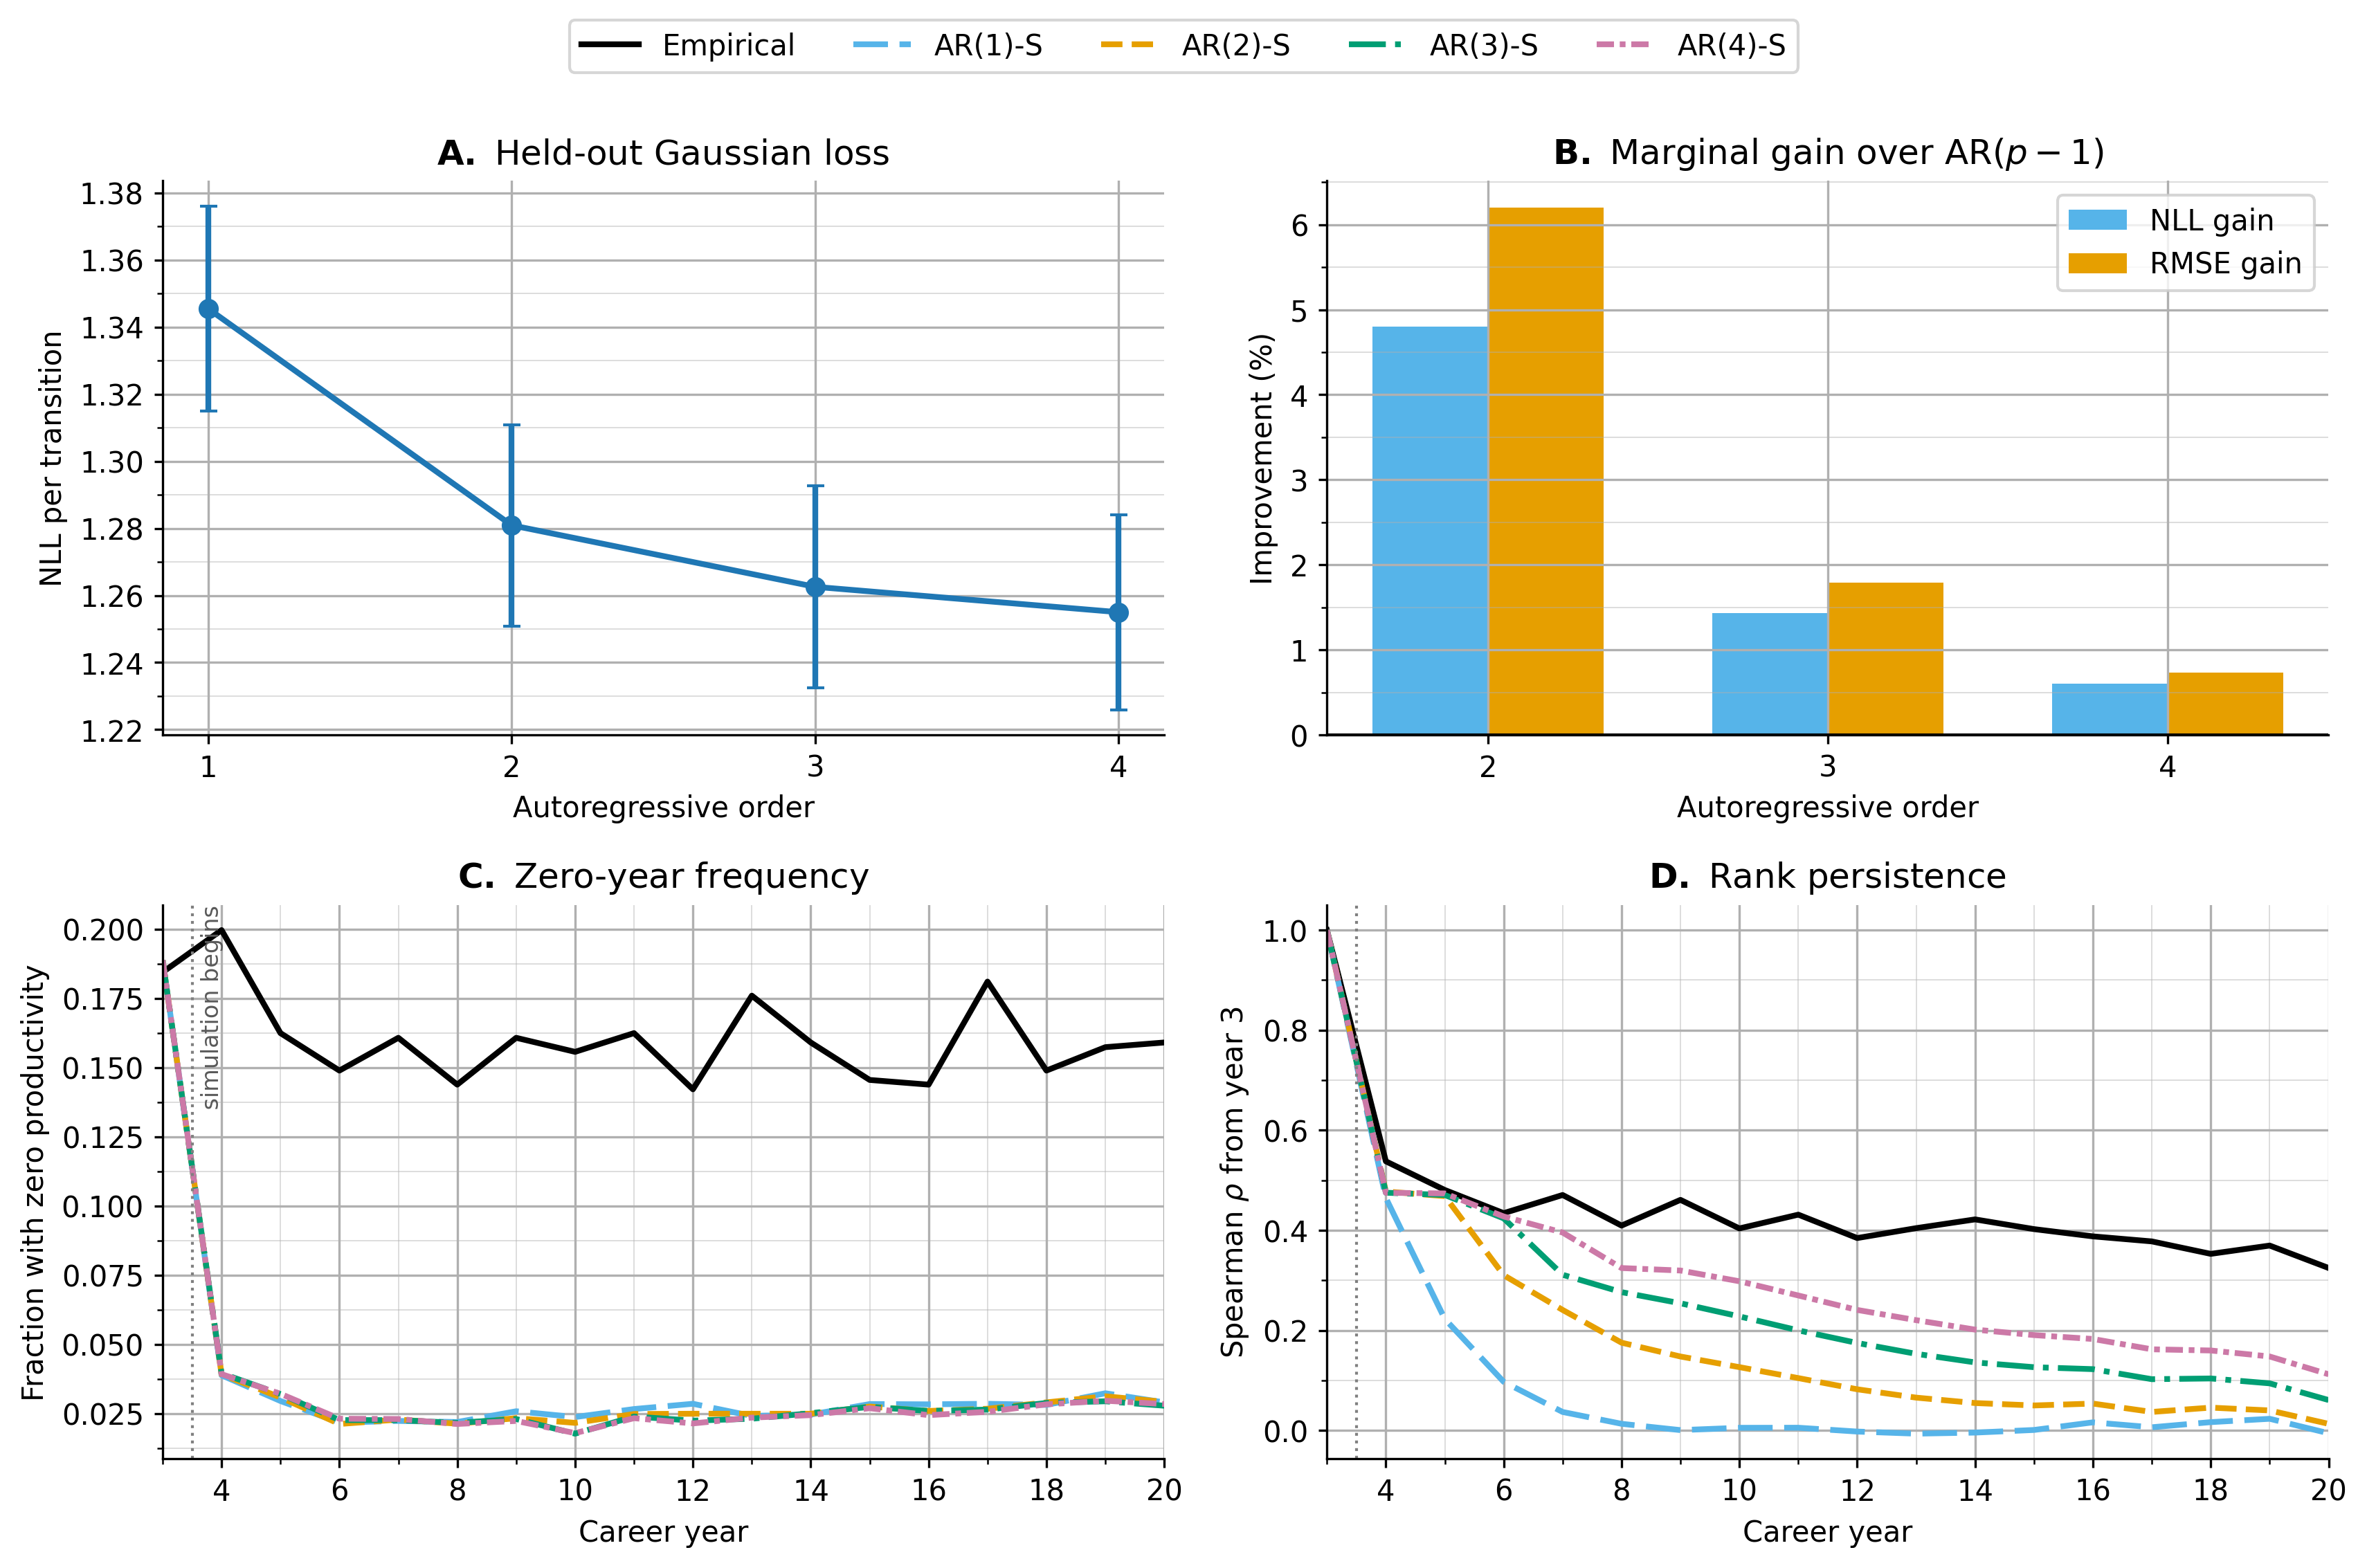
\includegraphics[width=1\linewidth]{figures_ar_p/ar_order_bridge.png}
    \caption{$\operatorname{AR}(p)$ diagnostics. \panel{A} The held-out NLL changes little beyond $\operatorname{AR}(2)$. \panel{b} Marginal gain of $\operatorname{AR}(p)$ over $\operatorname{AR}(p-1)$. Almost all improvement is gained at $\operatorname{AR}(2)$. \panel{c} no tested $\operatorname{AR}(p)$ solves inactivity. \panel{d} Increasing $p$ improves rank mixing, but still falls well short of empirical.}
    \label{fig:ar_order_bridge}
\end{figure}

We found sharply diminishing returns in model improvement with respect to increasing order. The main body of improvement is found between $\operatorname{AR}(1)$ and $\operatorname{AR}(2)$; beyond that, improvements are slight, and all $\operatorname{AR}(p)$ models tested share fundamental limitations imparted by their structure, not their order. These results, and the other results from this experiment in \Cref{supp:arp_diminishing}, clearly show that while history matters, attempting to factor it in with separate lags up to $p=4$ does not fix certain structural limitations.
 
Our last empirical test gave us a rigorous answer to our rank-mixing problems. We used a nonparametric kNN to try and model rank-mixing, and found that even that model collapsed to zero (see \Cref{supp:held_out_rank_mixing}), suggesting that the tested flexible $q_t$-only representation still omitted information needed for long-run persistence. 

Together, these tests indicate that current productivity alone is insufficient and that earlier history improves prediction. They also show that adding separate lags through $p=4$ does not resolve the tested generative failures. This motivated a compressed history state rather than a longer finite lag vector.

To appraise this new approach, we designed a simple, parsimonious self-exciting hurdle. In doing so, we continued with work recommended in \textit{Scientific Productivity as a Random Walk}.

\section{Design}
\label{sec:design}
Broadly speaking, this is a self-exciting autoregressive hurdle model. Its extensive margin is a simple logistic regression, its intensive margin is a simple log-linear regression, and its history term is an EWMA. Hawkes processes are a prominent class of self-exciting models; although inspired by them, this model is not one, as elaborated on in \Cref{supp:hawkes_v_se_h_s}. 

For ease of understanding, Greek coefficients moderate entry into a productive state and Latin coefficients moderate productivity. 

We first define $H_t$, the compressed history state from $0$ to $t-2$ (because $t-1$ is directly called in the intensive and extensive equations):
\begin{equation}
    H_t =\frac{\sum_{\tau=0}^{t-2}\rho^{\,t-2-\tau}\log(1+q_{\tau})}{\sum_{\tau=0}^{t-2}\rho^{t-2-\tau}}
\label{eq:history_state}
\end{equation}
In words, that is the exponentially weighted mean of log1p past productivity, normalized by the exponential weights. More recent years receive exponentially greater weight. The global parameter $\rho$ is fitted once and controls the rate of decay. The fitted value for $\rho$ was 0.6664, or a memory half-life of $\approx 1.71$ years.

Having defined history, we compute the extensive margin, or the log-odds of being active at $t$. Let $w = \mathbbm{1}\{(q_{t-1} >0)\}$, an indicator function for the productivity state of the previous year. Then:
\begin{equation}
    \operatorname{logit}\text{Pr}(q_t > 0) = \alpha_s +\beta_s\log(1+q_{t-1}) +\gamma_sw+\delta_s H_{t},
\label{eq:extensive_margin}
\end{equation}
Conditioned on $q_t >0$, we compute the log-productivity for the current year as:
\begin{equation}
    \log q_t = a_s +b_s\log(1+q_{t-1}) +c_sw +d_sH_{t}+\epsilon_{t}
\label{eq:intensive_margin}
\end{equation}
where $\epsilon_t \sim \mathcal{N}(0, \sigma^2_s)$.

The parameters are arranged simply:
\begin{itemize}
    \item $\alpha$, \textit{a}: intercepts/baselines,
    \item $\beta$, \textit{b}: persistence of log1p of last year's productivity,
    \item $\gamma$, \textit{c}: weight of being active last year,
    \item $\delta$, \textit{d}: persistence of compressed history from $0$ to $t-2$,
    \item $\sigma^2$: the variance of the shock distribution.
\end{itemize}

Exponential weighting provides a recursively updating finite state governed by one global decay parameter $\rho$. It permits earlier productivity to remain informative without the permanent accumulation characteristic of a geometric random walk.

The design of this model draws on a significant body of literature in applied probability and statistics, reviewed in \Cref{supp:support_of_se}, but we are not aware of any previous application of this particular architecture to our line of inquiry.

\section{Results}
\label{sec:results}
We compare the results of SE-Hurdle-S against a selection of past models against which we could benchmark the model (see \Cref{supp:past_models} for refreshers on the design of old models).

\subsection{Laplace-like raw increments}
\label{results:laplace_distribution}
In \Cref{fig:raw_increment_laplace_pooled}, we plotted the pooled distributions of raw increments and their Laplace fit characteristics. SE-Hurdle-S reproduced a Laplace-like distribution of raw increments, with some reservations.
%%% FIGURE PLACED HERE FOR ORDERING %%%
\begin{figure*}[!b]
    \centering
    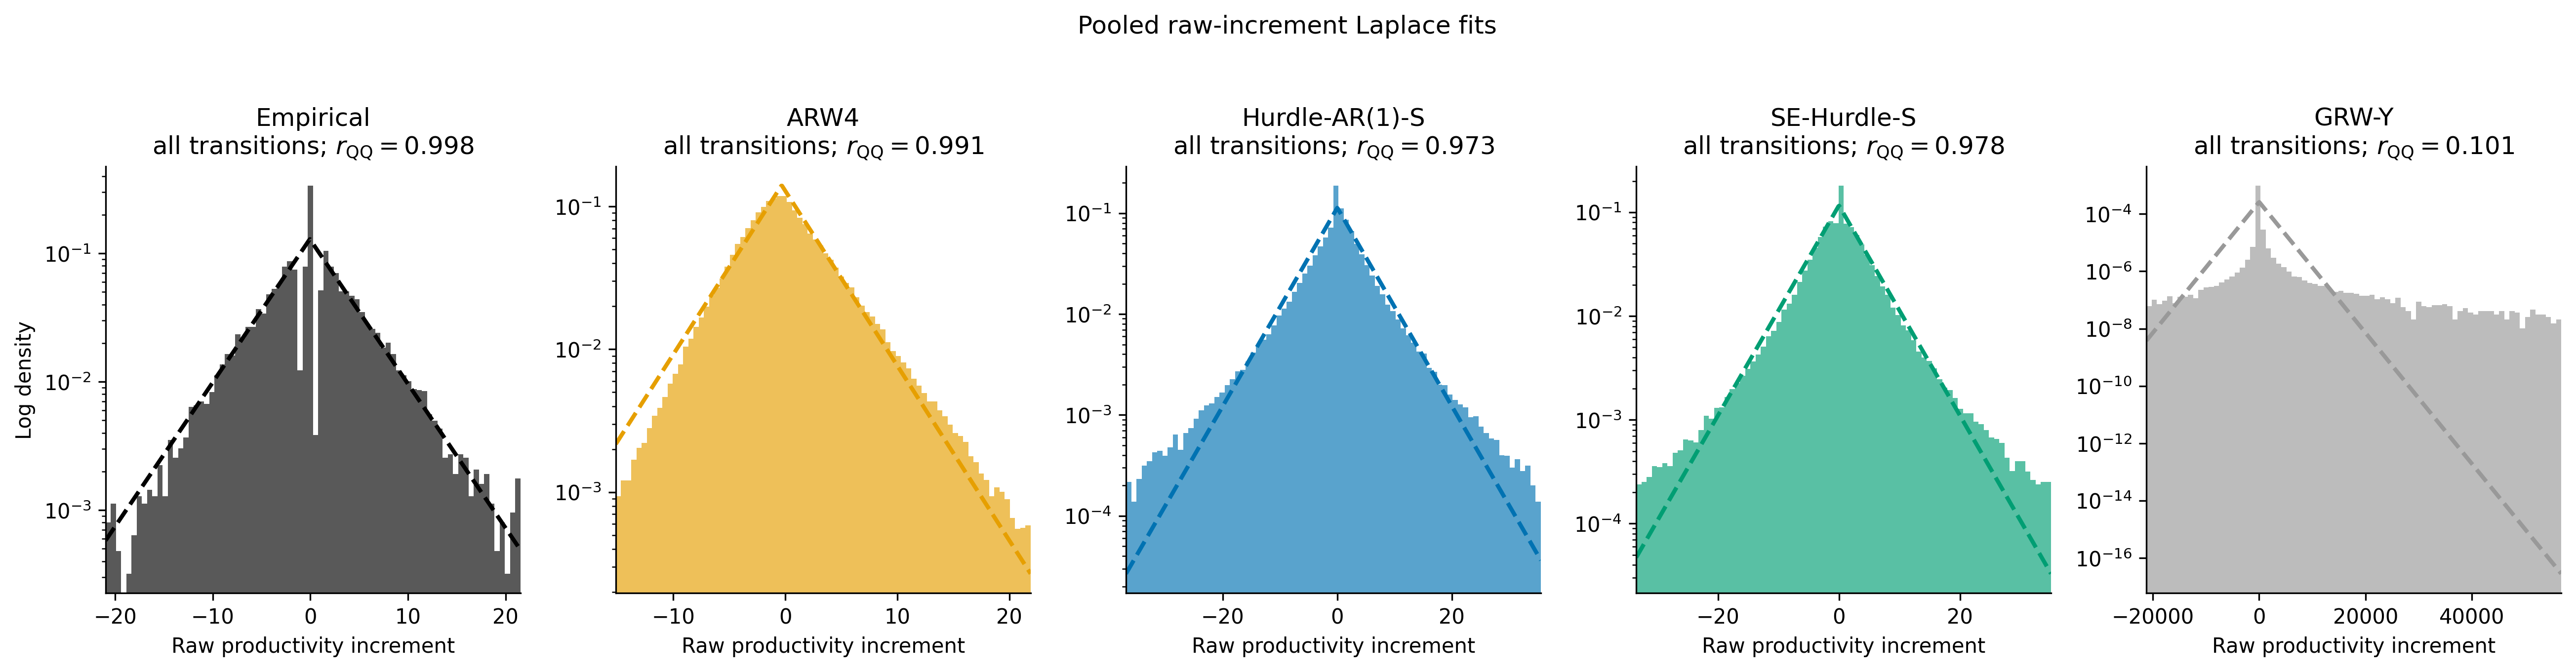
\includegraphics[width=1\linewidth]{figures/raw_increment_laplace_pooled.png}
    \caption{Fitted Laplace distributions of raw increments across various models. Our new model outperforms Hurdle-AR(1)-S and its Laplace $r_{\text{QQ}}$ scores are very near empirical. However, the overall visual fit is still somewhat off, with slightly heavier tails and narrower center than empirical data, suggestive of lingering inaccurate variance.}
    \label{fig:raw_increment_laplace_pooled}
\end{figure*}
%%% FIGURE PLACED HERE FOR ORDERING %%%
As has been well-documented, ARW4 displays a visually consistent but overall right-biased distribution, a property structurally inherent to that model (see \Cref{supp:arw4}). GRW-Y displays the enormous x-axis and comet shape associated with its failure mode. 

Going by $r_{\text{QQ}}$ alone we saw SE-Hurdle-S outperform its precedents and closely match empirical, but visual inspection shows a complication. While annual productivity fluctuations have been found to be leptokurtic and characterizable by a Laplace distribution \cite{leptokurt}, the simulated distributions of AR(1)-S (not shown in \Cref{fig:raw_increment_laplace_pooled}) and Hurdle-AR(1)-S (and their yearwise cousins, also not shown) have been more leptokurtic, displaying a characteristic tent shape with fat tails and a narrow center. SE-Hurdle-S has the same issue; this may be an artifact of zero increments; it may also be that an exponential-power distribution describes both better. A brief investigation uncovers potential structures: more in \Cref{supp:exponential_power_increments}. For stagewise Laplace distributions and a deeper discussion of them, refer to \Cref{fig:raw_increment_laplace_stagewise}.

Crucially, SE-Hurdle-S contains no Laplace innovations. Its broad
tent-shaped increment distribution is therefore emergent from the
model architecture. However, the simulated distribution remains more
sharply peaked and heavier-tailed than the empirical nonzero
distribution, so we describe it as Laplace-like rather than exactly
Laplace.

\subsection{Rank-persistence}
\label{results:rank_persistence}

For the first time in this project, the simulated rank-persistence trajectory and confidence interval largely encompass the empirical trend. 

\begin{figure}[H]
    \centering
    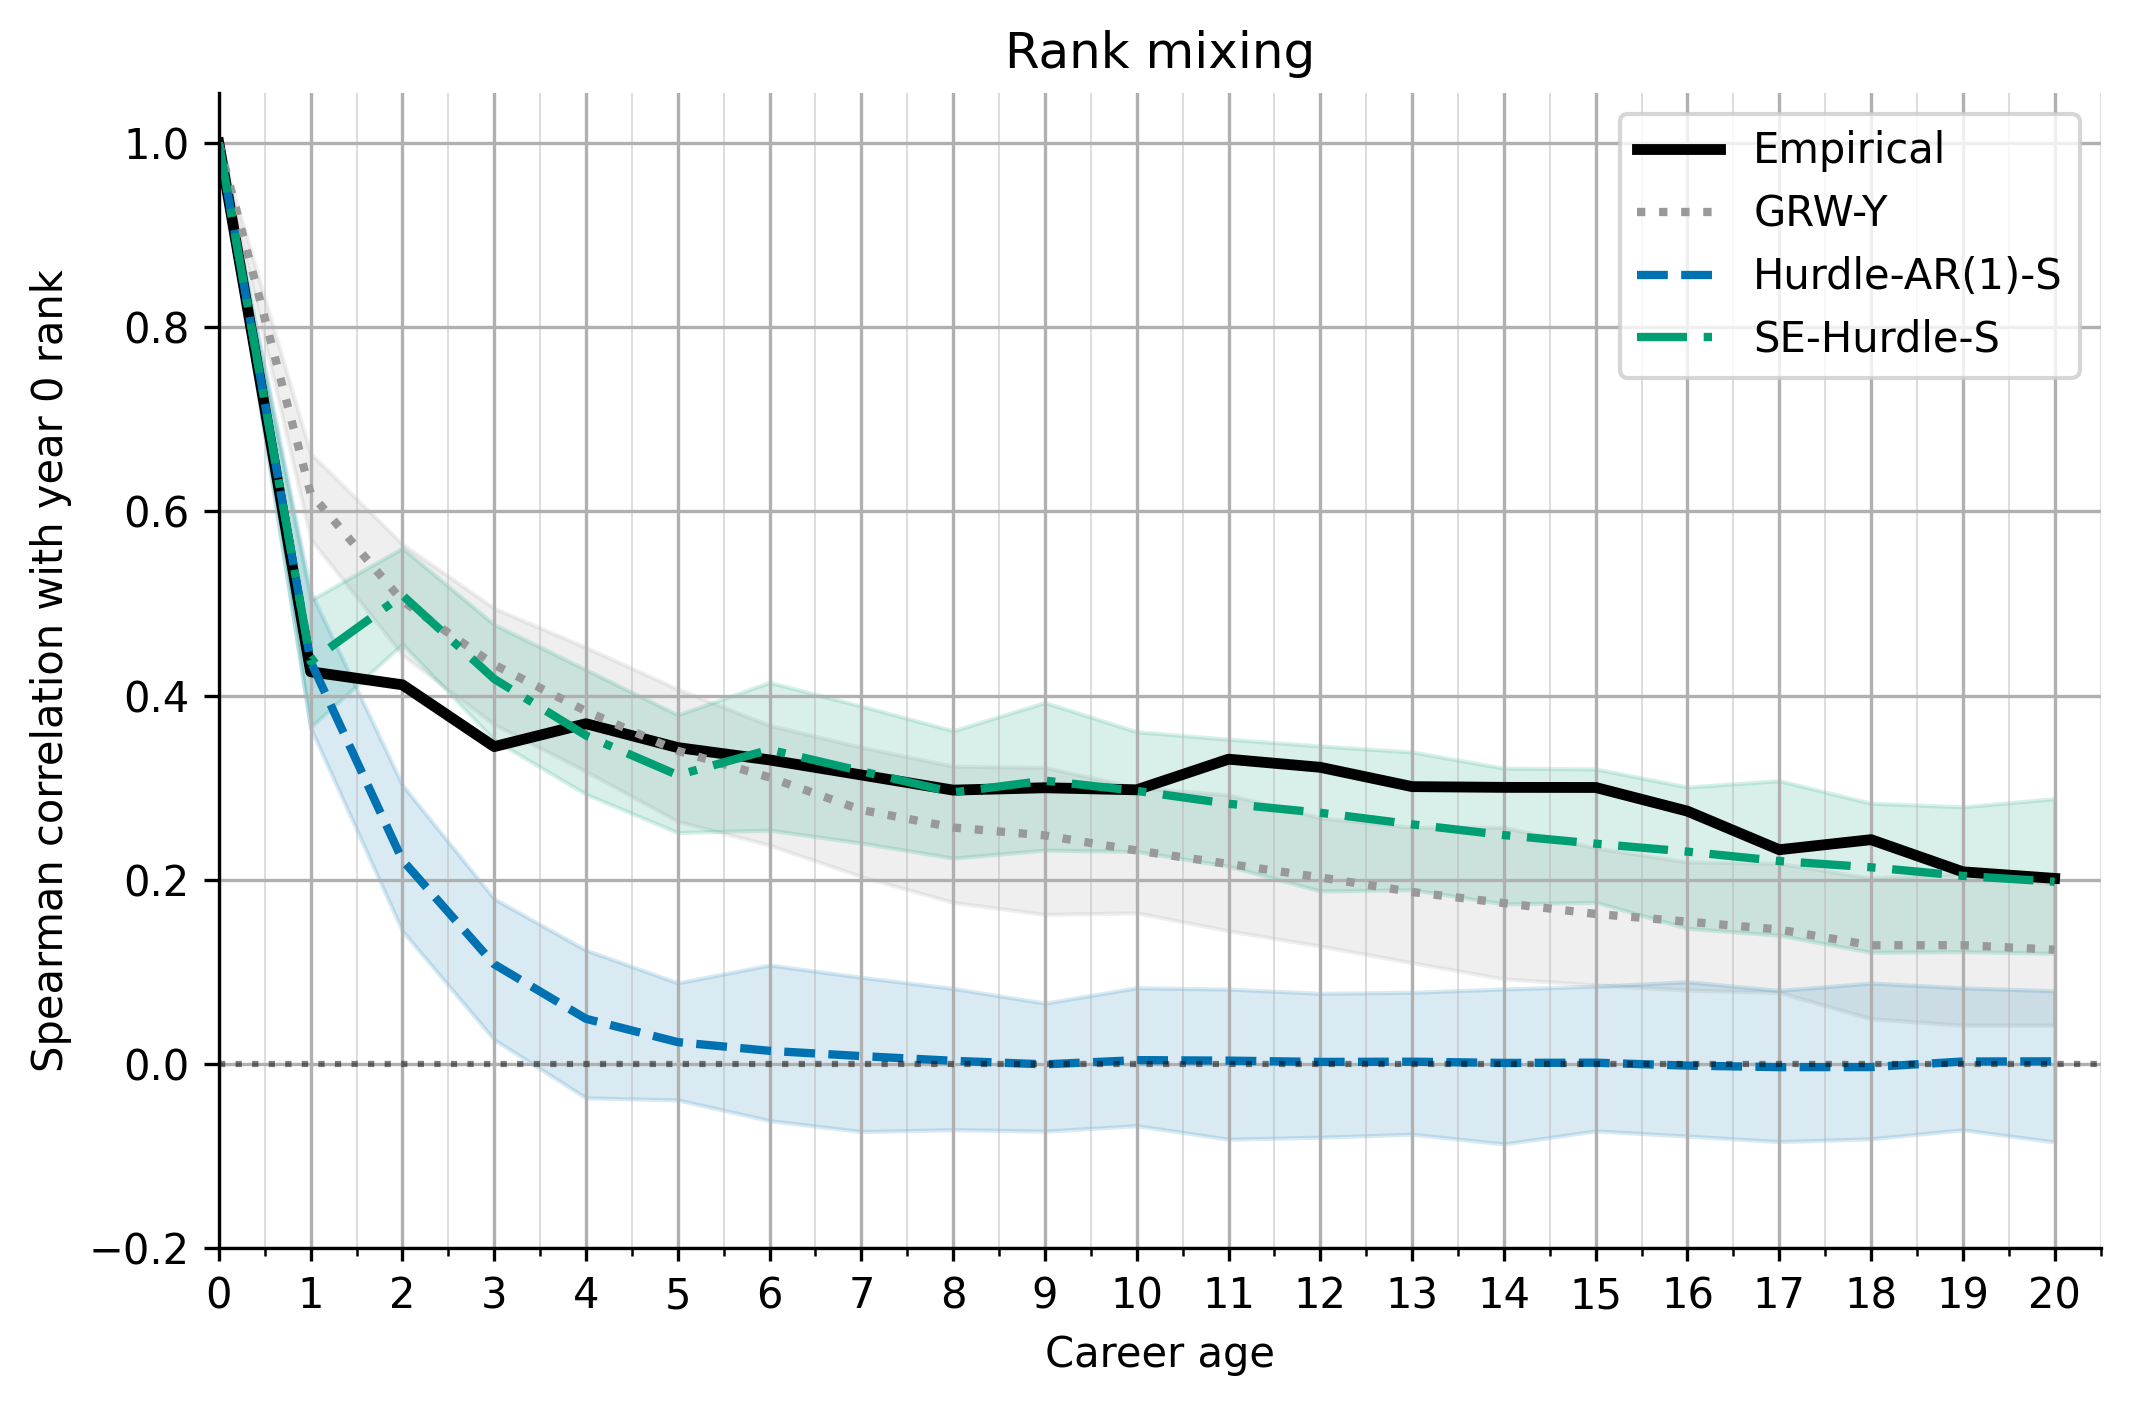
\includegraphics[width=1\linewidth]{figures/rank_mixing.png}
    \caption{Trend of $\rho(R_0,R_t)$ over time from several simulations against the empirical trajectory, with 95\% CIs.}
    \label{fig:rank_mixing}
\end{figure}

In contrast, Hurdle-AR(1)-S and its 95\% CI diverge from the empirical trend at $t=1$ and collapses to $\rho(R_0, R_t) = 0$ by $t = 8$; all other models we tested, except higher-order $\operatorname{AR}(p)$s (discussed in \Cref{supp:arp_diminishing}), did the same thing. The trend from GRW-Y displays the characteristic Spearman-correlation curve, a property explained in \Cref{supp:grw_rankmixing}.

\subsection{Trajectories of moments}
\label{results:trajectories_of_moments}

We compare the empirical trajectories of raw and log mean, median, and variance against SE-Hurdle-S, Hurdle-AR(1)-S, ARW4, and AR(1)-S.

\begin{figure}[H]
    \centering
    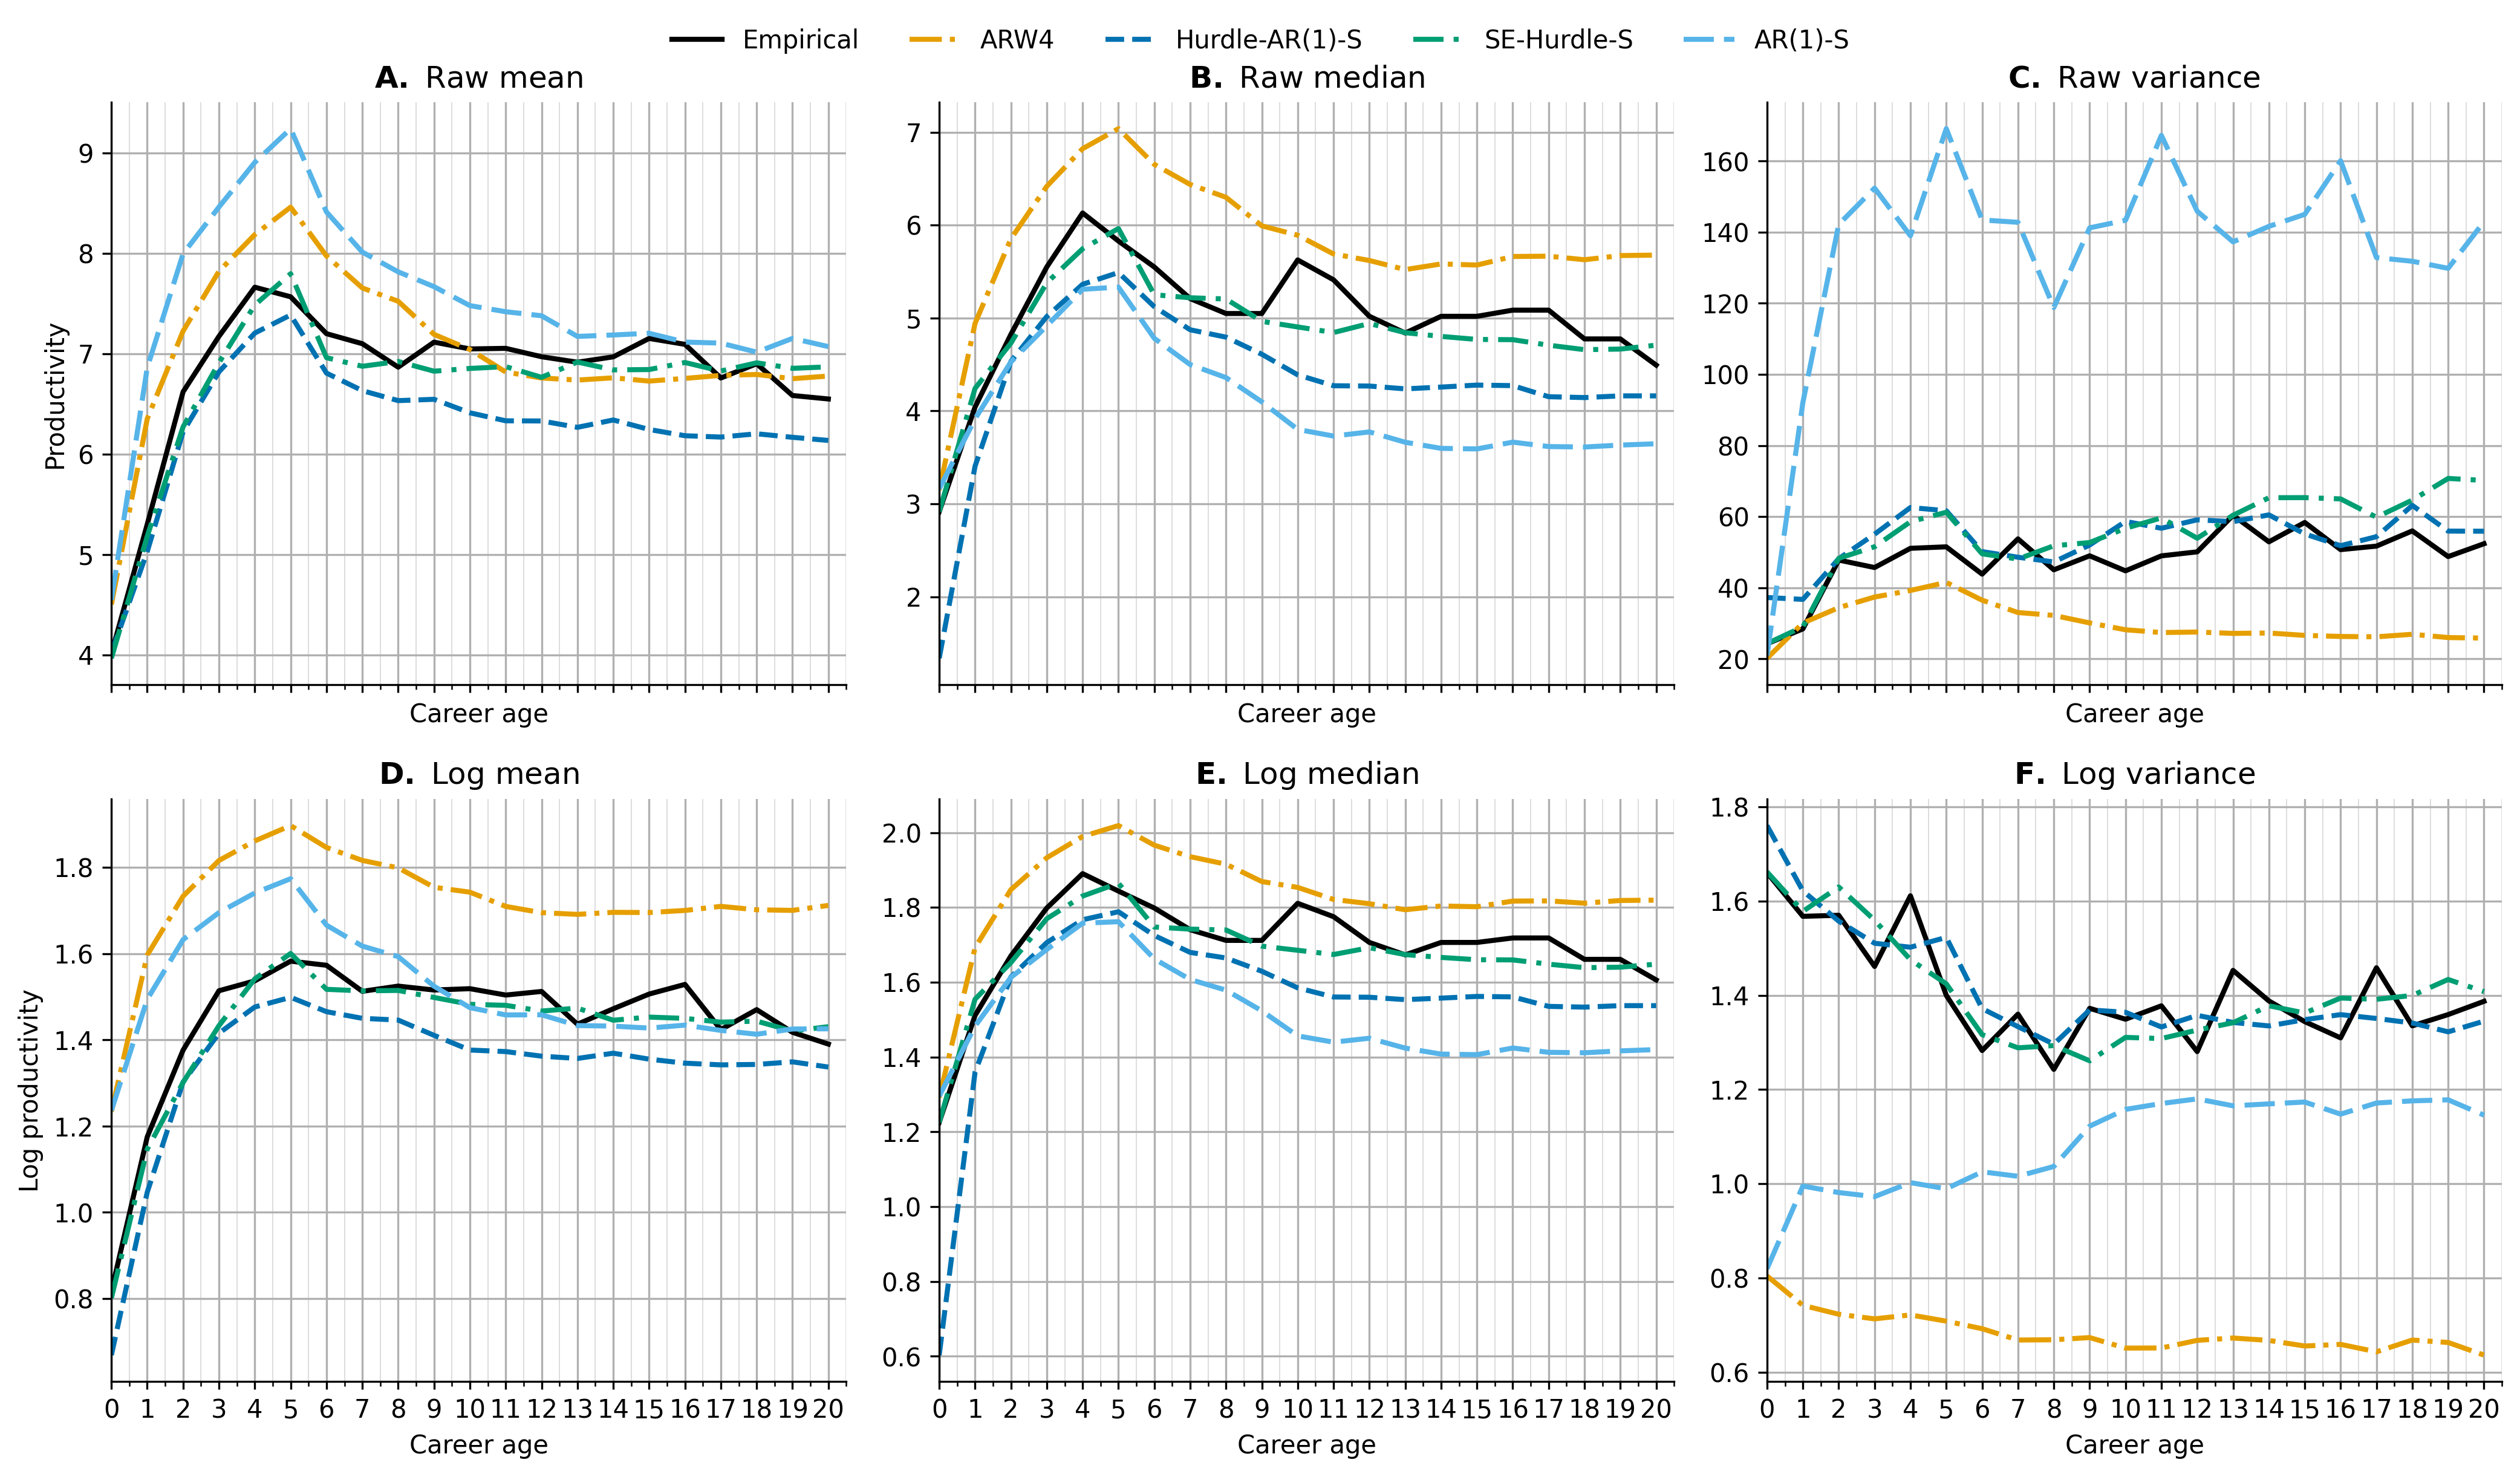
\includegraphics[width=1\linewidth]{figures/moment_trajectories.png}
    \caption{Moment trajectories in real and log space of assorted models against empirical data. See \Cref{supp:addl_figs_traj_moments} for higher-resolution subplots.}
    \label{fig:moment_trajectories}
\end{figure}

No model reproduces all six trajectories equally well, but their distinct failure modes are informative. SE-Hurdle-S most consistently reproduces the empirical center, Hurdle-AR(1)-S performs comparatively well on variance while remaining centered too low, ARW4 is underdispersed, and AR(1)-S is severely overdispersed in raw space.

All four models reproduce the broad rise and gradual decline of mean productivity. They also share a small temporal displacement: the empirical raw mean and median reach their early-career maxima at approximately $t=4$, while the simulated trajectories generally peak at approximately $t=5$. Beyond that shared displacement, SE-Hurdle-S follows the empirical mean and median most closely in both raw and log space. Hurdle-AR(1)-S instead settles below the empirical trajectories after the first several years, indicating that its productivity distribution is centered too low.

ARW4 and AR(1)-S both return superficially plausible mean trajectories, but their medians and variances show that they arrive there through opposing errors. ARW4 maintains an elevated median while underestimating variance, compressing careers into a too-narrow band of moderate productivity. AR(1)-S substantially underestimates the median while maintaining a more plausible mean, indicating that a small number of extreme trajectories raise the ensemble average. The mean alone therefore conceals underdispersion in ARW4 and severe right-tail overdispersion in AR(1)-S.

Variance remains the principal weakness of SE-Hurdle-S. Hurdle-AR(1)-S returns the closest raw variance trajectory, but this success must be considered alongside its underestimated mean and median: it reproduces approximately the correct amount of dispersion around the wrong center. ARW4 underestimates variance in both spaces, confirming that it suppresses too much empirical heterogeneity. AR(1)-S displays the opposite and most severe failure, producing raw variance far above the empirical trajectory.

SE-Hurdle-S lies between these extremes. Its log variance remains relatively close to empirical, but its raw variance becomes increasingly overestimated later in the career. This contrast is consistent with exponentiation amplifying modest excess dispersion in log productivity into a more consequential raw-space upper tail. Thus, SE-Hurdle-S avoids both the compressed distribution of ARW4 and the explosive behavior of AR(1)-S, but still allocates somewhat too much probability to highly productive outcomes.

Additional marginal checks show that SE-Hurdle-S also improves the distribution of within-career variation, although its pooled positive-year marginal remains similar to that of Hurdle-AR(1)-S (\Cref{supp:more_marginals}).

\subsection{Cumulative lognormality}
\label{results:cumulative_lognormality}
We assessed the normal QQ correlation of log-productivity of several models against empirical data. Between theoretical quantiles -1 and 1, the entire ensemble closely resembles the empirical shape and normal reference. Further, almost all of them capture the way the empirical data begins to fall short of the normal reference beyond theoretical quantile 1.5, with the exception of AR(1)-S, which remains closer to the normal reference than the rest of the ensemble.
\begin{figure}[H]
    \centering
    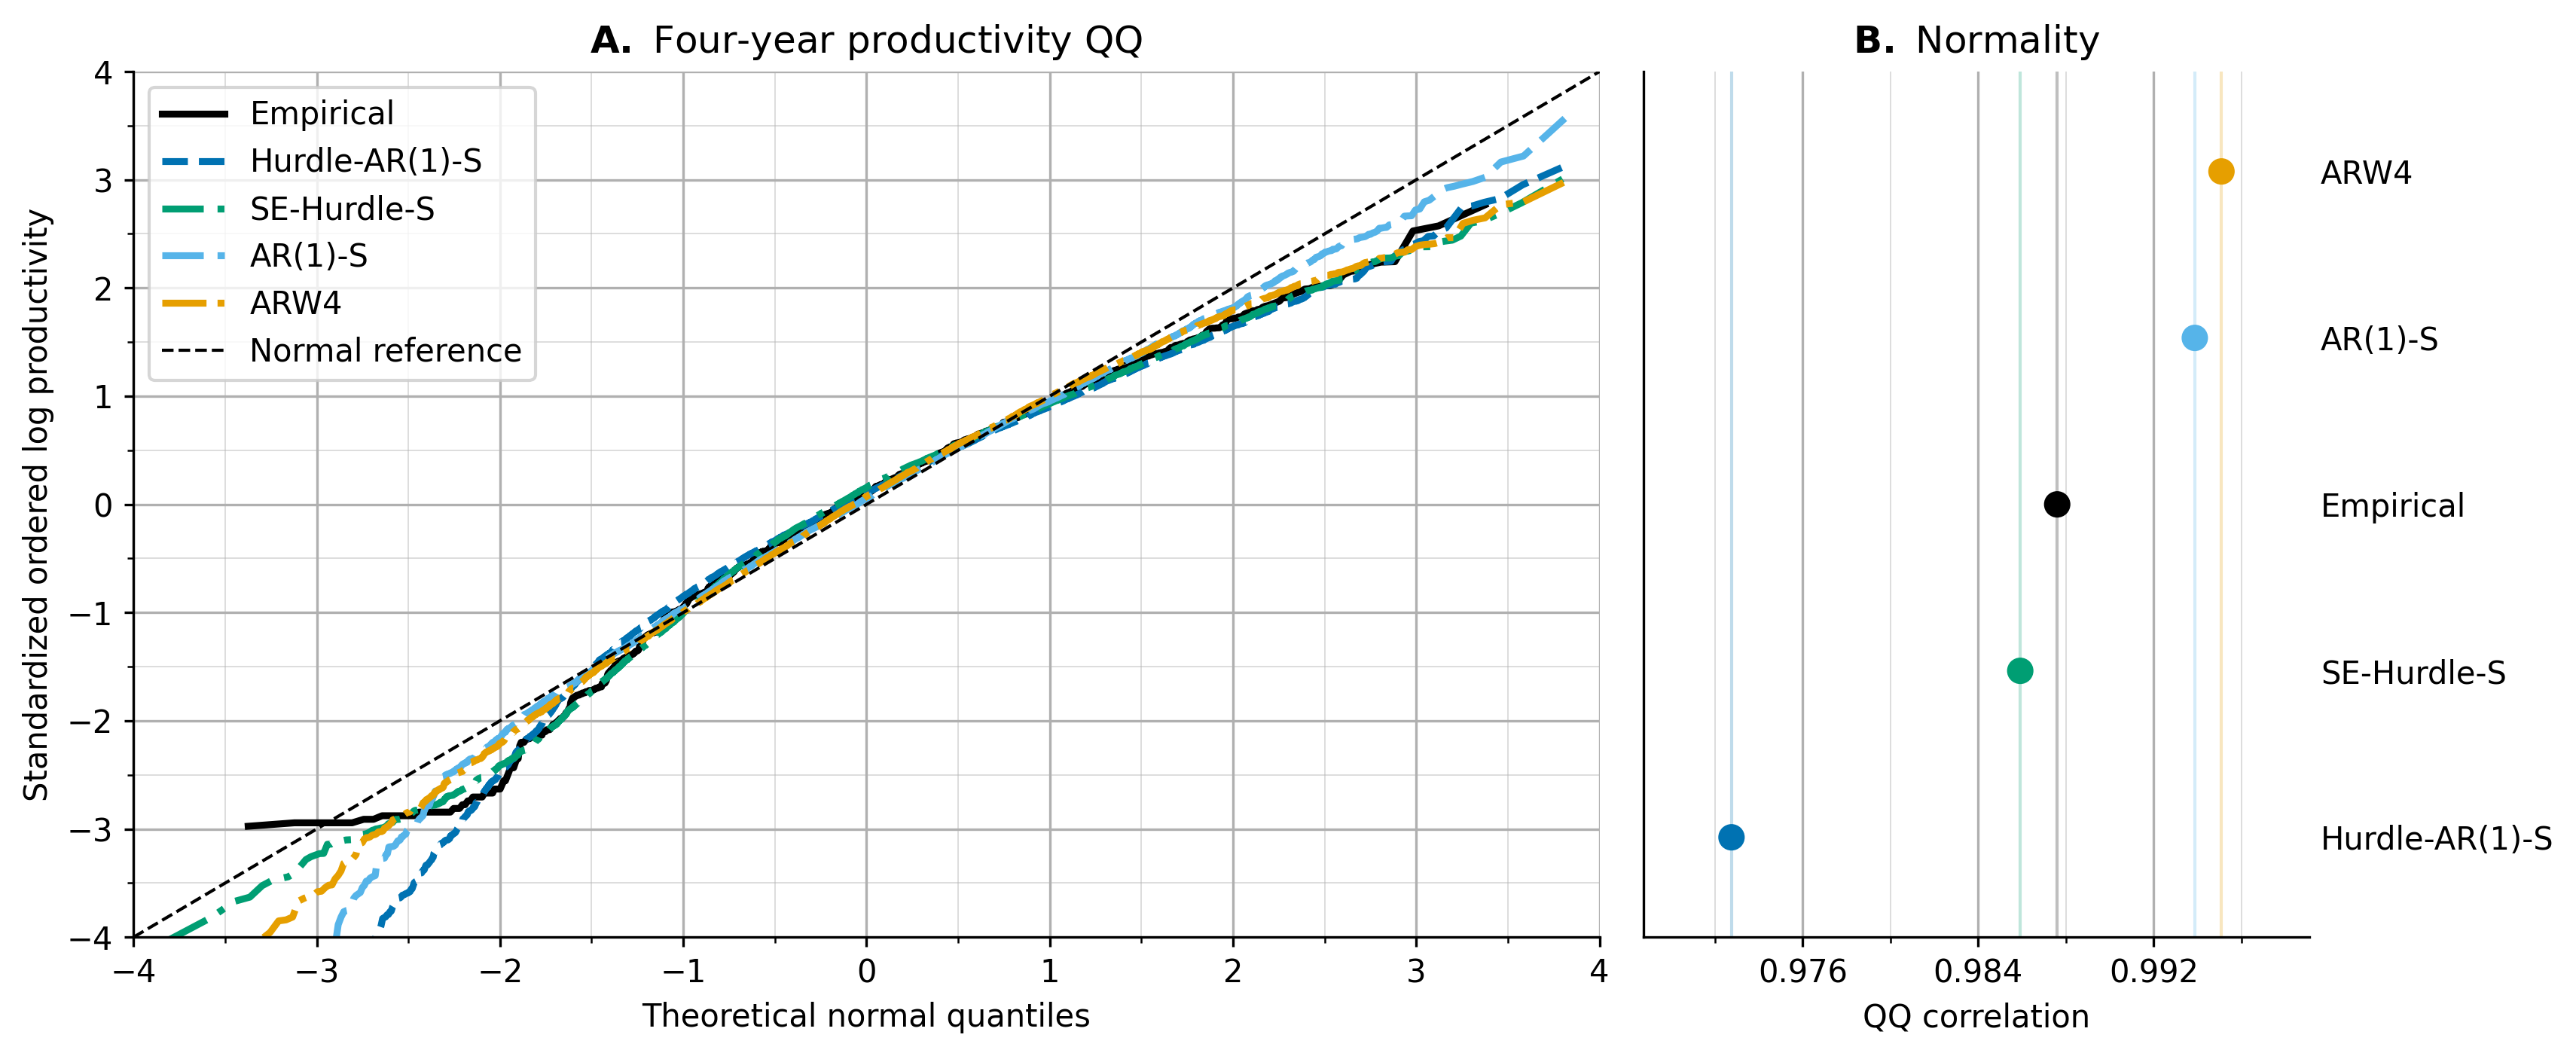
\includegraphics[width=1\linewidth]{figures/qq_last_four.png}
    \caption{QQ plots of cumulative last-four productivity. }
    \label{fig:qq_last_four}
\end{figure}
What is distinctive is what happens in the left tail. One persistent observation we encountered while using cumulative QQ plots was the fact that the empirical fit appears to have a lower bound at $-3$, a bottom that simulations fail to capture. As it turns out, this is an artifact of how we prepared the empirical data and defined our cumulative range. The exact analytical reason for the emergence of this phenomenon is discussed in \Cref{supp:lastfour_qq_left_tail}. 

In Panel \panel{b}, SE-Hurdle-S also performs most consistently with empirical data under our metrics; its QQ correlation is only slightly below empirical, while the other models variously score too high or low. This further supports the conclusion that SE-Hurdle-S is most consistent with empirical lognormality and signature tailed departures from lognormality.

In \Cref{supp:more_lognormal}, we discuss further results for SE-Hurdle-S with regard to its ability to closely match the distinctive shape of empirical 'lognormality'.

%%% FIGURE PLACED HERE FOR ORDERING %%%
\begin{figure*}[!t]
    \centering
    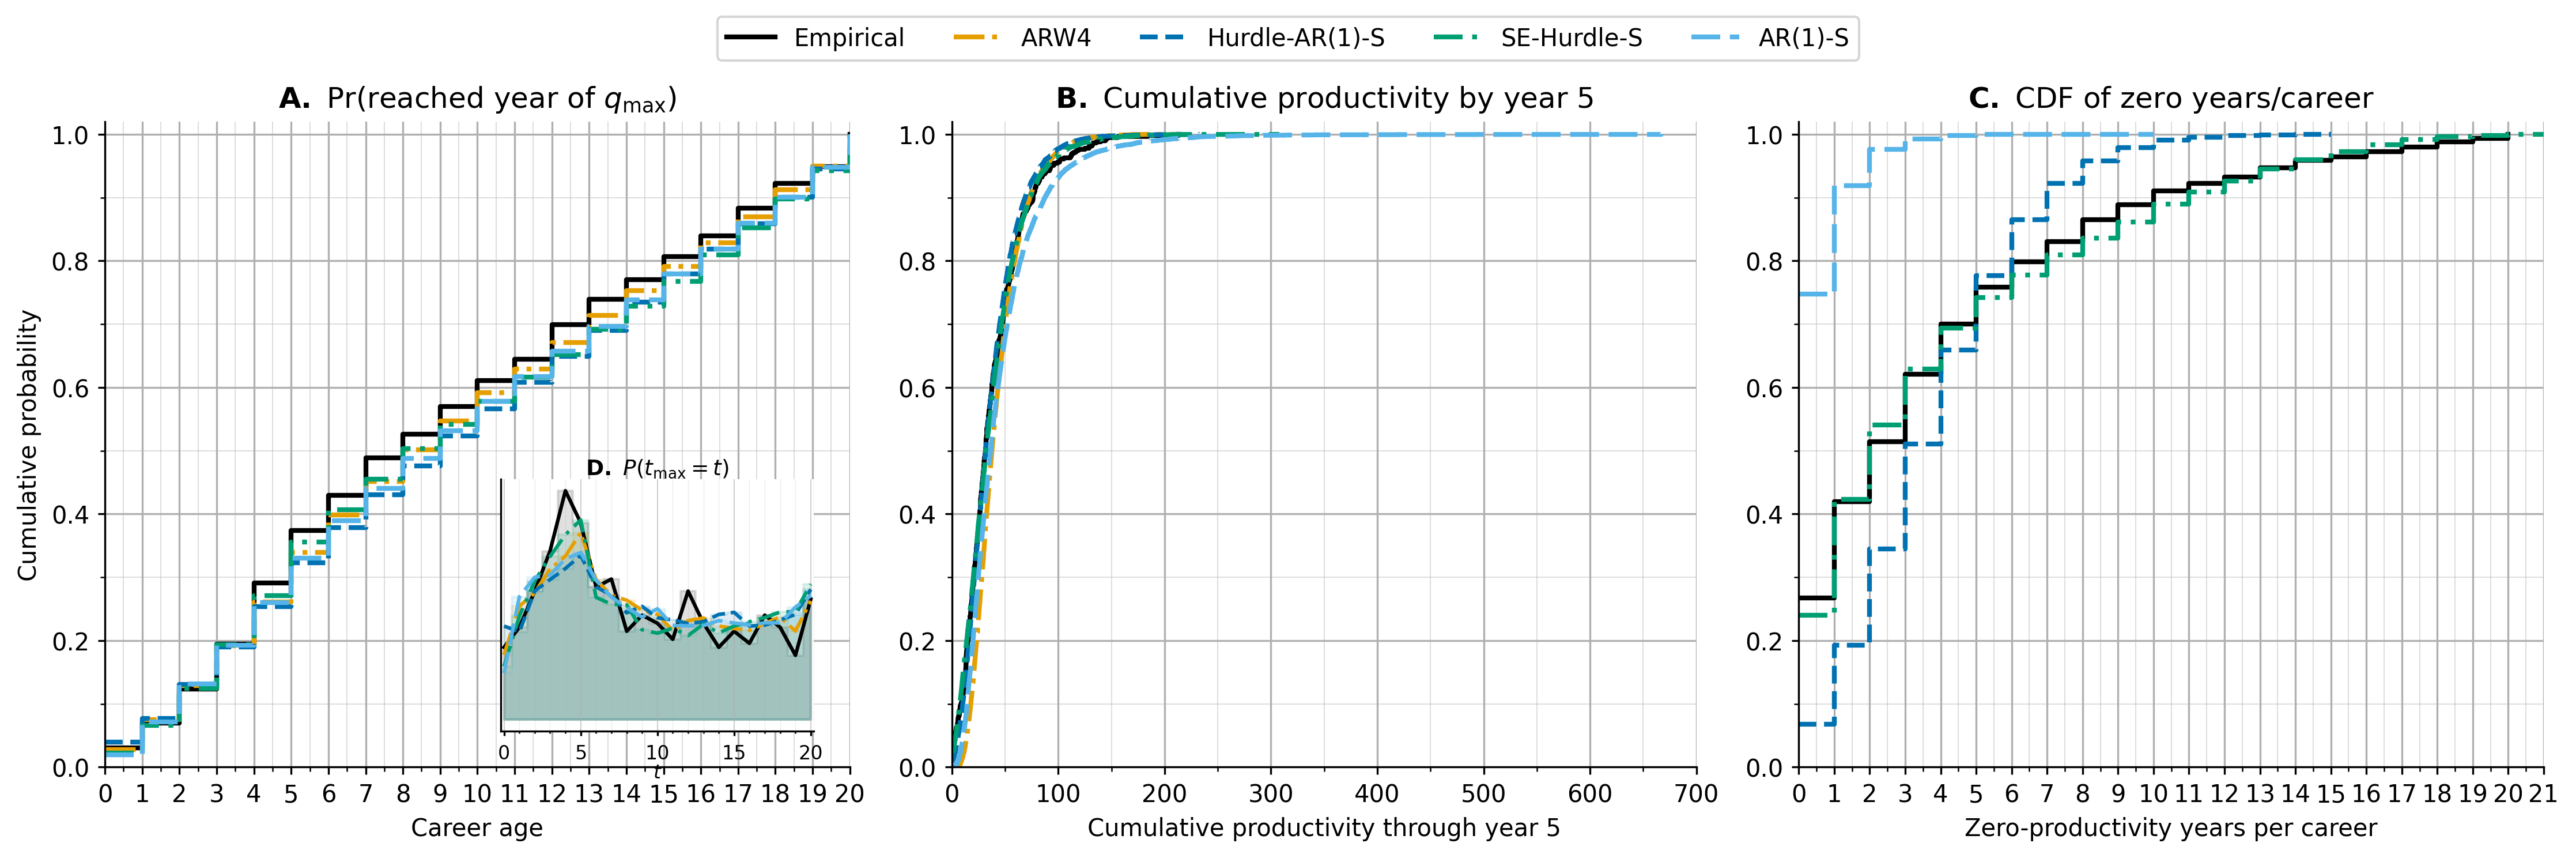
\includegraphics[width=\textwidth]{figures/distributional_cdfs.png}
    \caption{Comparative CDFs. \textbf{A.} The CDF of having already arrived at the year of maximum productivity. \textbf{B.} The CDF of cumulative raw productivity by $t = 5$. \textbf{C.} The CDF of the number of zero years in a career. Inset \textbf{D.} The probability distribution of years of maximum productivity.}
    \label{fig:distributional_cdfs}
\end{figure*}

%%% FIGURE PLACED HERE FOR ORDERING %%%

\subsection{CDFs}
\label{results:CDFs}
In \Cref{fig:distributional_cdfs}, we plotted three cumulative distribution functions: the year of maximum productivity, cumulative productivity by year 5, and number of zero years. 

As shown in \panel{a}, all models match the empirical CDF of year of maximum productivity until after $t=4$, after which all are underestimated. In the inset \panel{d}, we plotted the distribution of years of maximum productivity, which, in line with the trajectories of moments, suggest a slightly wonky temporal displacement. The models estimate $\hat{t}^* = \arg \max_t\; q_t$ one year later than the empirical $t^*$ ($t^* =4, \hat{t}^* =5$). After that, both models roughly trend through the middle of the noisier empirical distribution, before ending higher; this is the source of the underestimated CDFs.

In \panel{b}, we observed close agreement between both models and empirical data. The ECDF is somewhat noisier between 50--100 publications. This is likely a visual artifact of sampling variability.

Lastly, in \panel{c}, SE-Hurdle-S most closely follows the ECDF, while the Hurdle-AR(1)-S CDF is far too steep, suggestive of problems with zero-year modeling. 

AR(1)-S reaches 1.0 far too quickly after starting out too high. In contrast, Hurdle-AR(1)-S starts off far too low, but it too reaches 1.0 prematurely.

ARW4's apparent absence from the plot speaks to an important limitation of that model. It is unplottable because it does not, and cannot, simulate even a single zero year out of its 200,000 simulation-years. Its CDF is degenerate at zero years, where it immediately reaches one and cannot go any further. This is because it draws from a continuous distribution truncated to the nonnegative domain; its draws can only come asymptotically close to 0 (see \Cref{supp:arw4}).

\subsection{Conditional Dropout}
\label{results:conditional_dropout}

In \Cref{fig:conditional_dropout}, we assessed the dynamic of dropout, the transition from a productive state to a zero-productivity state. In our previous GRW and simple AR($p$) approaches, the extensive and intensive margins were compressed into a single prediction. Lacking an explicit inactive state, their conditional dropout probabilities collapse almost immediately to zero.

Hurdle-AR(1)-S began to separate the two margins, but modeled activity using stagewise Bernoulli transitions conditioned only on the preceding activity state. So, an active scholar within a given stage faces similar probability of dropout regardless of productivity magnitude. Its curve remains broadly flat across productivity. These models are included primarily to illustrate the structural consequences associated with their design choices.

\begin{figure*}[!t]
    \centering
    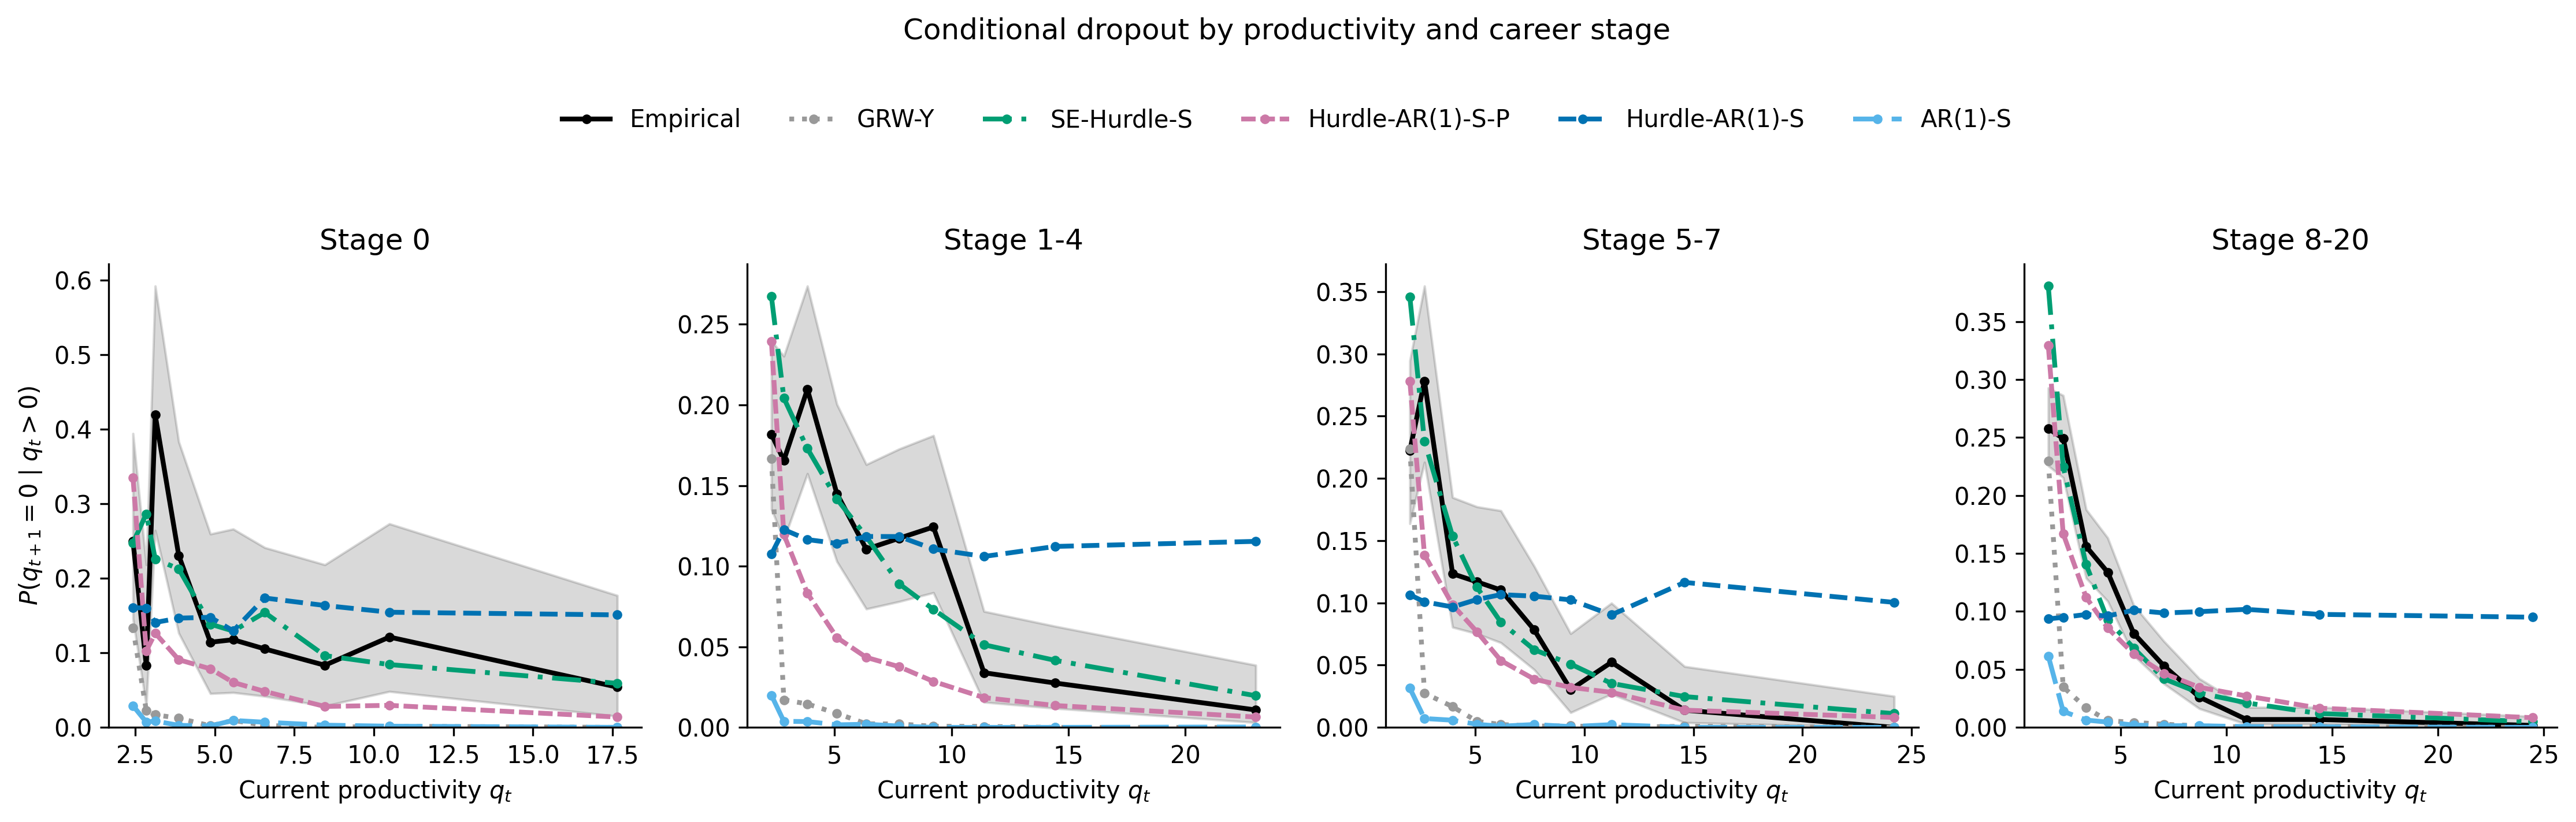
\includegraphics[width=1\linewidth]{figures/conditional_dropout.png}
    \caption{Stagewise conditional comparison of
    $\operatorname{Pr}(b_{t+1}=0\mid b_t=1,q_t)$, the probability that a scholar active in year $t$ enters a zero-productivity state in year $t+1$, conditional on current productivity.}
    \label{fig:conditional_dropout}
\end{figure*}

SE-Hurdle-S reproduces the empirical curves more closely across most stages. It follows both the sharp decline at low productivity and the near-zero dropout probability reached at moderate and high productivity. Unlike Hurdle-AR(1)-S-P, this relationship is not generated by a separate dropout gadget. Rather, it emerges from the extensive-margin equation \eqref{eq:extensive_margin} in which both current productivity and compressed earlier history contribute.

This distinction between the two models is therefore crucial to understanding these results and justifying SE-Hurdle-S. Hurdle-AR(1)-S-P treats dropout as a direct function of $q_t$. SE-Hurdle-S treats $q_t$ as one component of a larger dynamical state. A low-productivity year following a sustained productive history is not equivalent to the same low-productivity year following prolonged decline or inactivity.

Because \Cref{fig:conditional_dropout} conditions on $q_t$ but marginalizes over $H_t$, the SE-Hurdle-S curve represents the average dropout probability across the distribution of histories associated with each productivity bin. Its close agreement with the empirical curve therefore suggests that the history state does not interfere with the well-established current-productivity gradient. Instead, it preserves the marginal current-productivity gradient while allowing additional history dependence within the generative model.

Stage 0 should be interpreted cautiously. It contains only the transition from the first to the second career year, and as a result, empirical estimates are substantially noisier than those of the pooled later stages. The pronounced local spike near low productivity is not necessarily a stable population feature that a monotonic model should be expected to reproduce.

\subsection{Canonical trajectories}
\label{results:canonical_trajectories}

Using the original paper's definition of a canonical trajectory, we found the following:

\begin{figure}[h]
    \centering
    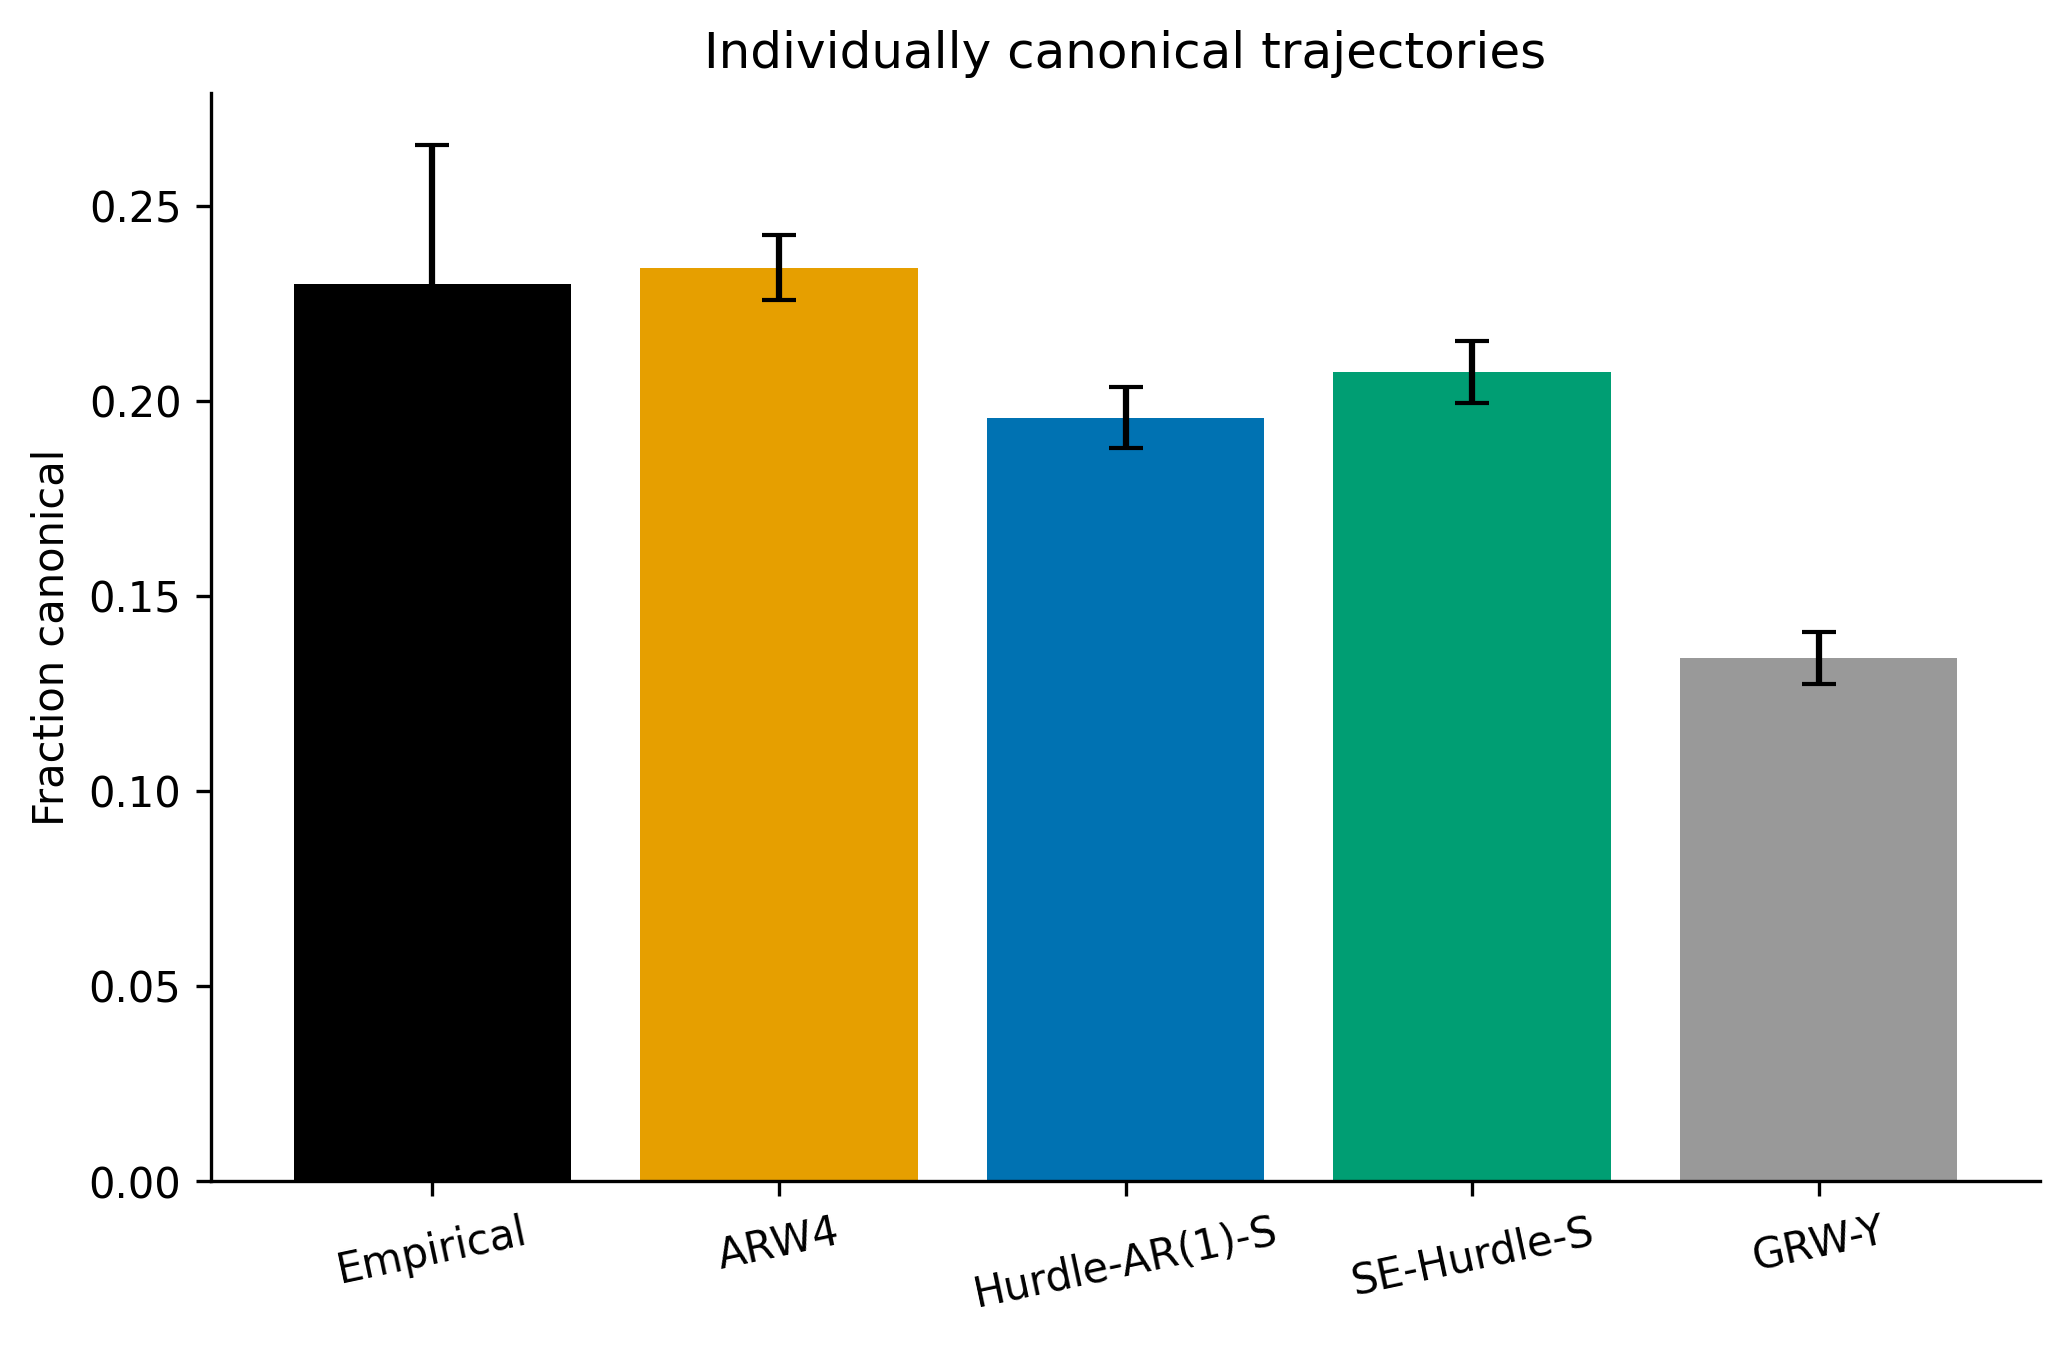
\includegraphics[width=1\linewidth]{figures/canonical_trajectory_fraction.png}
    \caption{Proportion of simulated trajectories classifiable as a canonical trajectory, with error bars.}
    \label{fig:canonical_trajectory_fraction}
\end{figure}

Both hurdle models underestimate, although SE-Hurdle-S does so less severely than Hurdle-AR(1)-S. However, both lie within the empirical uncertainty interval, and their underestimation, while noteworthy, is modest relative to empirical error. GRW-Y severely underestimates the fraction, unsurprising due to its habit of runaway variance.

\subsection{Restart}
\label{results:restart}

In this last diagnostic figure, we appraised the ability of our various models to reproduce the probability of becoming active after a spell of inactivity, conditioned on the length of that spell: $\operatorname{Pr}(q_{t+1}>0 \mid q_{t} = 0, L_t = \ell)$, where $L_t$ is the length, in years, of the current unbroken inactivity run. We identify this as a diagnostic of interest based on existing literature on negative duration dependence of sequential data in studies of employment, for which an established duration dependence literature exists \cite{negativedurationdependence}.

\begin{figure}[H]
    \centering
    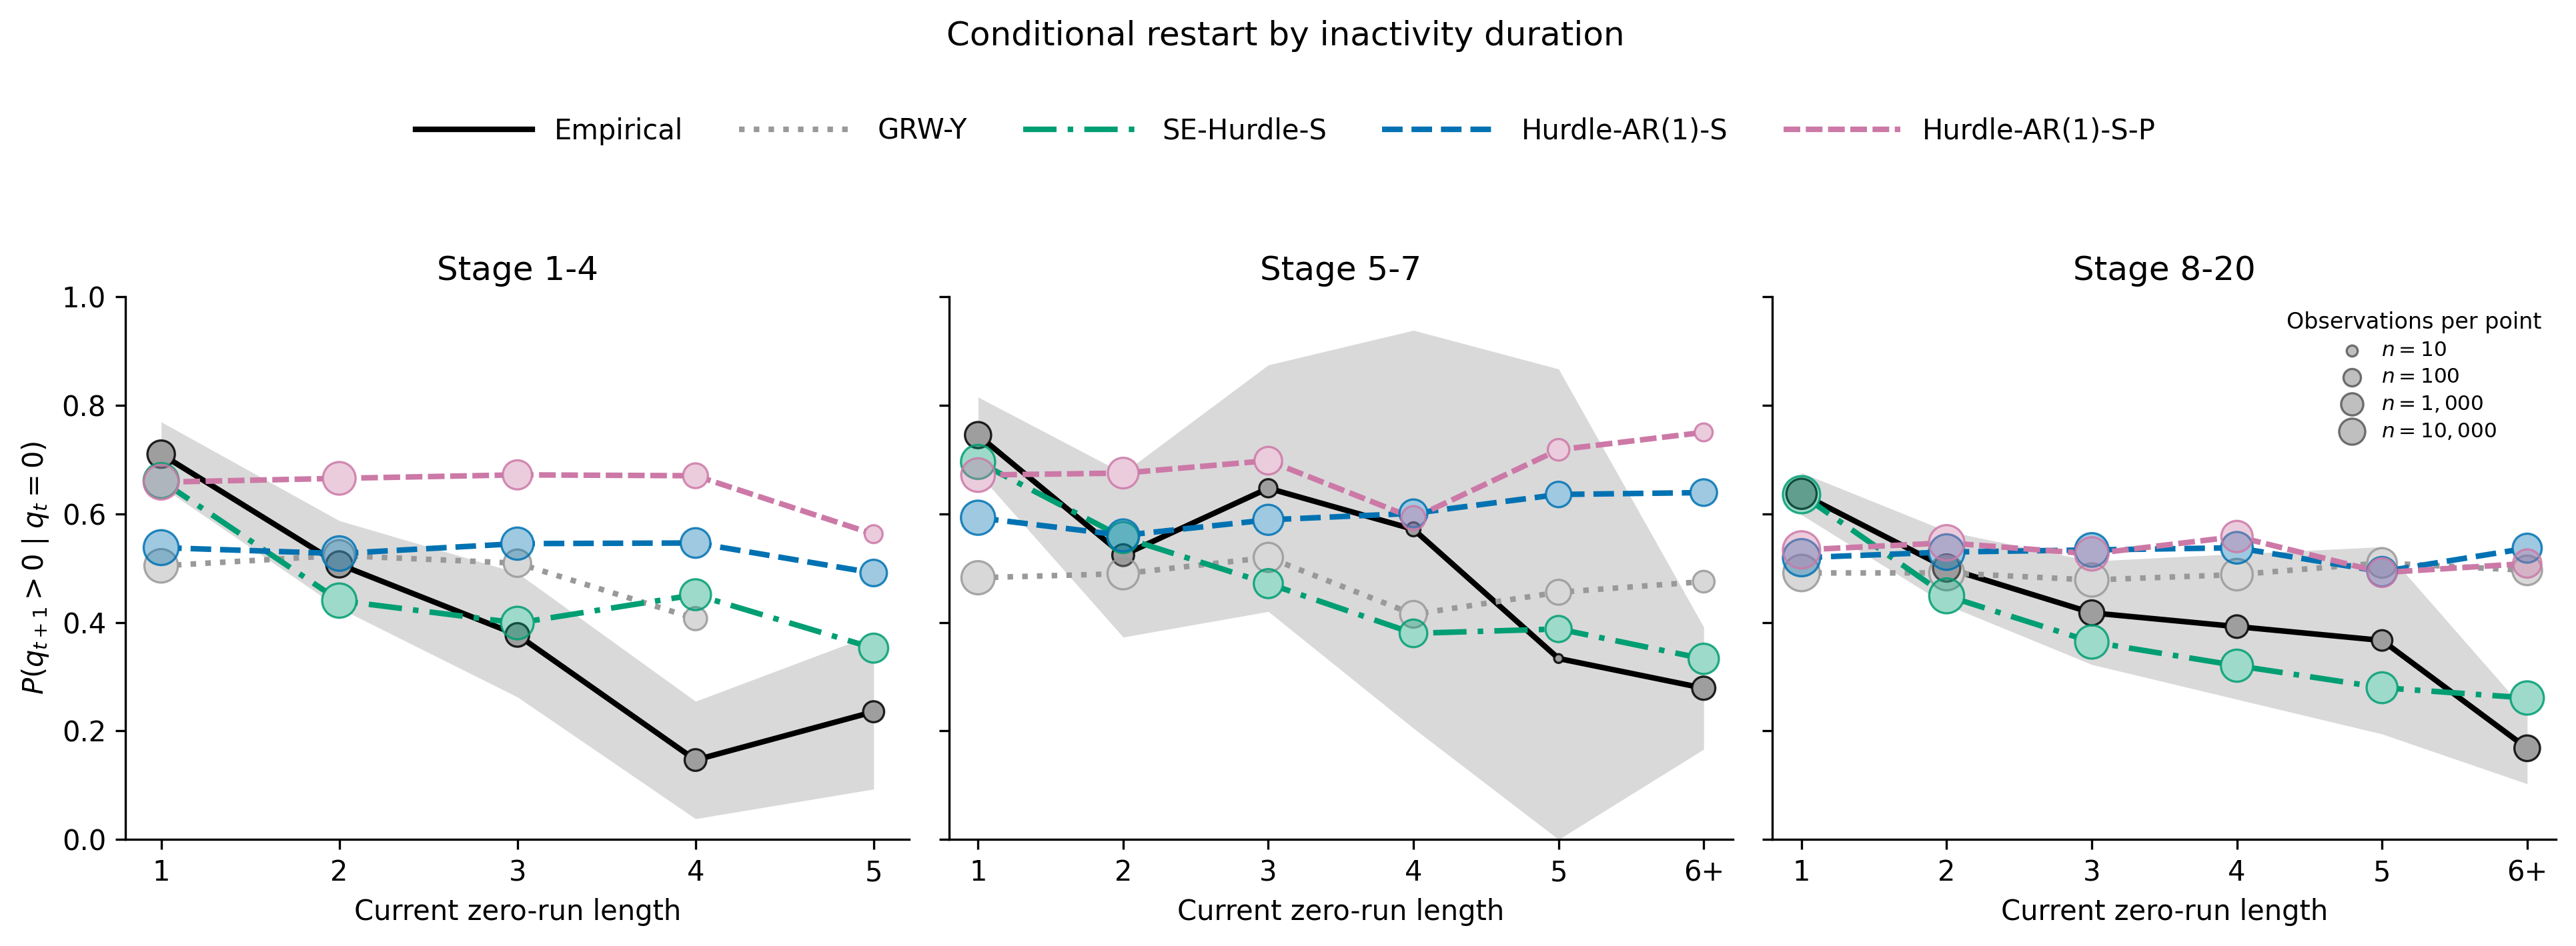
\includegraphics[width=1\linewidth]{figures/conditional_restart_by_zero_run.png}
    \caption{Stagewise trends of simulated and empirical $\operatorname{Pr}(q_{t+1} > 0 \mid q_{t} = 0, L_t = \ell)$, with empirical 95\% CIs. Marker size is a function of observation count.}
    \label{fig:conditional_restart_by_zero_run}
\end{figure}

This characteristic is, essentially, a question of a model's ability to reproduce empirical dynamics that by definition are out of bounds of a first-order Markov process using $q_t$. Across all stages (the first stage is excluded by definition) we saw the negative duration dependence we expected, with mild noise due to varying sample sizes at each model point. The strongest evidence of this comes in Stage 8-20, with an empirical negative trend at all points. While the first two stages have the same endpoint relationship, both have an instance of a positive segment; in both cases the positive segment connects bins with very small sample sizes. In particular, empirical behavior at stages 5-7, with their very small sample size and considerable confidence interval, cannot be mechanistically interpreted without caution. Despite that, it is clear that restart probability tends to decline with zero-run duration, with the clearest evidence in years 8–20.

Hurdle-AR(1)-S has a restart probability defined in its transition matrix, but it is first-order and not conditioned on how long a scholar has been inactive. This leads to a predictable failure mode: after one year, it underestimates restart, and after multiple years, it severely overestimates it, because it is unable to learn the empirical entrenchment dynamic. This is also consistent with its excessively steep 0-year CDF in \Cref{fig:distributional_cdfs}. The next three models are included primarily to illustrate the shared failure mode across multiple model families.

SE-Hurdle-S more closely reproduces empirical dynamics. It struggles somewhat in the first two stages, where bin sizes are quite small, but still broadly resembles the empirical dynamic. In the third stage, it consistently reproduces the empirical trend. This is consistent with the history state allowing restart probabilities to vary with preceding inactivity.

\section{Discussion}
\label{sec:discussion}

SE-Hurdle-S combines an already-developed split-margin hurdle with one simple, decaying history state. Its purpose was not only to outperform past models, but to test the direction proposed by the follow-up to \textit{Scientific Productivity as a Random Walk}. Our results support the broader argument of both papers: stochastic processes agnostic to fixed scholar-level differences can reproduce the major structures of scientific productivity. However, they do not support the elevation of geometric random walks as the particular mechanism responsible.

SE-Hurdle-S provides the best qualitative balance across the diagnostics considered. It reproduces empirical rank persistence, central moment trajectories, zero-year distributions, productivity-dependent dropout, and duration-dependent restart without fixed scholar effects. Its success across both cross-sectional and longitudinal diagnostics suggests that it is not merely trading accuracy in one dimension for accuracy in another. At the same time, it retains several imperfections, particularly excess late-career raw variance and slightly inaccurate peak timing.

The follow-up draft argues that a multiplicative-shock GRW best reproduces cumulative lognormality, Laplace-distributed raw increments, and rank mixing. We find each of these results less identifying than originally proposed. The apparent emergence of Laplace increments was affected by implementation choices documented in the Supplementary Materials. The rank-mixing curve largely follows an analytical property of nested random walks rather than a fitted feature of scientific productivity. Finally, approximately lognormal last-four productivity emerged from nearly every model we tested, including models that failed badly elsewhere. Lognormality is therefore weak evidence for any particular mechanism. A more informative target may be the empirical departure from exact lognormality, particularly in the left tail, which SE-Hurdle-S begins to reproduce and GRW does not.

GRW remains substantially more parsimonious by parameter count. SE-Hurdle-S has 37 nominal parameters, compared with three in the unfitted GRW. However, the GRW's parameter parsimony comes at the expense of explanatory adequacy. SE-Hurdle-S instead offers state parsimony: the entire trajectory before $t-1$ is compressed into one recursively updated variable governed by one global decay parameter.

\subsection{An environmental explanation of \texorpdfstring{$H_t$}{H_t}}
\label{disc:alternate_ht_explanation}

SE-Hurdle-S is self-exciting at the level of observed productivity: earlier values of $q$ contribute to a persistent state $H_t$ that predicts later activity and output. This statistical dependence does not establish that publications themselves causally produce later publications. Instead, $H_t$ may partially summarize persistent but unobserved features of a scholar's productive environment.

One candidate is scientific labor. Zhang et al.\ find that the greater productivity of faculty at prestigious institutions is associated with greater access to funded graduate and postdoctoral researchers. In disciplines with research-group norms, funded labor predicts larger groups and greater group productivity, while the productivity of individual group members changes little with prestige \cite{laboradvantages}.

Research-group size, active collaborations, funding, and project pipelines are not directly encoded in our trajectories, but they are likely to persist across years and leave a signature in earlier productivity. Two scholars with identical $q_t$ may therefore have different future productivity because one maintains a larger group or stronger project pipeline. In this interpretation, the failure of $q_t$ as a complete first-order state does not imply that old papers directly yield new ones. Rather, past productivity may reveal persistent productive capacity not contained in the current count alone.

This connection also clarifies decaying history. Scientific labor and collaboration structures have inertia, but students graduate, postdocs leave, grants expire, and projects conclude. Their effects may persist while gradually losing predictive value, consistent with the role assigned to $H_t$. The labor-advantage results do not, however, identify an exponential kernel or establish our fitted $\rho$, and $H_t$ may also proxy funding, prestige, topic, health, teaching load, or other persistent influences.

\subsection{Path-dependent stochasticity and cumulative advantage}
\label{disc:path_dependence}

The follow-up draft contrasts Shockley's stable individual traits with individualized yearly shocks. SE-Hurdle-S introduces a third possibility:
\begin{center}
    fixed talent\\
    \textit{vs.}\\
    memoryless stochasticity\\
    \textit{vs.}\\
    path-dependent stochasticity.
\end{center}

Scientists may be identical with respect to the model's fixed parameters without remaining identical with respect to their accumulated states. Early stochastic differences alter $H_t$, which then affects later activity and productivity. The resulting heterogeneity is persistent but revisable: history matters, but its influence decays.

This framing also better reflects the draft's proposed multiplicative accumulation of opportunities. In the GRW,
\[x_t=\gamma_t x_{t-1},\]
the shocks are independent. The process accumulates multiplicatively, but contains no explicit representation of resources, institutional reinforcement, prolonged inactivity, or conditional dropout and restart. SE-Hurdle-S does not directly observe opportunity either, but its persistent history state provides a statistical representation compatible with temporary persistence in productive capacity. In that sense, the model is closer to the theoretical spirit of cumulative advantage than the GRW itself.

\subsection{Limitations and further development}
\label{disc:lims}

Our main limitation is the empirical sample size. The analysis uses $n^{\mathrm{emp}}=591$ complete trajectories, compared with $n^{\mathrm{sim}}=10{,}000$ simulated careers. Rare outcomes are therefore represented noisily in the empirical data, producing irregular upper tails and wide confidence intervals in sparsely occupied conditional bins. This is especially visible above $q_t=30$ and at long zero-run lengths in the earlier career stages.

The data are also limited to computer science. We therefore cannot assume that the fitted decay rate, history effects, or inactivity dynamics generalize to fields with different publication and collaboration norms. A direct next step is to fit SE-Hurdle-S separately across disciplines and compare $\rho$, the extensive- and intensive-margin history coefficients, rank persistence, and zero-state dynamics. If $H_t$ partly represents research-group capacity, its effects should be stronger in fields where faculty commonly lead and publish with research groups. Adding direct measures of group size and funded labor would further clarify whether the apparent self-excitation reflects accumulated organizational capacity or an autonomous effect of publication history.

Additionally, although the predictive-benefit tests were performed with held-out metrics, the majority of diagnostics were not. SE-Hurdle-S was fitted and evaluated largely on the same 591 careers.

SE-Hurdle-S is the result of iterative model development in response to failure modes and testing of data. Although we have taken care to challenge and justify for our results and architecture decisions, the possibility of researcher-driven overfitting even without scholar-specific parameters is not eliminated.

Simulation intervals generally reflect simulation variation conditional on fitted parameters, not uncertainty in the estimated coefficients and $\rho$.

Restricting analysis to 591 complete trajectories may select for scholars with longer or more observable careers.

The CK test was performed over four positive-productivity bins and the exact-zero state, so it can only be interpreted in that space; further testing over different bins is required to generalize more.

Finally, the positive margin is continuous even though publication productivity has a discrete lower limit. The current simulations can generate arbitrarily small positive values that are not empirically meaningful. Future versions should compare the present continuous specification with a positive distribution truncated at the empirical single-unit boundary, or with an explicitly discrete count model.

\section{Conclusion}
\label{sec:conclusion}

We design and test SE-Hurdle-S, a split-margin, self-exciting hurdle model that provides the best qualitative balance across the diagnostics considered. Its success supports the central argument of both \textit{Scientific Productivity as a Random Walk} and its follow-up draft: stochastic career dynamics can reproduce persistent differences in scientific productivity without fixed scholar-level heterogeneity. However, our results do not support the geometric random walk as the particular mechanism responsible.

GRW reliably produces cumulative lognormality, but this property emerged from nearly every model we tested and is therefore non-identifying. Its apparent reproduction of Laplace-distributed increments and empirical rank mixing also provides weaker evidence than initially proposed. By contrast, SE-Hurdle-S generates Laplace-like raw increments without Laplace innovations and closely reproduces empirical rank persistence alongside the principal moment, zero-year, dropout, and restart dynamics.

The model introduces a distinction between identical parameters and divergent individual histories. Scientists may begin as exchangeable within the model while becoming dynamically unequal through path-dependent stochasticity. The history state may represent accumulated opportunity, persistent productive capacity, or unobserved environmental resources, although the present analysis cannot distinguish among these mechanisms. Our findings, then, reinforce the stochastic alternative to Shockley's fixed-trait account within computer science while motivating cross-disciplinary tests of history dependence and its possible labor-based foundations.

\bibliographystyle{plain}
\bibliography{references}

\clearpage

\onecolumn
\begin{center}
    {\Large\bfseries Supplementary Materials}
\end{center}
\vspace{1em}


\setcounter{section}{0}
\renewcommand{\thesection}{Supp. \arabic{section}}

\section{More on held-out models}
\label{supp:held_out_rank_mixing}
We tested a flexible nonparametric kNN first-order Markov model, one allowed to learn nonlinear, age-specific, empirical transitions while using only:
\[
    (t, q_t, \mathbbm{1}\{q_t>0\}).
\]
Despite all its flexibility, its rank persistence collapses to $\hat{\rho}(R_0, R_{20}) = 0.000,\; 99\% \text{ CI }[-0.089,0.102]$, while the empirical $\rho(R_0,R_{20})= 0.202$. As noted in the results of AR(1), rank mixing is very similar to empirical after one year, but quickly diverges afterwards:
\begin{figure}[H]
    \centering
    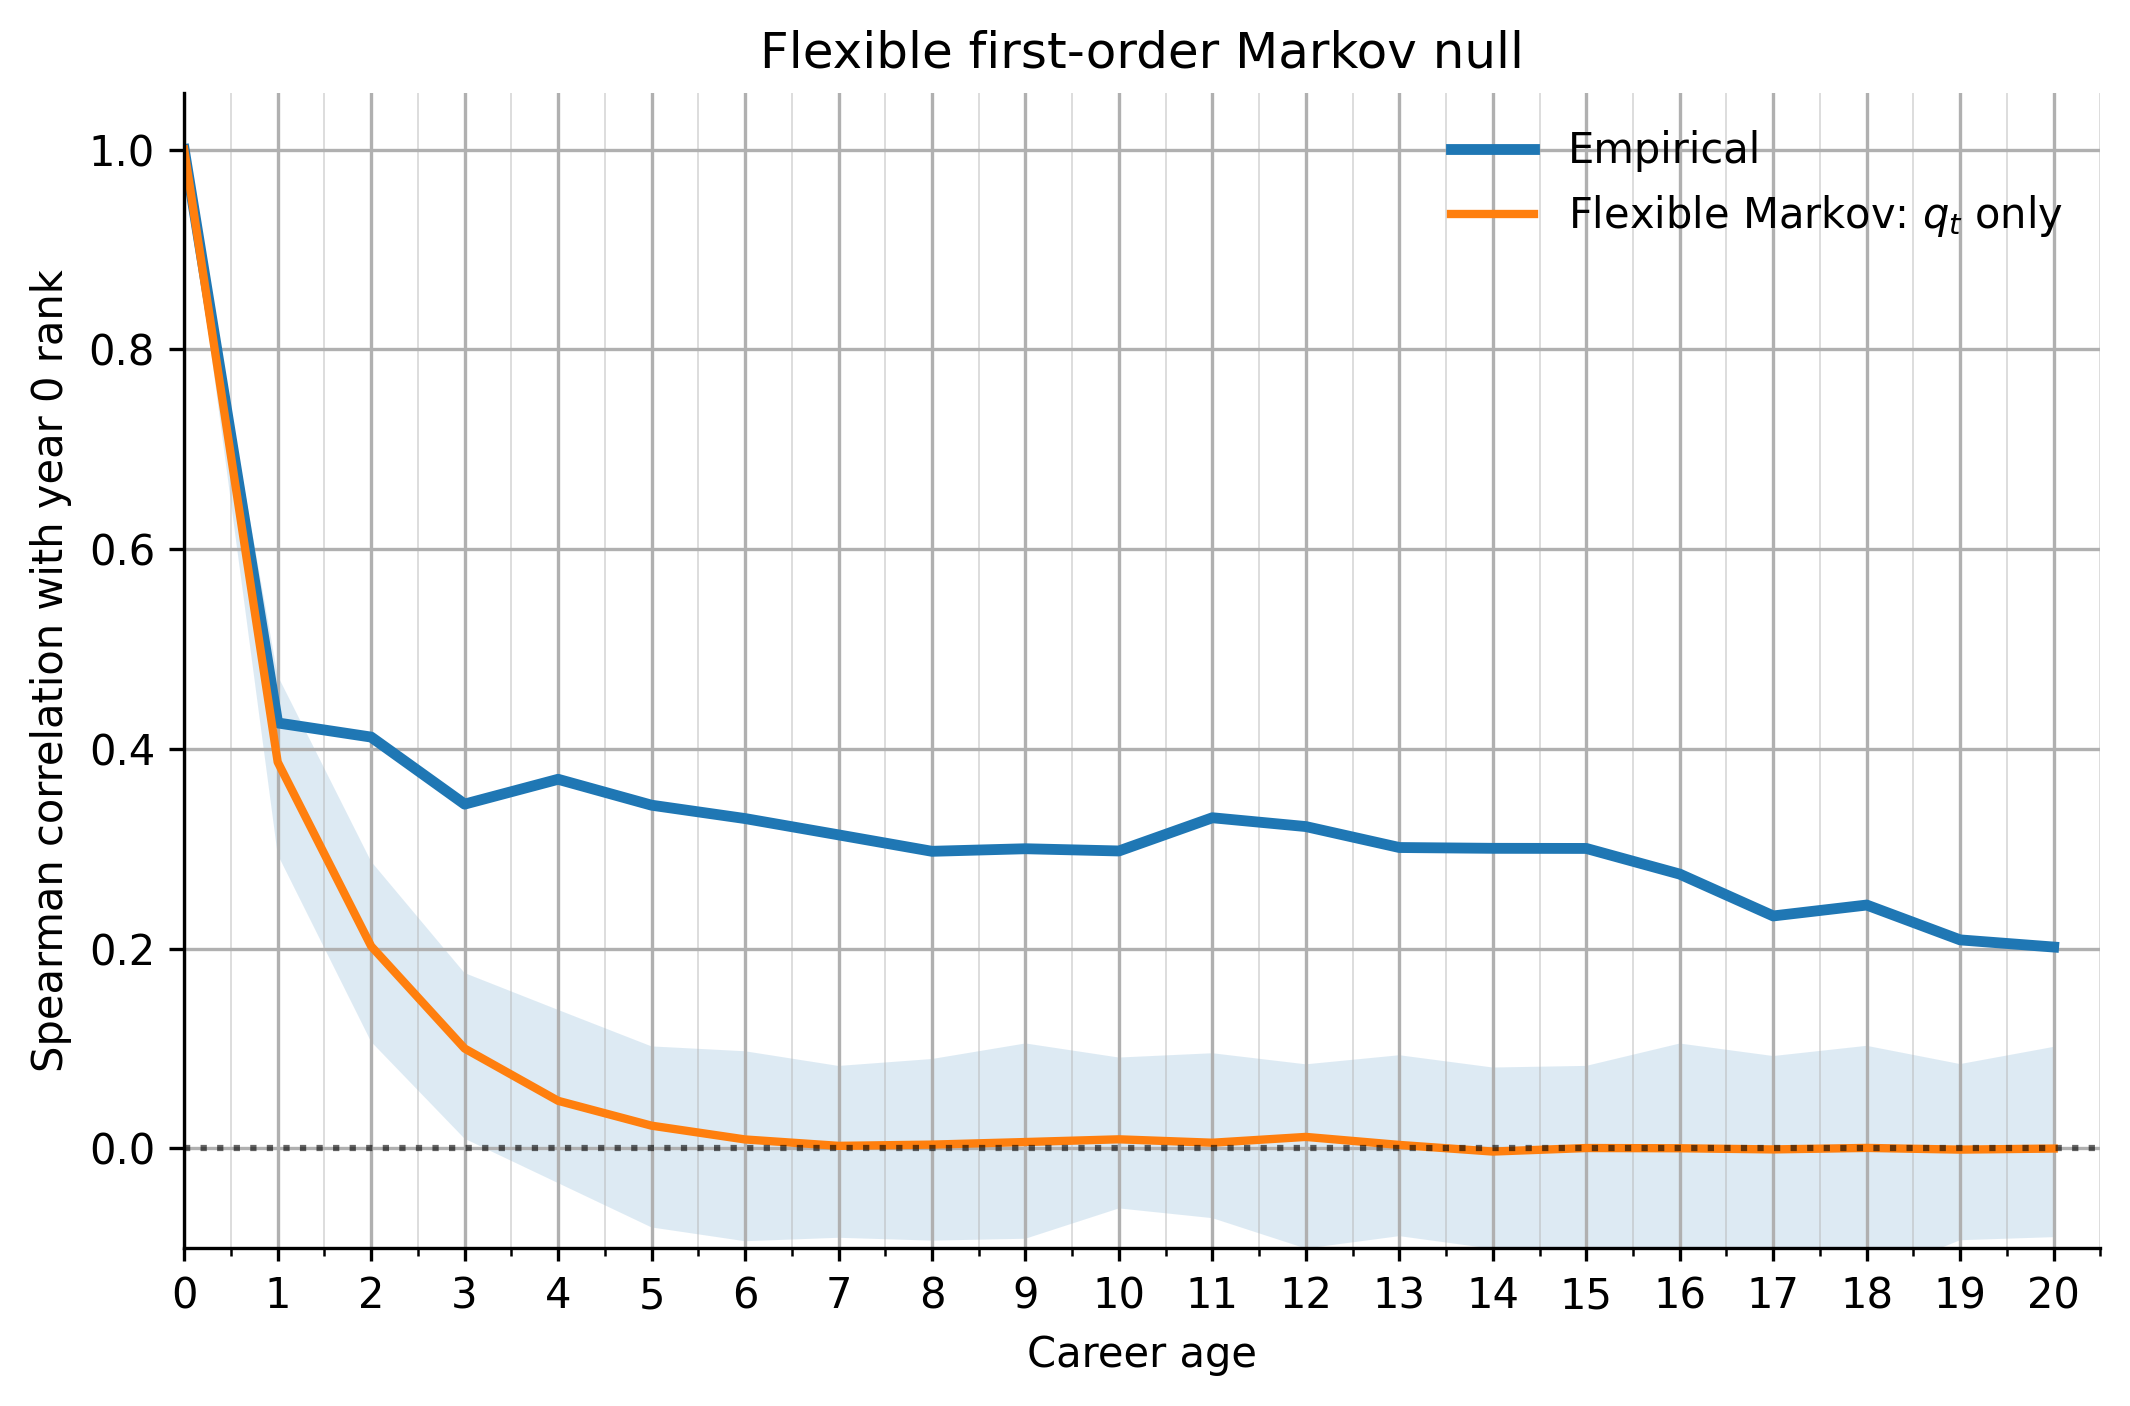
\includegraphics[width=0.7\linewidth]{figures/knn_markov_rank_mixing.png}
    \caption{Rank-mixing of the nonparametric first-order Markov model. Close alignment in the first year collapses to zero by year 8.}
    \label{fig:knn_markov_rank_mixing}
\end{figure}
This is the same trajectory shape as every tested model before SE-Hurdle-S. Evidently, knowledge of $(t, q_t, \mathbbm{1}\{q_t>0\})$ is enough to last one year but not anything else beyond that. 

\section{Diminishing returns of higher-order AR(\textit{p})}
\label{supp:arp_diminishing}

Extending the stagewise autoregressive model beyond the first order produced a clear pattern of diminishing returns. Relative to AR(1)-S, AR(2)-S reduced held-out Gaussian loss by approximately 4.8\% and held-out log-scale RMSE by 6.2\%. AR(3)-S yielded additional improvements of only 1.5\% and 1.8\%, respectively, while AR(4)-S improved the same metrics by less than 1\%. 

\begin{figure}[H]
    \centering
    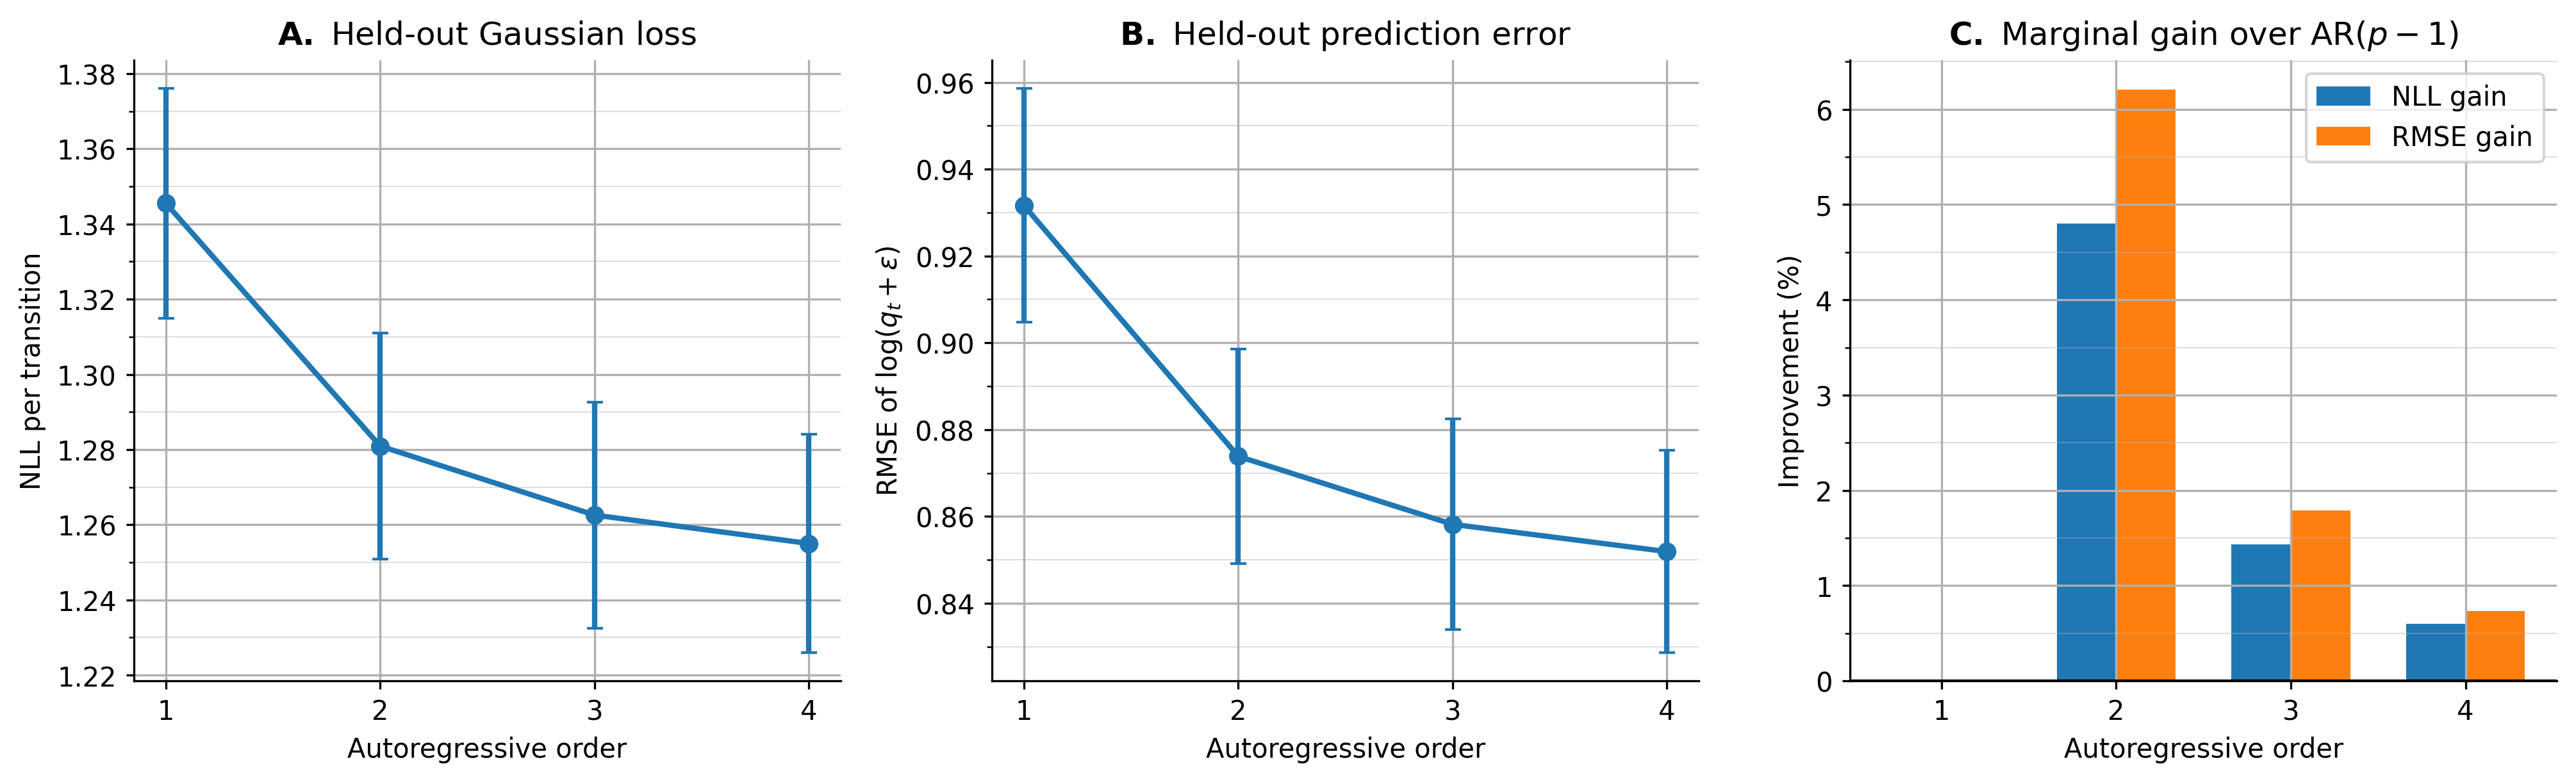
\includegraphics[width=1\linewidth]{figures_ar_p/predictive_diminishing_returns.png}
    \caption{Diminishing returns brought about by increasing $p$. There is a clear 'elbow' at AR(2) across most metrics.}
    \label{fig:predictive_diminishing_returns}
\end{figure}

Thus, most of the predictive benefit available between orders one and four was obtained from the first additional lag. Higher orders also reduced residual serial dependence and slowed the loss of rank persistence, demonstrating that productivity history beyond $q_t$ contains relevant information. 

\begin{figure}[H]
    \centering
    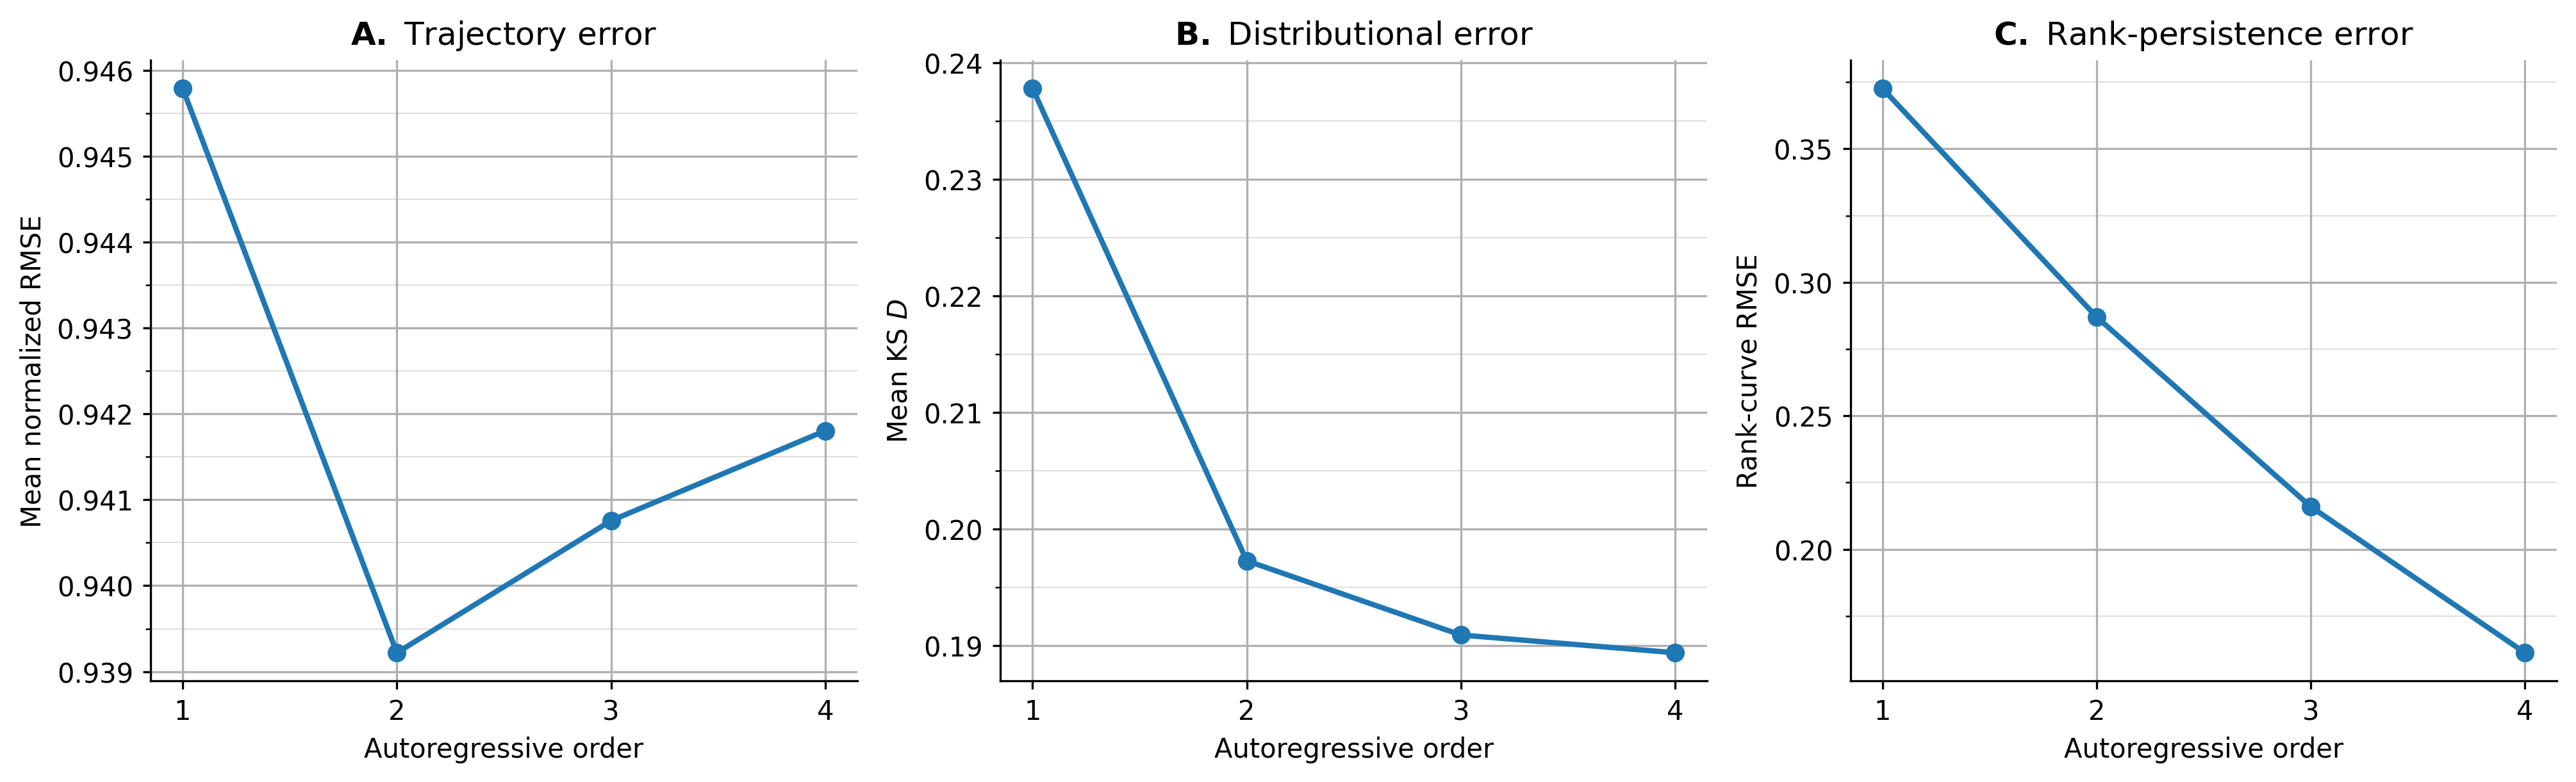
\includegraphics[width=1\linewidth]{figures_ar_p/generative_diminishing_returns.png}
    \caption{Generative diminishing returns. The only metric in which we did not see the characteristic shift at AR(2) is rank mixing, and what we observed in trajectory error is far more severe than just an elbow.}
    \label{fig:generative_diminishing_returns}
\end{figure}

These improvements, however, did not repair the principal generative failures of the model family. All four orders overestimated mean productivity, underestimated cross-sectional log variance, generated far too few zero years, and lost empirical rank persistence too rapidly. Aggregate trajectory error was minimized at $p=2$ and worsened slightly thereafter, while distributional error changed little beyond the second order. Increasing autoregressive order therefore exchanged a linear increase in parameter count for progressively smaller predictive gains and no qualitative correction of the empirical dynamics. 

\begin{figure}[H]
    \centering
    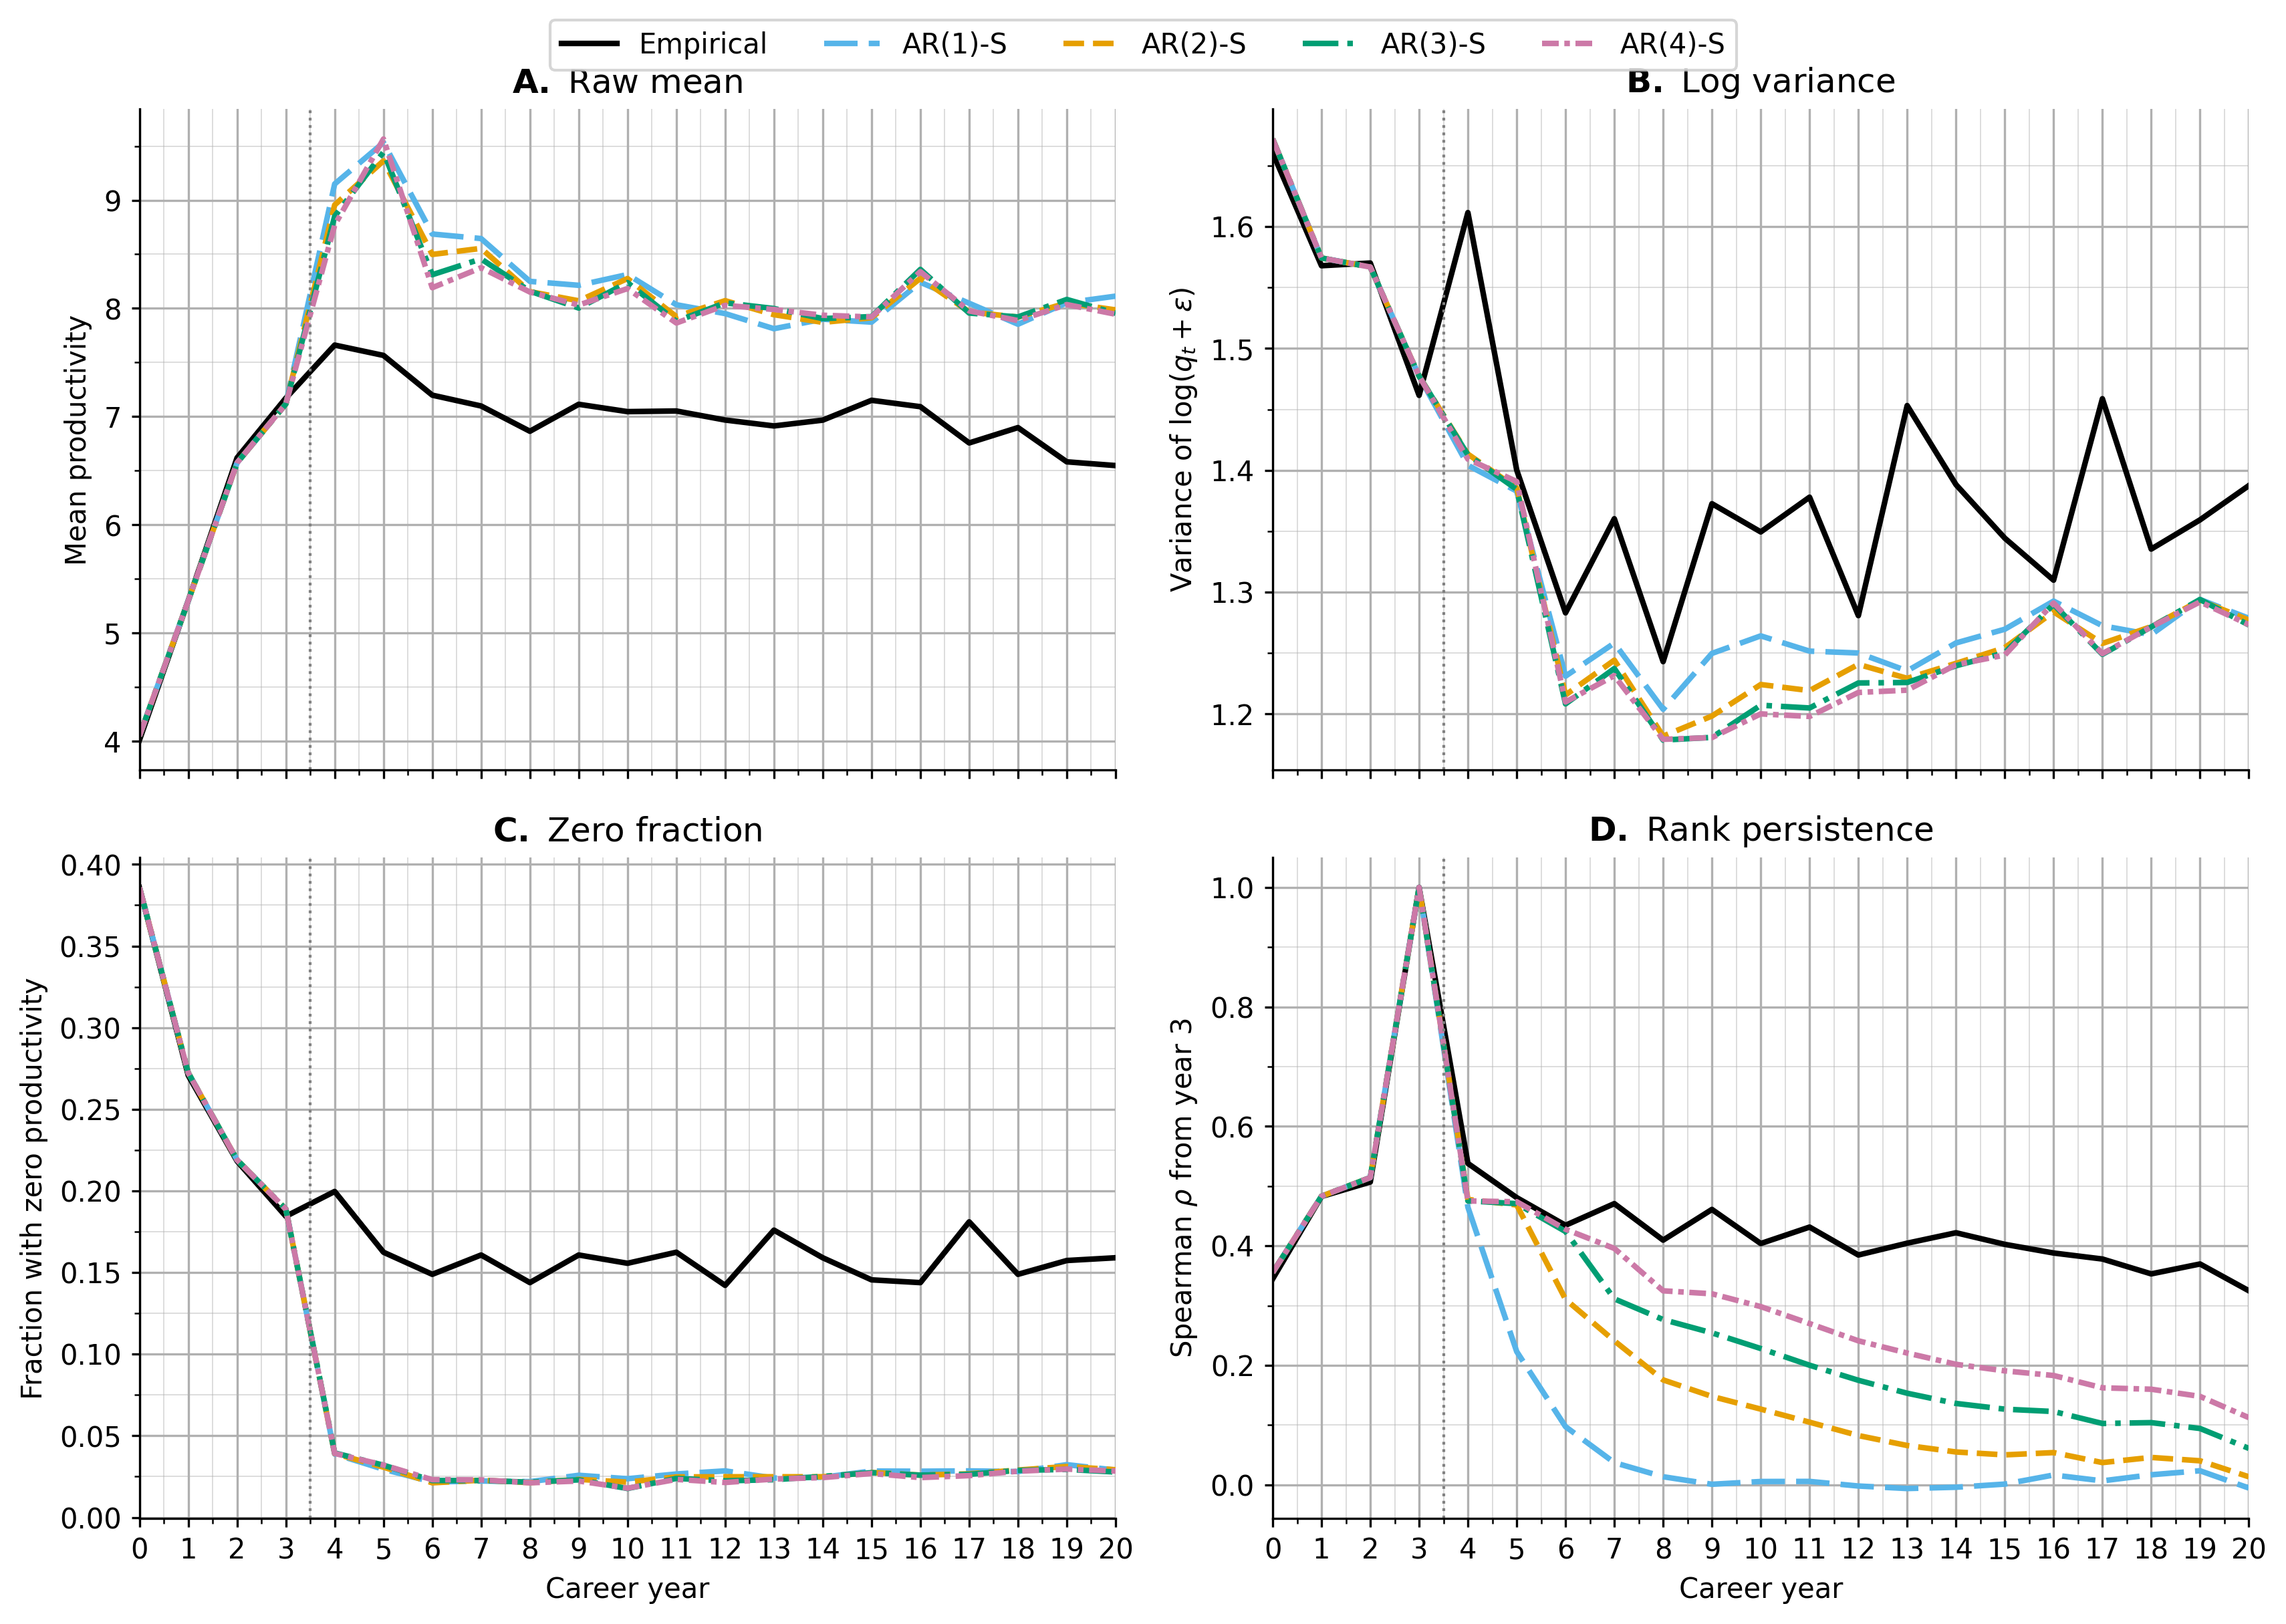
\includegraphics[width=1\linewidth]{figures_ar_p/generative_trajectory_comparison.png}
    \caption{Comparison of diagnostic trajectories. All ARs, regardless of improvement in other areas, show central shortcomings inherent to their structure, not their order.}
    \label{fig:generative_trajectory_comparison}
\end{figure}

We interpret this not as evidence against temporal dependence, but as evidence that a finite vector of recent productivity values is an inefficient state representation. The remaining discrepancies instead motivate an explicit hurdle process and a parsimonious history-dependent state capable of representing longer-run productive momentum.

\section{The impact of history on SE-Hurdle-S}
\label{supp:history_impact_on_se_h_s}
We demonstrated above that, generally speaking, history has predictive value. We come back to this potential as realized in this model specifically, and retrieve the stagewise impact coefficients described below:

\begin{table*}[!h]
\centering
\caption{Stagewise history effects. History-coefficient estimates are
scholar-bootstrap medians with percentile 95\% confidence intervals.
Intercepts are full-sample estimates shown for reference.}
\label{tab:history_effects}

\begin{tabular}{||c| c| c| c| c| c| c||}
\hline
Stage
& $\hat{\delta}_s$ & 95\% CI & $\hat{\alpha}_s$ & $\hat{d}_s$ & 95\% CI & $\hat{a}_s$ \\
\hline
$1$--$4$
& 0.629 & $[0.453,\,0.815]$ & $-0.410$ & 0.238 & $[0.190,\,0.279]$ & 0.790 \\
\hline
$5$--$7$
& 1.301 & $[1.010,\,1.594]$ & $-0.671$ & 0.400 & $[0.337,\,0.464]$ & 0.368 \\
\hline
$8$--$20$
& 1.380 & $[1.220,\,1.565]$ & $-1.164$ & 0.488 & $[0.450,\,0.527]$ & 0.051 \\
\hline
\end{tabular}
\end{table*}

The unrestricted bootstrap estimates are positive in all stages, so the fitted positive history effects are not solely from the imposition of a nonnegativity constraint.

Based on this data, given a single-unit increase in $H_t$, the multiplicative impact on the odds of activity is (stagewise):
\[
e^{0.629} = 1.88, \quad e^{1.301} = 3.67,\quad e^{1.380}=3.97,
\]
and the multiplicative impact of the same increase in $H_t$ on the intensive margin is:
\[
e^{0.238} = 1.27, \quad e^{0.400} = 1.49, \quad e^{0.488} = 1.63.
\]
This suggests a dynamic rather more than simple autoregressive persistence: the impact of productivity history becomes \emph{greater} later in the career. At the same time, however, stage intercepts actually strictly decline in both margins, suggesting early-career activity has a strong common baseline, while later-career activity grows increasingly conditional on accumulated history.

Several independent tests show that the history term has predictive value, including an empirical mean two-step CK error of 0.1280 against 0.0572 in a test of first-order sufficiency of $q_t$, corresponding to a p-value of $0.0000999$.

\section{Hawkes vs. SE-Hurdle-S}
\label{supp:hawkes_v_se_h_s}

SE-Hurdle-S is self-exciting in the broad sense that earlier observed
productivity positively affects the conditional distribution of later
productivity. It is not a Hawkes process.

A Hawkes process is formulated as a continuous-time point
process with a conditional event intensity increased by previous
events. SE-Hurdle-S instead operates in discrete annual time and models aggregate productivity through two linked components: a Bernoulli activity equation and a conditional positive-output equation.

The models differ in several specific respects:

\begin{itemize}
    \item SE-Hurdle-S models annual productivity totals rather than
    individual event times.
    \item Earlier productivity enters both margins of SE-Hurdle-S:
    through $\delta_s H_t$ in the activity equation and through
    $d_s H_t$ in the positive-output equation.
    \item The history state $H_t$ is a normalized exponentially
    weighted average of past $\log(1+q)$ values. A conventional Hawkes excitation term is instead formed by summing event-specific kernel contributions to a conditional intensity.
    \item Individual publications do not act as separately timed
    triggering events. Their annual aggregate contributes to the
    subsequent history state.
    \item The fitted parameter $\rho$ controls the relative decay of
    historical weights. It is not a Hawkes branching ratio and does not measure the expected number of future publications caused by one publication.
    \item The history effect is transformed differently in the two
    margins. In the activity equation, the logistic link bounds the
    resulting probability between zero and one. In the positive-output equation, $d_sH_t$ enters linearly on the log scale and therefore acts multiplicatively on positive productivity.
\end{itemize}

The analogy is architectural, not exact. Both model
classes allow earlier activity to affect a later conditional
distribution and permit that influence to decay over time. SE-Hurdle-S adapts that general idea to a discrete-time hurdle
autoregression for annual productivity counts.

\subsection{History dependence and exponential memory}
\label{supp:support_of_se}

SE-Hurdle-S depends not only on immediately preceding productivity but also on compressed prior history $H_t$. This construction places SE-Hurdle-S in a class of self-exciting models where the present distribution depends on the observed history of the process. 

In the Hawkes process architecture, self-excitation is introduced through a conditional intensity:

\begin{equation}
\lambda(t\mid\mathcal H_t) = \nu+\sum_{j:t_j<t}g(t-t_j),
\label{eq:hawkes_history}
\end{equation}

where $g$ is a trigger determining how the influence of each prior event declines with elapsed time \citep{hawkes1971spectra,reinhart2018review}. The exact kernel controls whether dependence is concentrated in the recent past or persists over longer intervals. SE-Hurdle-S is not a Hawkes process (see \Cref{supp:hawkes_v_se_h_s}), but the shared idea is that past activity modifies the current conditional distribution, and that older observations matter less than recent ones.

A close methodological precedent is the self-exciting hurdle model of Porter and White \citep{porter2012selfexciting}. Porter and White separately model the probability of a nonzero event count and the distribution of the positive count, while allowing both components to depend on a history-based process,

\begin{equation}
S_t =
\sum_{s<t}E_s\alpha_s g(t-s).
\label{eq:shot_noise_history}
\end{equation}

Their architecture demonstrates that hurdle layering and self-exciting history dependence can be combined within the same discrete model. The analogy to SE-Hurdle-S is architectural, not exact. 

$H_t$, then, can be understood as a normalized geometrically weighted distributed lag, an exponentially weighted history state, or a discrete exponentially decaying memory kernel. In continuous evolution equations, a similar memory operator is given by

\begin{equation}
(Kv)(t) = \int_0^t k(t-s)v(s),ds, \qquad k(z)=\lambda e^{-\lambda z},
\label{eq:volterra_memory}
\end{equation}

a Volterra convolution with an exponentially decaying kernel \citep{volterrakernel}. Under observations with regular spacing, exponential decay in continuous time corresponds to geometric decay in discrete time through

\[
\rho=e^{-\lambda\Delta t}.
\]

Our normalization in $H_t$ is an important distinction. Rather than representing the accumulated mass of past productivity, $H_t$ represents its exponentially weighted average. It remains on the scale of $log(1+q)$ and does not grow structurally with the number of observed career years.

The parameter $\rho$ controls the persistence of historical influence. Observations separated by $k$ additional years have relative weight $\rho^k$, giving the memory half-life

\begin{equation}
h_{1/2}=
\frac{\log(1/2)}{\log\rho}.
\label{eq:memory_half_life}
\end{equation}

Values of $\rho$ near zero concentrate the history term on the recent past, while values near one distribute weight more evenly across the observed career. Because $q_{t-1}$ enters the margins separately, $H_t$ is calculated only through $t-2$. The model thereby distinguishes immediate autoregressive dependence from the residual influence of longer productivity history.

This exponential kernel is parsimonious and recursively computable, but it is also restrictive. It assumes that historical influence declines smoothly and geometrically, and therefore cannot independently represent multiple memory scales, delayed effects, or particular past events whose influence persists without monotonic decay. The literature supports exponential weighting as a standard and tractable representation of history dependence, not as the uniquely appropriate memory structure for scientific productivity.


\section{Rank-mixing in GRWs}
\label{supp:grw_rankmixing}
As discussed, one exciting property that supported the use of GRWs was its superficial ability to rank-mix like empirical data. This turns out to be the result of an analytical relationship. Because exponentiation is a monotonic function, it follows that, at some time $t$ and for some individual $i$, $\operatorname{rank}(x_{i,t}) = \operatorname{rank}(z_{i,t})$. 

Logically, for any year $s<t$, it must be that
\[
    z_{i,t} = z_{i,s} + \sum_{k=s+1}^t \epsilon_{i,k}.
    \label{eq:sumwithk}
\]
For two normal random variables,
\begin{equation}
    \operatorname{Corr}(z_s, z_t) = \frac{s\sigma^2}{\sqrt{s\sigma^2t\sigma^2}} = \sqrt\frac{s}{t}.
    \label{eq:covariance}
\end{equation}
Under assumptions of equal variance and independent-increment assumptions.
Using the Spearman bivariate normal correlation:
\begin{equation}
    \hat{\rho}_S(s,t) = \frac{6}{\pi} \arcsin{\bigg[\frac{1}{2}\sqrt\frac{s}{t}\bigg]}.
    \label{eq:spearman_est_of_pearson}
\end{equation}
For instance, $\hat{\rho}(1,20)$, the correlation between the ranks of year 1 and year 20, is $\approx 0.214$. Of note, the value of $\hat{\rho}(s,t)$ at any point is independent of the model parameters $(x_0, \mu, \sigma^2)$.

While this property is exact for once-fitted GRWs and only approximate for anything else, it appears to remain strongly applicable; the rank mixing curve of GRW-Y and GRW-S have a shape highly similar to that of the draft GRW and all three are highly similar to the actual plotted curve of that analytical relationship.

\section{Past models}
\label{supp:past_models}

The present model emerged from a longer sequence of increasingly constrained random-walk, autoregressive, and hurdle models. We summarize the most informative members of that sequence here. The purpose is not to reproduce every intermediate model or auxiliary gadget tested during development, but to establish the principal baselines against which the present model should be understood. Together, these models trace the progression from an unconstrained multiplicative random walk, through stagewise mean reversion, to an explicit separation of the extensive and intensive margins of scientific productivity.

Throughout, \(q_{i,t}\geq 0\) denotes the productivity of scholar \(i\) at career age \(t\), and

\[
    z_{i,t}=\log(q_{i,t}+\eta)
\]

denotes shifted log productivity, with \(\eta>0\) included so that zero-productivity years remain well-defined. The function \(s(t)\) maps career age to one of the four empirically defined career stages. Unless otherwise stated, all models are scholar-agnostic: their parameters vary across years or career stages, but not across individual scholars.

\subsection{ARW4}
\label{supp:arw4}

ARW4 is a four-stage autoregressive walk defined directly in raw productivity space. Conditional productivity is centered on a stage-specific multiple of the preceding year's output, while the surrounding stochastic variation follows a Laplace distribution. The model therefore preserves the sharp center and comparatively heavy tails observed in empirical annual productivity changes without introducing stable scholar-level effects.

\begin{equation}
    \begin{aligned}
    q_{i,0}
        &\sim \operatorname{Exponential}(\alpha_0), \\[4pt]
    q_{i,t+1}\mid q_{i,t}
        &\sim \operatorname{Laplace}_{[0,\infty)}
        \left(
            \beta_{s(t)}q_{i,t},
            \alpha_{s(t)}
        \right),
        \qquad t=0,\ldots,19.
    \end{aligned}
\label{eq:arw4}
\end{equation}

Here, \(\beta_{s(t)}q_{i,t}\) determines the stage-specific conditional location of subsequent productivity, while \(\alpha_{s(t)}\) controls the scale of annual variation. Values of \(\beta_s<1\) produce contraction toward lower productivity, while values nearer to or above one preserve or amplify the current level. The nonnegative boundary prevents inadmissible negative publication counts.

ARW4 is considerably more stable than the fitted geometric random walks described below. Its raw-space Laplace innovations also provide a more natural account of the sharply peaked empirical increment distribution. However, it remains a first-order process in which the preceding value of \(q\) is the complete dynamical state. It does not separately model the probability of entering or leaving the zero-productivity state. Consequently, any inactivity produced by the model is an indirect consequence of the same continuous transition law used to generate positive productivity.

\subsection{GRW-Y}
\label{supp:grw_y}

GRW-Y is a yearwise fitted geometric random walk. Productivity evolves additively in shifted log space and therefore multiplicatively in raw space. Each career-year transition receives its own fitted drift and variance.

\begin{equation}
    \begin{aligned}
    q_{i,0}
        &\sim \operatorname{Exponential}(\alpha_0),\\[4pt]
    z_{i,t+1}
        &=z_{i,t}+\varepsilon_{i,t},\\[4pt]
    \varepsilon_{i,t}
        &\sim\mathcal{N}\left(\mu_t,\sigma_t^2\right),
        \qquad t=0,\ldots,19.
    \end{aligned}
\label{eq:grw_y}
\end{equation}

Equivalently,

\[
    \log(q_{i,t+1}+\eta)
    -
    \log(q_{i,t}+\eta)
    \sim
    \mathcal{N}(\mu_t,\sigma_t^2).
\]

GRW-Y is flexible in the narrow sense that it reproduces the empirical mean and variance of each one-year log increment. That local fit does not produce a stable career-level generative process. Because each innovation is accumulated permanently, variance compounds across the career. Large positive shocks become the basis from which subsequent multiplicative shocks operate, producing runaway dispersion and implausibly explosive upper tails.

This failure is particularly visible in raw-space moments, where a small number of simulated trajectories can dominate the scale of the entire figure. GRW-Y is therefore useful here less as a serious final candidate than as a record of why the model class had to change. Fitting one-step increments is not sufficient when the resulting process compounds those increments in a manner that the empirical system does not.

\subsection{Exploding variance of GRWs}
\label{supp:grw_explode}
A critical and problematic property of a geometric walk is its compounding behavior. This behavior is inherent and manifests as follows. 

Define a discrete walk domain $[0,T]$. Let $q_t$ denote some real measured quantity in time $t$. Let $z_t$ denote the log of that quantity, such that $q_t = \exp\big( z_t\big), \; z_t = \log q_t$. 

A discrete fitted geometric random walk in lognormal space takes the form
\begin{equation}
    z_{t+1} = z_t + \epsilon_t, \quad \epsilon_t \sim \mathcal{N}(\mu_t,\sigma^2_t),
    \label{eq:basic_fitted_grw}
\end{equation}
where $z_0$ is the predetermined value with which to initiate the walk. For illustrative purposes, this takes the form
\begin{equation}
    \begin{aligned}
        & z_3 = z_2 + \epsilon_2\\
        & \hspace{2.3em} z_2 = z_1 + \epsilon_1 \\
        & \hspace{4.6em} z_1 = z_0 + \epsilon_0,
    \end{aligned} 
    \label{eq:illustrative_ngrw}
\end{equation}
or more generally,
\begin{equation}
    z_T = z_0 + \sum_{t=0}^{T-1} \epsilon_t,
    \label{eq:compact_ngrw_log}
\end{equation}
and in real quantity space
\begin{equation}
    q_T = q_0\prod_{t=0}^{T-1} \exp(\epsilon_t)
    \label{eq:compact_ngrw_real}
\end{equation}
per the logarithm product rule. It follows, then, that with regard to log-space variance,
\begin{equation}
    \operatorname{Var}(z_T) = \sum_{t=0}^{T-1} \sigma^2_t.
    \label{eq:logspace_ngrw_var}
\end{equation}
However, in real quantity space, it is a different story. Recall that
\begin{equation}
    Z_T \sim \mathcal{N}\Big( \sum_{t=0}^{T-1} \mu_t, \;  \sum_{t=0}^{T-1} \sigma^2_t\Big)
    \label{eq:big_zT}
\end{equation}
and that
\begin{equation}
    q_T = \exp(z_T).
    \label{eq:littleexp}
\end{equation}
For notational clarity, let 
\begin{equation}
    M_T = \sum_{t=0}^{T-1} \mu_t, \quad
    V_T = \sum_{t=0}^{T-1} \sigma^2_t.
    \label{eq:mt_vt}
\end{equation}
For a lognormal distribution with these parameters, variance is defined as
\begin{equation}
    \exp(2M_T + V_T)(\exp(V_T)-1).
    \label{eq:lognormalvar}
\end{equation}
For illustrative purposes, suppose $T=20$, $q_0 = 1$, $\sum \mu_t = 0$, and $\sigma^2_t \approx 1.1$ for all 20 transitions. Then, upon reaching the simulation horizon, $\operatorname{Var}(z_T) \approx 22$, but in real quantity space, $\operatorname{Var}(q_T) \approx 1.28 \times 10^19$. This same explosive property holds true for the fitted mean. In short, shocks that accumulate additively in log space accumulate multiplicatively in productivity space. 

\subsection{AR(1)-S}
\label{supp:ar1_s}

AR(1)-S replaces the permanent accumulation of GRW-Y with stagewise mean reversion. Shifted log productivity remains persistent, but the coefficient \(\beta_s\) determines how much of the preceding year's deviation is carried into the next year.

\begin{equation}
    \begin{aligned}
    q_{i,0}
        &\sim \operatorname{Exponential}(\alpha_0), \\[4pt]
    z_{i,t+1}
        &=a_{s(t)}
        +\beta_{s(t)}z_{i,t}
        +\varepsilon_{i,t}, \\[4pt]
    \varepsilon_{i,t}
        &\sim
        \mathcal{N}
        \left(
            0,\sigma_{s(t)}^2
        \right).
    \end{aligned}
\label{eq:ar1_s}
\end{equation}

When \(\lvert\beta_s\rvert<1\), the process has an implied stage-specific long-run mean,

\[
    \mathbb{E}[z\mid s]
    =
    \frac{a_s}{1-\beta_s},
\]

and no longer permits shocks to propagate indefinitely. This substantially reduces the explosive variance growth of GRW-Y and produces more plausible mean and median trajectories. Stagewise fitting also regularizes the model relative to a fully yearwise parameterization while preserving broad early-, middle-, and late-career changes.

AR(1)-S nevertheless asks a single continuous process to explain two empirically distinct phenomena: whether a scholar publishes at all and, conditional on publishing, how much they publish. A zero year is treated as merely an extreme observation in transformed productivity rather than as a transition into a qualitatively distinct activity state. The resulting model is more stable than GRW-Y, but it does not explicitly reproduce the extensive margin of scientific activity, the clustering of zero years, or the restart process following inactivity.

\subsection{Hurdle-AR(1)-S}
\label{supp:hurdle_ar1_s}

Hurdle-AR(1)-S separates the extensive and intensive margins of scientific productivity. It is extensively hurdled and intensively first-order autoregressive: a binary Markov process determines whether productivity is zero or positive, while a stagewise log-AR(1) determines the magnitude of productivity conditional on remaining active.

Unlike later members of the model ensemble, Hurdle-AR(1)-S does not include zero-run-duration-dependent restart, productivity-dependent dropout, active-duration effects, tuned restart distributions, or other auxiliary mechanisms. It is therefore the least gizmoified version of the hurdle model and the cleanest test of how much can be explained by separating activity from output alone.

Let

\[
b_{i,t}=\mathbbm{1}\{q_{i,t}>0\}
\]

denote the activity state. The model is defined by

\begin{equation}
    \begin{aligned}
        b_{i,t+1}\mid b_{i,t}
            &\sim
            \operatorname{Bernoulli}
            \left(
                p_{s(t)}^{\,b_{i,t},1}
            \right), \\[4pt]
        q_{i,t+1}
            &=
            \begin{cases}
                0,
                    & b_{i,t+1}=0, \\[4pt]
                R_{i,t+1},
                    & b_{i,t}=0,\ b_{i,t+1}=1, \\[4pt]
                \exp\left[
                    a_{s(t)}
                    +\beta_{s(t)}\log q_{i,t}
                    +\varepsilon_{i,t}
                \right],
                    & b_{i,t}=1,\ b_{i,t+1}=1,
            \end{cases}\\[6pt]
        R_{i,t+1}
            &\sim
            \operatorname{Exponential}
            (\lambda_{\mathrm{restart}}), \\[4pt]
        \varepsilon_{i,t}
            &\sim
            \mathcal{N}
            \left(
                0,\sigma_{s(t)}^2
            \right).
    \end{aligned}
\label{eq:hurdle_ar1_grw_s}
\end{equation}

The transition probability \(p_s^{0,1}\) governs restart from inactivity, while \(p_s^{1,1}\) governs continued activity. Once a scholar restarts, their new positive productivity is drawn independently from the previous positive spell. Scholars who remain active instead evolve according to the stagewise autoregressive process.

Hurdle-AR(1)-S performed reasonably well across most diagnostics and was the strongest overall performer in the earlier model ensemble. It reproduced the canonical trajectory, handled zero years far more plausibly than unhurdled models, and avoided the runaway variance of GRW-Y. Its remaining errors were generally mild over- or underestimation in particular count-moment trajectories rather than wholesale failures of distributional shape.

Its main limitation is also clear from its definition. Conditional on being active, every scholar in a given career stage faces the same dropout probability. The extensive-margin transition depends on the current activity state and career stage, but not on current productivity. The model can therefore reproduce the marginal prevalence of inactivity while still assigning inactivity to the wrong scholars.

We consider the limited use of Hurdle-AR(1)-S in the main comparative figures justified. It is the best-performing representative of the earlier ensemble, while the principal failure modes of the remaining variants are sufficiently distinct and well described without crowding every figure with a large collection of closely related models.

\subsection{Hurdle-AR(1)-S-P}
\label{supp:hurdle_ar1_s_p}

Hurdle-AR(1)-S-P is a direct descendant of Hurdle-AR(1)-S in which dropout among active scholars depends on current productivity. The model retains the same stagewise autoregressive intensive margin and exponential restart mechanism, but replaces the stagewise constant active-to-inactive transition with a logistic productivity-dependent hazard.

We found three compelling reasons to mechanistically include conditional dropout. First, existing literature supports a negative association between scientific productivity and departure from an academic career \cite{geuna2015moving}. Although career departure is not identical to a single zero-productivity year, the result supports the same proposed direction of dependence. 

Second, dynamic hurdle models provide a methodological basis for separating the probability of entering a zero state from the magnitude of the positive count process \cite{baetschmann2017dynamic}. Lastly, and most importantly, we identified a clear empirical negative association between current productivity and next-year dropout.

Activity and productivity at $t=0$ are generated with

\begin{equation}
    \begin{aligned}
    b_{i,0}
        &\sim \operatorname{Bernoulli}(\pi_0),\\[4pt]
    q_{i,0}\mid b_{i,0}=1
        &\sim \operatorname{Exponential}(\alpha_0^+),\\[4pt]
    q_{i,0}\mid b_{i,0}=0
        &=0.
    \end{aligned}
\label{eq:hurdle_ar1_s_p_a}
\end{equation}

For previously active scholars, the dropout probability is

\begin{equation}
    \Pr\left(
        b_{i,t+1}=0
        \mid
        b_{i,t}=1,q_{i,t}
    \right)
    =
    \operatorname{logit}^{-1}
    \left[
        \kappa_{s(t)}
        -
        \gamma\log(q_{i,t}+\eta)
    \right],
    \qquad \gamma>0.
\label{eq:hurdle_ar1_s_p_dropout}
\end{equation}

The parameter \(\kappa_s\) controls the baseline stage-specific dropout hazard, while \(\gamma\) controls its dependence on current productivity. Because \(\gamma>0\), more productive active scholars have a lower probability of entering the zero-productivity state in the subsequent year. The model therefore targets the empirical conditional relationship

\[
    \Pr\left(
        b_{i,t+1}=0
        \mid
        b_{i,t}=1,q_{i,t}
    \right)
\]

rather than fitting only the marginal fraction of active-to-inactive transitions.

Restart from inactivity remains stagewise:

\[
    \Pr\left(
        b_{i,t+1}=1
        \mid
        b_{i,t}=0
    \right)
    =
    p_{01,s(t)}.
\]

Conditional productivity is then generated by

\begin{equation}
    q_{i,t+1}
    =
    \begin{cases}
        0,
            & b_{i,t+1}=0, \\[4pt]
        R_{i,t+1},
        \quad
        R_{i,t+1}
        \sim
        \operatorname{Exponential}(\alpha_R),
            & b_{i,t}=0,\ b_{i,t+1}=1, \\[4pt]
        \exp\left[
            a_{s(t)}
            +\beta_{s(t)}\log q_{i,t}
            +\varepsilon_{i,t}
        \right],
            & b_{i,t}=1,\ b_{i,t+1}=1,
    \end{cases}
\label{eq:hurdle_ar1_s_p_b}
\end{equation}

with

\[
    \varepsilon_{i,t}
    \sim
    \mathcal{N}
    \left(
        0,\sigma_{s(t)}^2
    \right).
\]

This modification is small in parameter count but important in interpretation. Hurdle-AR(1)-S-P does not merely ask how many zero years the model produces; it asks whether inactivity occurs among scholars with the appropriate preceding productivity. It is consequently a stronger extensive-margin benchmark than Hurdle-AR(1)-S.

The model nevertheless remains first-order Markov in the observed pair \((b_{i,t},q_{i,t})\). Once current activity, productivity, and career stage are known, earlier career history has no further effect on either dropout or positive output. Hurdle-AR(1)-S-P is therefore a particularly useful comparator for the present model: it isolates whether a productivity-dependent hurdle is sufficient, or whether a compressed representation of earlier history contributes information beyond the current observed state.

\section{On the last-four QQ left tail}
\label{supp:lastfour_qq_left_tail}

Our empirical QQ defines $X_i$ as positive productivity in the last four observed years. It further states that:
\[
Z_i = \frac{\log_2X_i-\mu_{\log_2X}}{\sigma_{\log_2X}},
\]
after removing zero totals. From the data, we found that
\[
\mu_{\log_2X} =4.124, \qquad \sigma_{\log_2X = 1.344}
\]
If the smallest empirical four-year total is one unit, then
\[
Z_{\min} = \frac{\log_2(1)-4.124}{1.344} = -3.068,
\]
or exactly where the blue curve in \Cref{fig:qq_last_four} bottoms out. However, this same property does not arise in our simulations because they are continuous. Any model can produce arbitrarily small productivity values so long as $q_{[n-3:n]} > 0$, and they both do so, allowing $\log_2(X)$ to fall well below 0. This lower tail discrepancy, then, is an artifact of continuously modeling a process of discretized quantities.

\section{Parameter count}
\label{supp:parameter_count}
The parameter count of 37, but 35 effectively, is composed of:
\begin{itemize}
    \item Four stagewise activity coefficients $\alpha, \beta,\gamma,\delta$ for a total of 16.
    \item our stagewise productivity coefficients $a,b,c,d$ for a total of 16.
    \item One stagewise residual scale parameter for a total of 4.
    \item The global $\rho$, for a total of 1
\end{itemize}
The first two history moderating terms $d$ and $\delta$ are irrelevant because there is no prior history to moderate, so while we technically have 37, we practically have 35.

For reference, the previous models (discussed in \Cref{supp:past_models} below) have parameters counts of:

\begin{table}[H]
\centering
\label{tab:parameter_counts}

\begin{tabular}{ ||l|c|c|c|| }
\hline
Model & Initial/Restart & Transition & Total \\
 \hline
 \hline
 Draft GRW & 3 & 0 & 3 \\
 \hline
 ARW4 & $4\times 2 = 8$ & 1 & 9 \\ 
 \hline
 GRW-Y & $20 \times 2 = 40$ & 1 & 41 \\ 
 \hline
 AR(1)-S & $4\times 3 = 12$ & 1 & 13 \\
 \hline
 Hurdle-AR(1)-S & $4 \times (2+3) = 20 $ & 3 & 23 \\
 \hline
 Hurdle-AR(1)-S-P & $4+5+12 =21$ & 3 & 24 \\
 \hline
 \textcolor{gray}{\textit{SE-Hurdle-S}} & \textcolor{gray}{\textit{4 $\times$ (4 + 4 + 1) + 1 = 37}} & \textcolor{gray}{0} & \textcolor{gray}{\textit{37}} \\
 \hline
\end{tabular}
\caption{Parameter counts of selected previously tested models.}
\centering
\end{table}

\section{Stagewise Laplace fits of raw increments}
\label{supp:stagewise_laplace_fits}

For brevity and consistency with the draft, only the Laplace fit of pooled raw increments was provided in the main body of this report. However, for consistency with the original paper, we also plotted stagewise distributions. The results are consistent with our other findings, especially surrounding variance.

\begin{figure}[H]
    \centering
    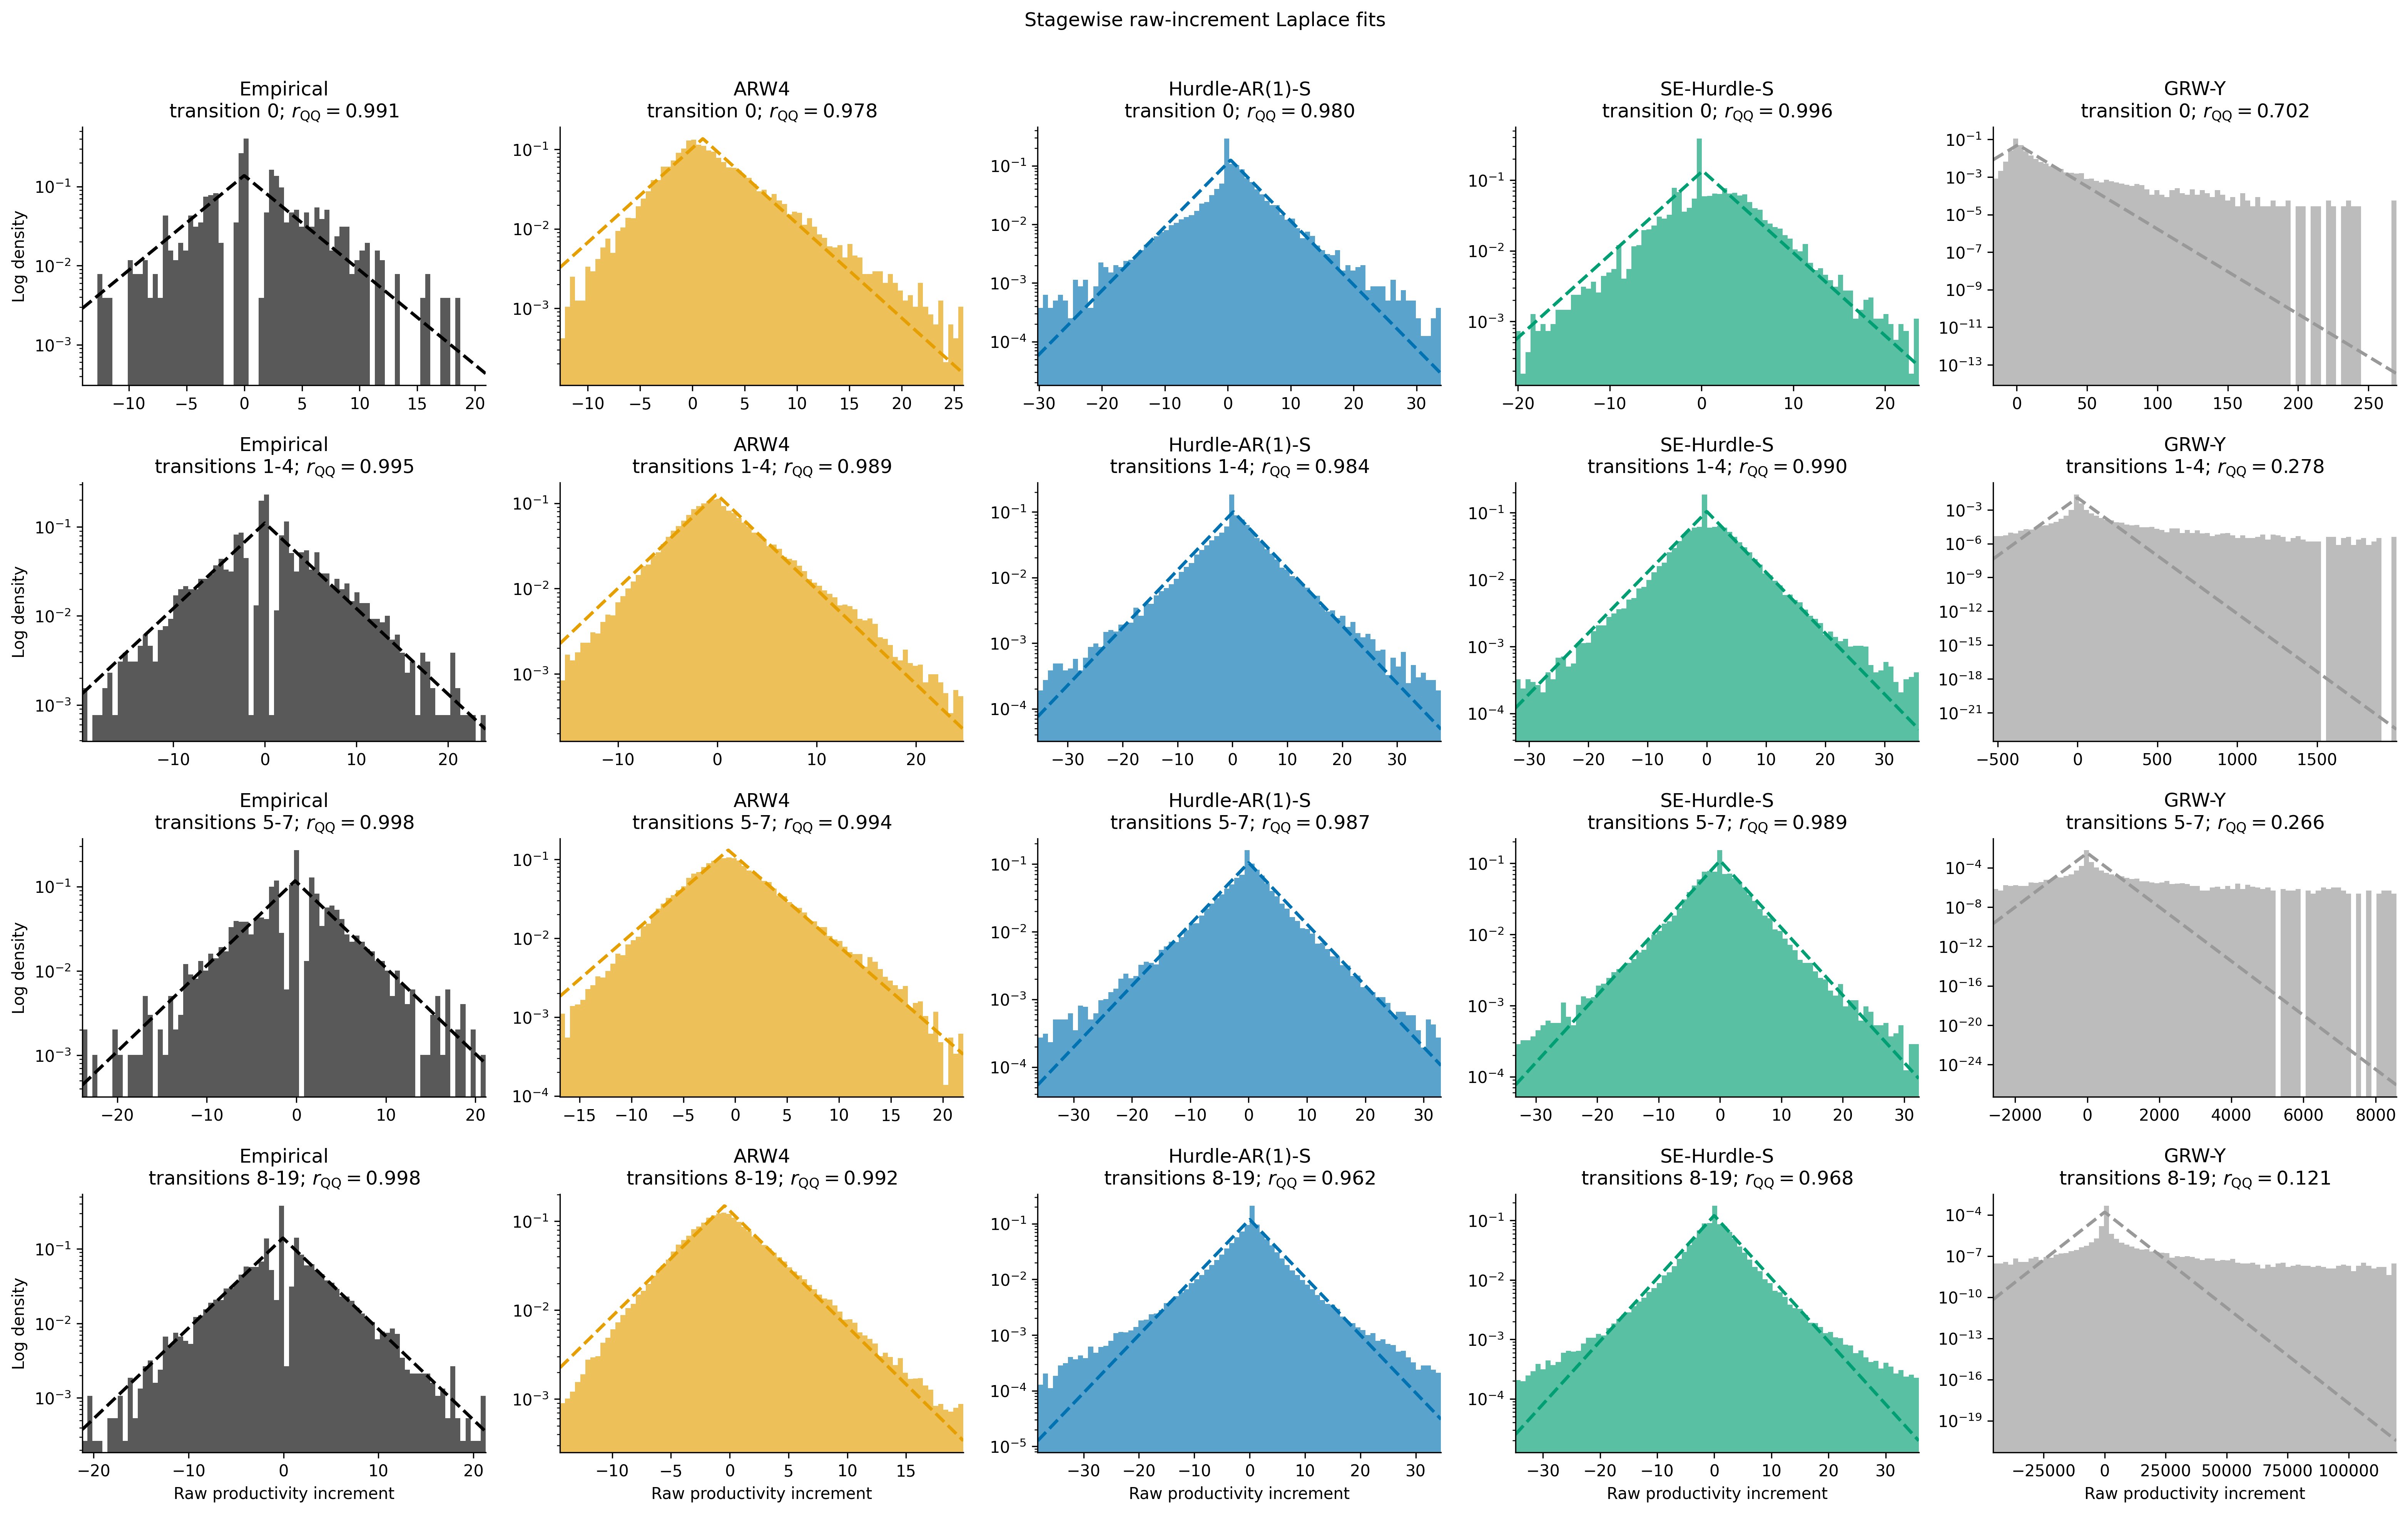
\includegraphics[width=1\linewidth]{figures/raw_increment_laplace_stagewise.png}
    \caption{Fitted Laplace distributions of raw increments across each stage.}
    \label{fig:raw_increment_laplace_stagewise}
\end{figure}

For the purposes of this diagnostic, $r_\text{QQ}$ has been included, but it is important not to rely on that entirely, for reasons discussed in \Cref{results:laplace_distribution}. We see several interesting trends emerge. First, the empirical distribution shows a moat-and-tower shape centered about zero, with a high--- overly high--- point mass at zero and much lower, at times even zero, point mass adjacent to it. 

ARW4 displays the same distribution shape throughout, a sort of right-biased Laplace, as if the distribution had fit but then been incremented counterclockwise about the peak ever so slightly. This systematic underestimatation of negative increments and overestimation of positive increments may warrant further investigation. Of note, it does not reproduce the too-high moat-and-tower signature of the empirical data.

Both hurdle models do reproduce the tower, although not the moat. Hurdle-AR(1)-S maintains a similar shape throughout all stages, which is to say underweight at the center and with excessively heavy tails. This is consistent with \panel{B} and \panel{C} of \Cref{fig:manuscript_marginal_checks}; Hurdle-AR(1)-S shows, over a career, too much density of high variance, which would lead to more increments with a larger magnitude and correspondingly less increments of a smaller magnitude. What is especially exciting is what happens in SE-Hurdle-S. In the first two stages, we saw not quite a moat but certainly a lower point mass immediately about zero while the point mass at zero exceeds the Laplace reference, like empirical; meanwhile, in the rest of the distribution, the tails are far less overestimated. By the third stage and on, it reverts to the same failure mode of Hurdle-AR(1)-S. These results are in line with its marginal distribution of career SD; while it occupies the same failure mode as its autoregressive sister, it does so at a less severe degree. 

GRW-Y's Laplace fit is excluded from the discussion for visible reasons.

\section{Exponential-power increments}
\label{supp:exponential_power_increments}
Having observed a distribution of simulated raw increments more leptokurtic than the usual Laplace, we tested to see what fitting an exponential-power distribution might tell us, which would be HARKing but we're not changing our hypothesis or Laplace diagnostic. We also test the difference between distirbution when excluding zero transitions. We find something notable:

\begin{figure}[H]
    \centering
    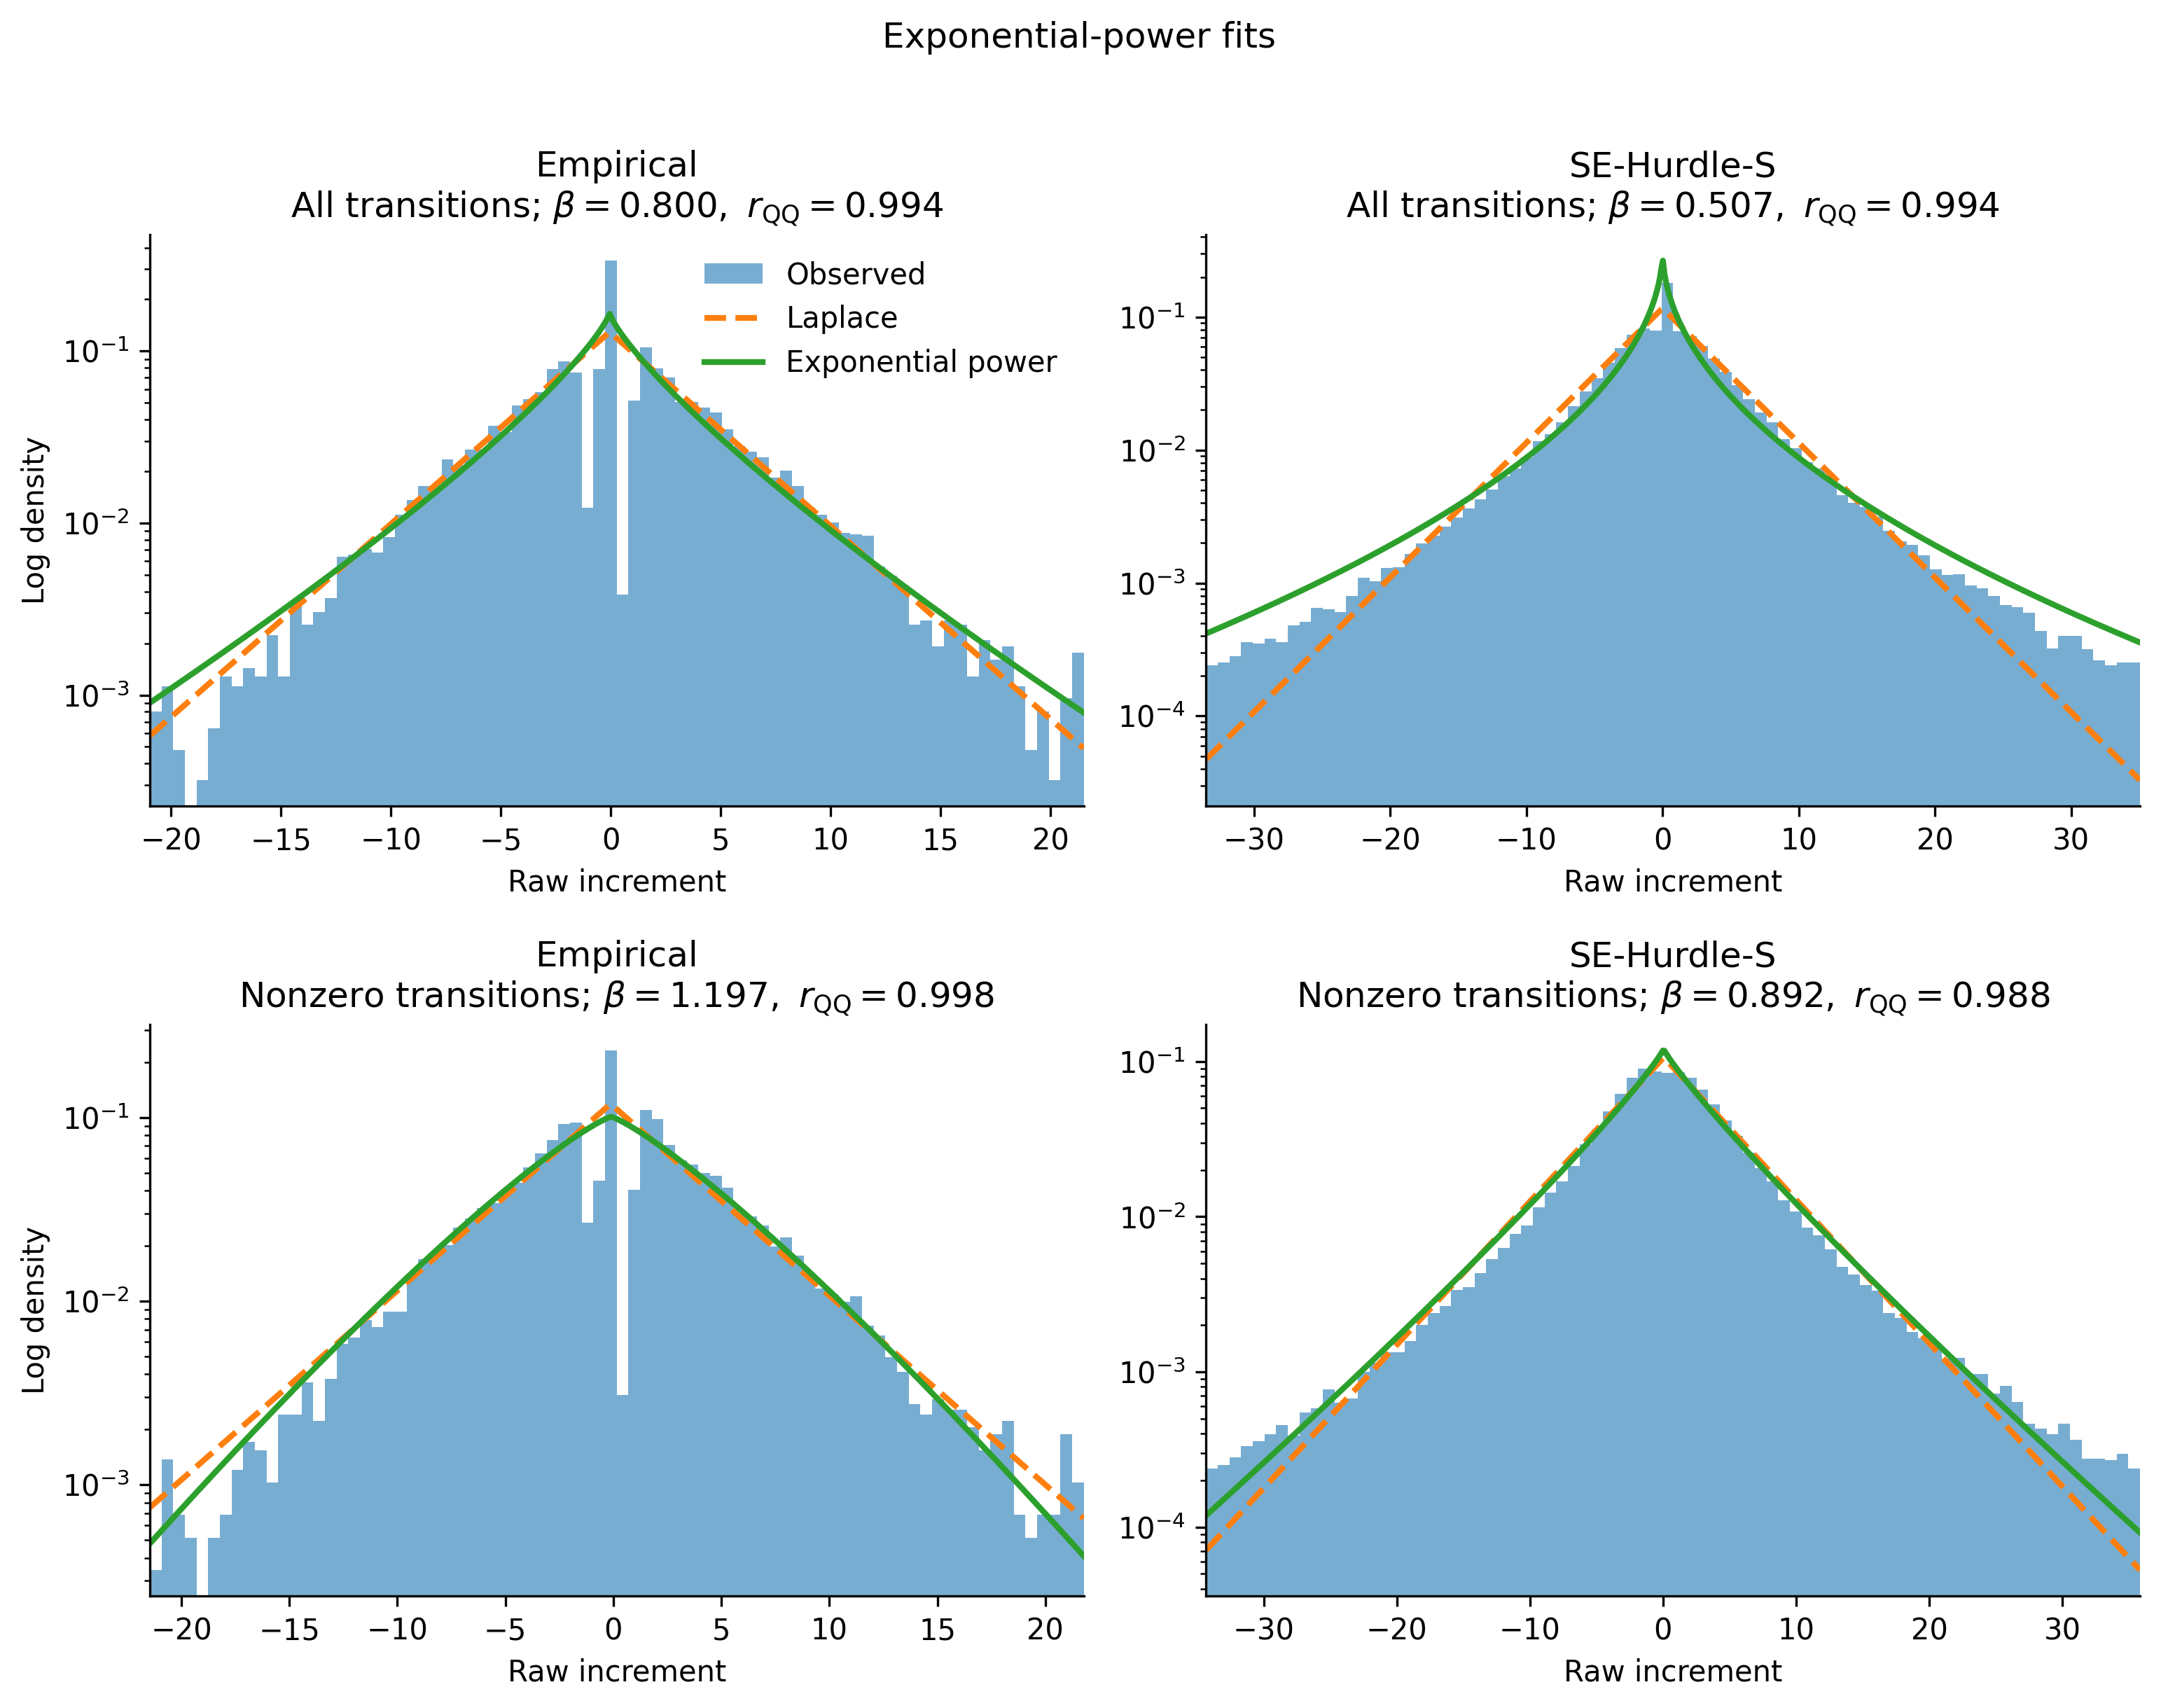
\includegraphics[width=1\linewidth]{figures/raw_increment_exponential_power.png}
    \caption{Histogram of empirical and SE-Hurdle-S raw increments and associated exponential power fits.}
    \label{fig:raw_increment_exponential_power}
\end{figure}

For all empirical increments, $\beta = 0.8< 1$, suggestive of a shorter, sharper, heavier-tailed distribution than Laplace. However, after removing all zero transitions, $\beta = 1.197 > 1$, a shape lying between Laplace and Gaussian, although much closer to Laplace (the special case of exponential power where $\beta = 1$. The empirical marginal distribution, then, is a point mass at zero plus an approximately, but not exactly, Laplace nonzero component. 

In the simulation, however, both all and nonzero increment distributions return $\beta < 1$; the hyper-Laplace shape remains in both cases. The model gets close to Laplace after zero increments are removed, but it does not cross to the empirical side of 1 or match the empirical value. SE-Hurdle-S, then, appears to produce a continuous scale mixture. 

This may suggest a distinct no-change state even outside of consecutive nonpublishing states, reflected in excess mass at 0.

\section{Bugs in the draft code}
\label{supp:bugs}
The geometric random walk in the notebook used for the draft is not fitted over all the empirical data; instead, it is fitted over all nonzero transitions due to a problematic NumPy property in which calling \texttt{np.log} on zeros returns $-\infty$. \texttt{.isfinite} is called after this, leading to the deletion of any transition involving zero. 

\begin{center}
\begin{minipage}{0.85\columnwidth}
\lstinputlisting[
    language=Python
]{code/notebook_blocks_isfinite.py}
\end{minipage}
\end{center}

This means that GRW was fitted only over continuously active transitions, and did not model dropout, restart, or continuous inactivity. 

Further, although Figure 1C of the draft appears to show emergently Laplace-distributed raw increments, this is not the case. 

\begin{figure}[H]
    \centering
    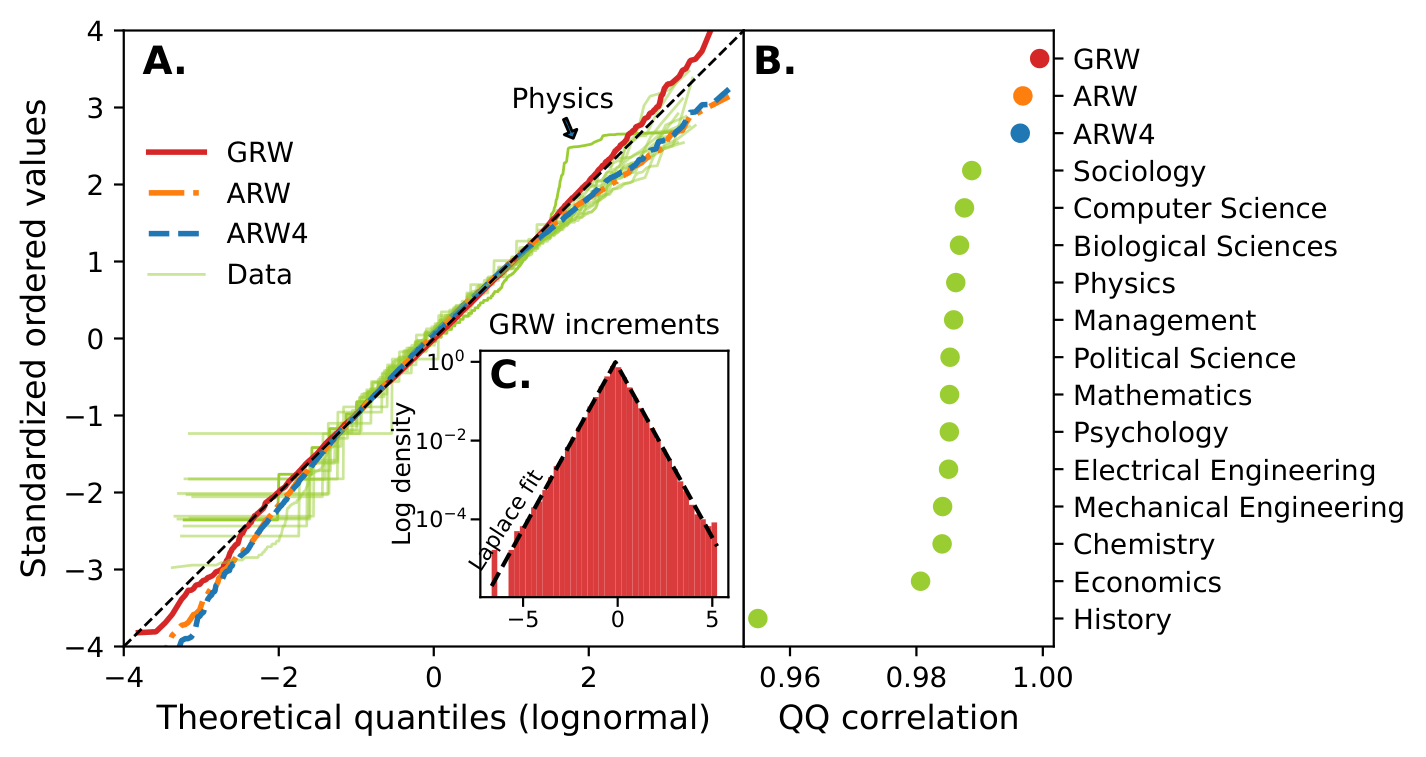
\includegraphics[width=0.75\linewidth]{fig1-1.png}
    \caption{The follow-up draft's QQ diagnostic plot (draft Figure 1); \panel{c} is said to show emergently Laplace-distributed raw increments.}
    \label{fig:draft_fig_1}
\end{figure}

The GRW is run with shocks drawn from \texttt{np.random.laplace()}. Based on the code around this line, (parameters are named \texttt{mu} and \texttt{sigma}, not \texttt{scale} and \texttt{loc}, and there is the addition of a drift correction term frequently used in lognormal processes to counter Jensen's inequality but atypical of Laplace processes), this was unintentional, and \texttt{np.random.normal()} was the intended call. 

\begin{center}
\begin{minipage}{0.85\columnwidth}
\lstinputlisting[
    language=Python
]{code/notebook_block_laplace.py}
\end{minipage}
\end{center}

However, this renders the Laplace distribution structural, rather than emergent. This also raises another issue. According to the draft, the GRW is fitted with parameters $\mu = 0, \sigma^2 = 0.25, x_0 = 4$, and indeed, those values are set in the code (with variance written as $\sigma = 0.5$ instead). However, these parameters are then called in the code with location set as $\mu$ and scale set as $\sigma$. However, for the Laplace distribution, variance is not equal to scale $b$; the relationship is instead $\operatorname{Var}(X) = 2b^2$. The code then computes $Z$ (called \texttt{grw\_logx} in the code). We can compute $\mathbb{E}[Z]$ through linearity of expectation:
\[
\mathbb{E}[Z] = \mathbb{E}[\mu - \frac{\sigma^2}{2}+\epsilon].
\]
The first two terms are constants, so we moved them outside; the \texttt{eps} defined in the code is just a Laplace RV, which is $\mu$, so the whole thing becomes 
\[
\mathbb{E}[Z] = -\frac{\sigma^2}{2}=-0.125, \qquad \operatorname{Var(Z) = 2\sigma^2 = 0.5}.
\]
So while the draft says the parameters are $(\mu = 0, \sigma^2 = 0.25)$, they are in actuality $(\mu = -0.125, \sigma^2 = 0.5)$. On top of that, $\mu$ is called twice, once as the location of \texttt{eps} and then again in the definition of \texttt{grw\_logx}, meaning it is double counted.

Further, in the code, the figure itself is plotted by calling a Laplace fit on \emph{log} increments, not raw, so the outcome is neither emergent nor in correspondence with the findings of the original draft. 

\begin{center}
\begin{minipage}{0.85\columnwidth}
\lstinputlisting[
    language=Python
]{code/notebook_block_log_increments.py}
\end{minipage}
\end{center}

Indeed, when we implemented a GRW in the spirit of the draft (normal draws, all trajectories, no drift correction) we found it did not reproduce Laplace distributions. 

The GRW structure itself is mislabeled and consequently misinterpreted. The draft describes its GRW as 
\[
\begin{aligned}
        & x_2 = x_1\gamma_2\\
        & \hspace{2.4em} x_1 = x_0\gamma_1\\
        & \hspace{4.8em} x_0 = 4,
    \end{aligned} 
\]
or in code form,
\begin{center}
\begin{minipage}{0.85\columnwidth}
\lstinputlisting[
    language=Python
]{code/code_form_of_grw.py}
\end{minipage}
\end{center}

However, in the code, \texttt{eps} is initialized and then immediately cumsummed over all 21 years to get the \texttt{grw\_logx} array, and then exponentiated back to get \texttt{grw\_x}. The problem is, that means \texttt{grw\_x[0]} is actually$x_0\gamma_1 = x_1$, and so on; there's an off-by-one offset. This has wide-ranging implications throughout the draft, and is especially visible in the draft's Figure 2, the rank-mixing diagnostic. According to the caption, that plot shows $\rho(R_0, R_t) \, \forall \; t \in {1,\dots,20}$. Supposing the $x_0 = 4$ condition was actually stored, then every scholar would have the same $x_0$; then, $R_0$ would be tied across the board, with $\operatorname{Var}(R_0) = 0$, making its Spearman correlation with any later year undefined. That, of course, did not happen, showing that the productivity array actually begins with $x_1$.

\begin{figure}[H]
    \centering
    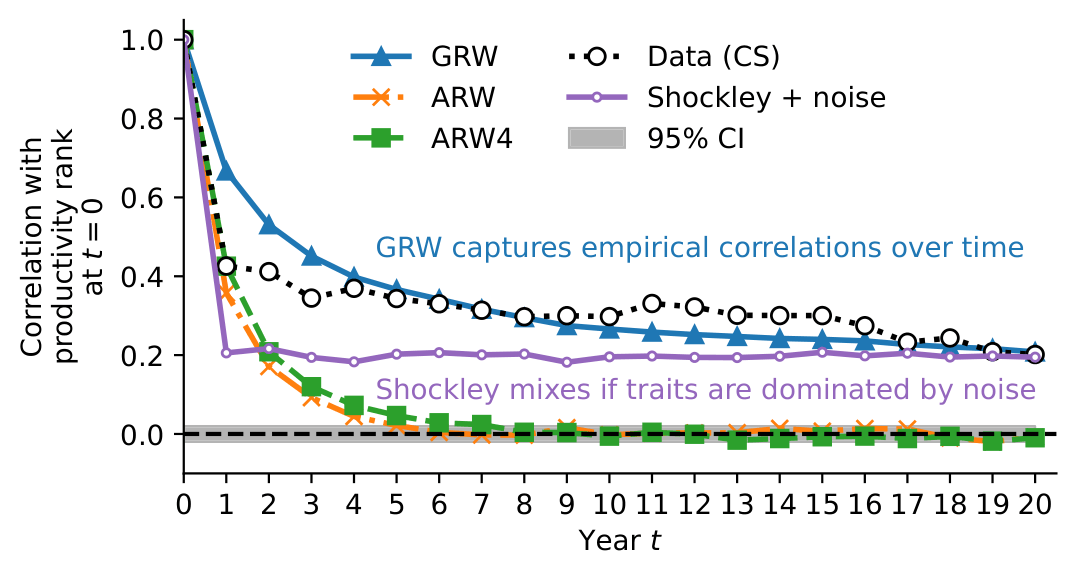
\includegraphics[width=0.75\linewidth]{fig2-1.png}
    \caption{The follow-up draft's rank persistence diagnostic plot (draft Figure 2)}
    \label{fig:draft_fig_2}
\end{figure}

One other bug in the code relates to draft Figure 2 as well. The grey band, described as the 95\% confidence interval for null correlation, is computed as 

\begin{center}
\begin{minipage}{0.85\columnwidth}
\lstinputlisting[
    language=Python
]{code/null_band.py}
\end{minipage}
\end{center}

In all simulation runs, $n = $ 10,000, so the band occupies $\pm 0.0196$. This is fine for the simulation data, all of which have the same sample size, but the empirical data is of $n = 591$; if that quantity was used, the band would occupy $\pm 0.08$, roughly 4 times wider than the current band. So while the band in the draft can answer the question, "If two 10,000 independent rank vectors were unrelated, how far from 0 could observed correlation fluctuate by chance?" it cannot answer anything relating to the empirical data, so no claims can actually be made about the consistency of GRW one way or the other.

\section{Further marginal distributions}
\label{supp:more_marginals}

We appraised SE-Hurdle-S with four additional marginal distributions inherited as diagnostics from the original \textit{Scientific Productivity as a Random Walk}. 

\begin{figure}[H]
    \centering
    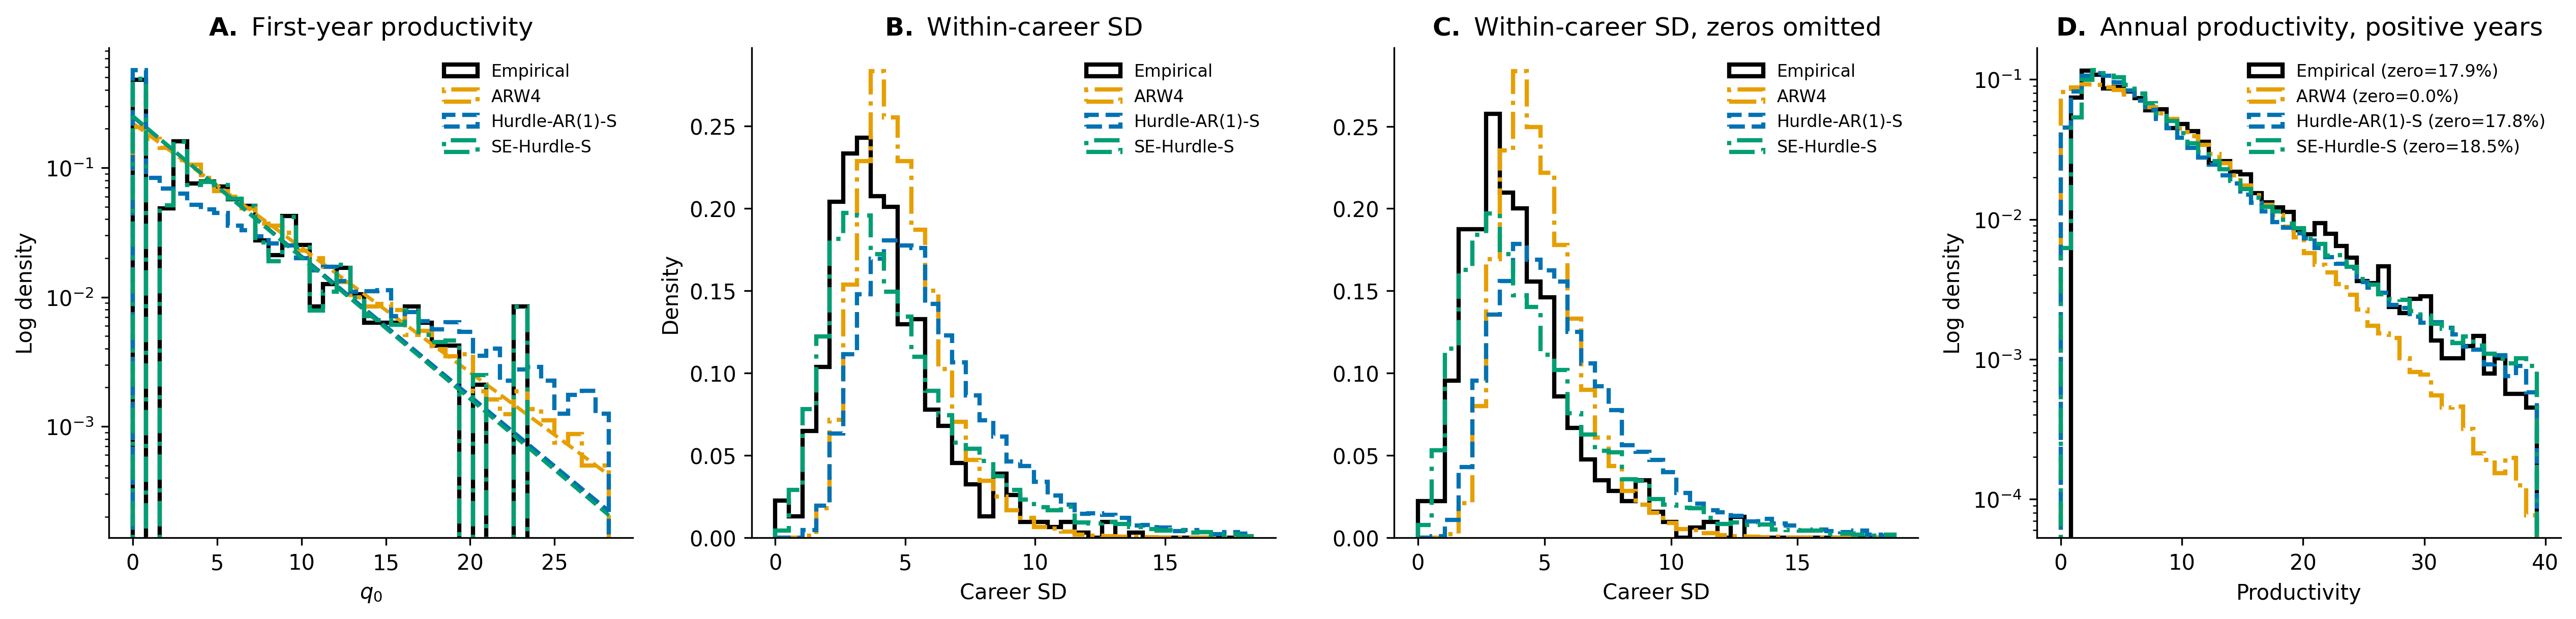
\includegraphics[width=1\linewidth]{figures/manuscript_marginal_checks.png}
    \caption{Four marginal distributions inherited from \textit{SPAARW}. Panel \textbf{A.} describes the log-density of first year productivity against a fitted exponential distribution. Both models do $q_0 \sim \hat{F}_0^{\text{emp}}$, so their replication of the empirical $q_0$ is structurally expected. \textbf{B.} Distribution of $\sigma$ within careers. We retrieve KS $D_{AR(1)} = 0.32, D_{SE} = 0.11$. \textbf{C.} The same, but without zero-years. We retrieve KS $D_{AR(1)} = 0.31, D_{SE} = 0.11$. \textbf{D.} Annual productivity in productive years. Both distributions more strongly resemble each other than the empirical distribution, especially past $q = 20$.}
    \label{fig:manuscript_marginal_checks}
\end{figure}

The first panel sees fairly successful empirical reproduction from Hurdle-AR(1)-S and SE-Hurdle-S because both models initialize their $q_0$ from the empirical distribution; ARW4, meanwhile, returns plausible a distribution with one flaw: no point mass at 0. As discussed just previously, this is a mechanistic shortcoming. 
In \panel{b} and \panel{c}, we assessed the density of careerwise standard deviation with and without zero years considered. The results are broadly identical between the two, suggesting that the mechanistic reasons for them do not involve zero-handling issues. ARW4's marginal distribution is identical between the two because it generates no zeros at all. 

In both instances, the bulk of density is roughly centered about $\sigma \lesssim 4$ in all four distributions; however, both hurdle models underestimate the proportion of density there, maxing out at $\approx 0.20$ while empirical density is $\approx 0.25$, while ARW4 does the opposite, significantly overestimating point mass at the center. Accordingly, both hurdle models overestimate density in the moderate right tail, and ARW4 does the opposite again. Beyond that, however, SE-Hurdle-S outperforms its two cousins; although its mode of reproductive failure is shared with Hurdle-AR(1)-S, the degree of the failure is less pronounced, while ARW4 takes on an opposite failure mode. What is especially notable about this behavior in ARW4 is the earlier observation that it underestimates cross-section variance; this is not contradictory with overestimation of trajectory variance. Rather, it is suggestive of a first-order process that mixes ranks too quickly: scholars do not reliably remain at any intensity over their career. 

In \panel{d}, we observed the comparative log density of annual productivity over all positive years. Interestingly, both hurdle models have a broadly identical distribution, one that loosely overestimates and fails to capture empirical noise beyond $q_t\approx 30$. The modes of failure and success occupied by Hurdle-AR(1)-S and SE-Hurdle-S do not appear to impact the marginal distribution described in \panel{d}. ARW4, meanwhile, severely underestimates log density after around $q_t=20$; this result is highly consistent with its excessively narrow cross-sectional variance. This result overall shows that a model can reproduce the pooled distribution of positive annual productivity while organizing those values incorrectly across scholars and years.

\section{Further lognormality appraisals}
\label{supp:more_lognormal}
We plotted a comparative density histogram of the distribution of log cumulative productivity; in it, we saw highly consistent results from SE-Hurdle-S. 
\begin{figure}[H]
    \centering
    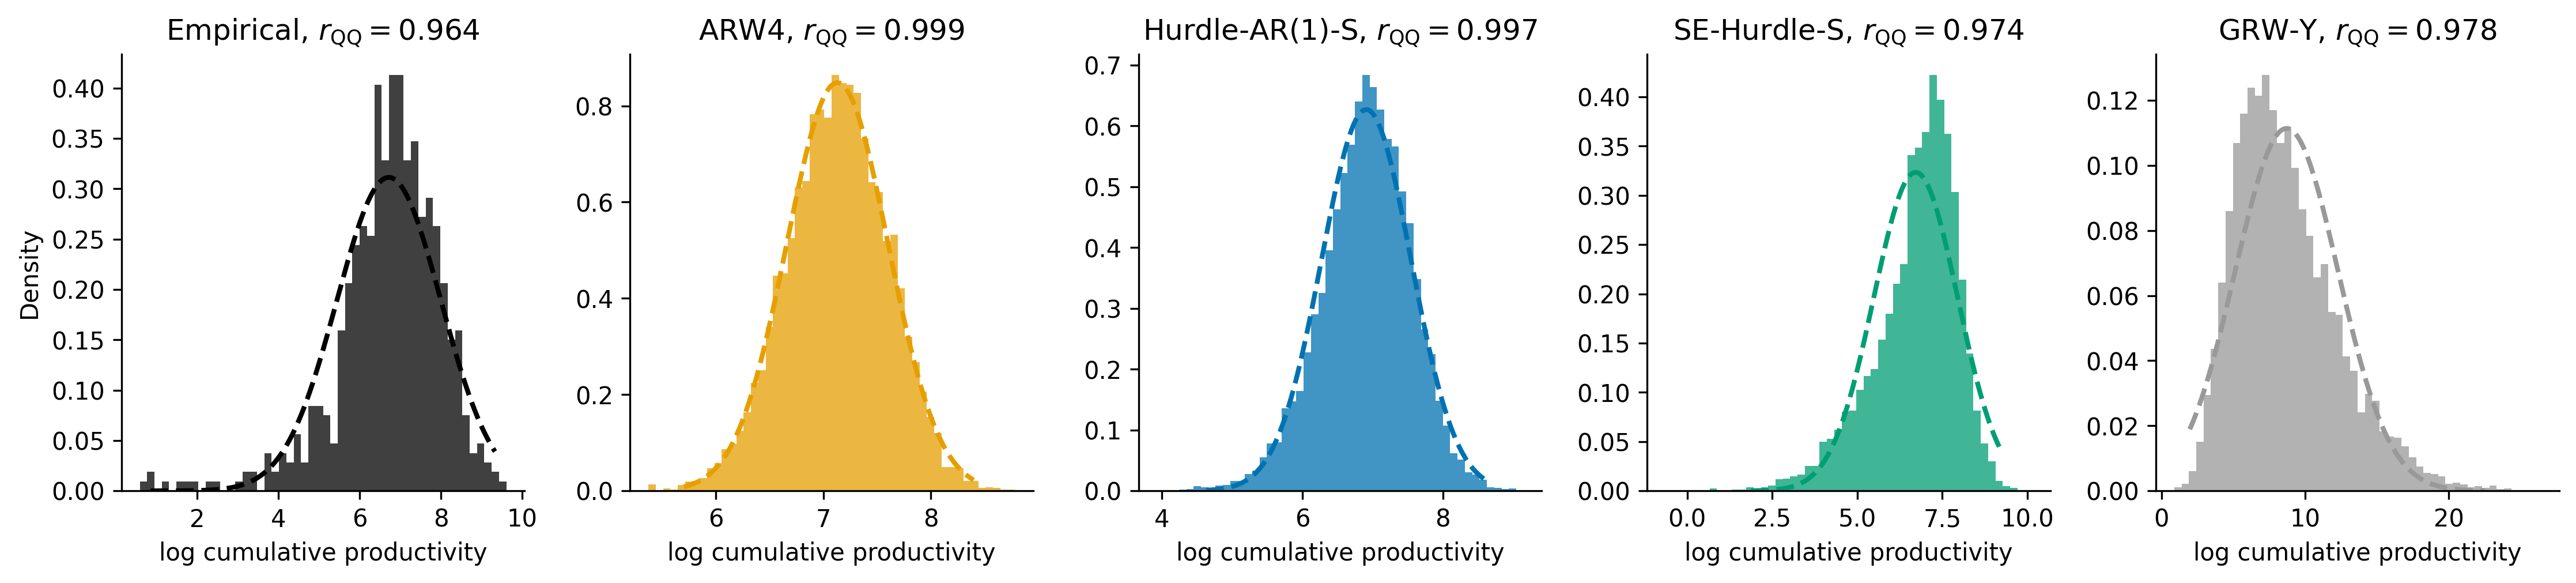
\includegraphics[width=1\linewidth]{figures/cumulative_lognormal.png}
    \caption{Comparative probability distributions of log cumulative productivity.}
    \label{fig:cumulative_lognormal}
\end{figure}
Although Hurdle-AR(1)-S has the best $r_{\text{QQ}}$, it is actually higher than empirical at $\hat{r}_{\text{QQ}} = 0.997$ to $r_{\text{QQ}} = 0.964$, a phenomenon observed throughout lognormal QQ tests. Its QQ is well enclosed under the curve and centered in the same way. However, the empirical data does not match that shape. Rather, the bulk of the mass is at the center-right of the proposed fit, reaching central densities well above the fit. Further, it has a very short right tail and much longer left tail. SE-Hurdle-S is less consistent with a good lognormal fit but it \emph{is} strongly consistent with the empirical distribution: heavy central-right mass, short right tail, long left.

\section{Additional figures}
\label{supp:addl_figs}
The remainder of Supplementary Materials is dedicated to larger subplots for easier viewing of minute detail.

\subsection{Trajectories of moments}
\label{supp:addl_figs_traj_moments}

\paragraph{Mean}

\begin{figure}[H]
    \centering
    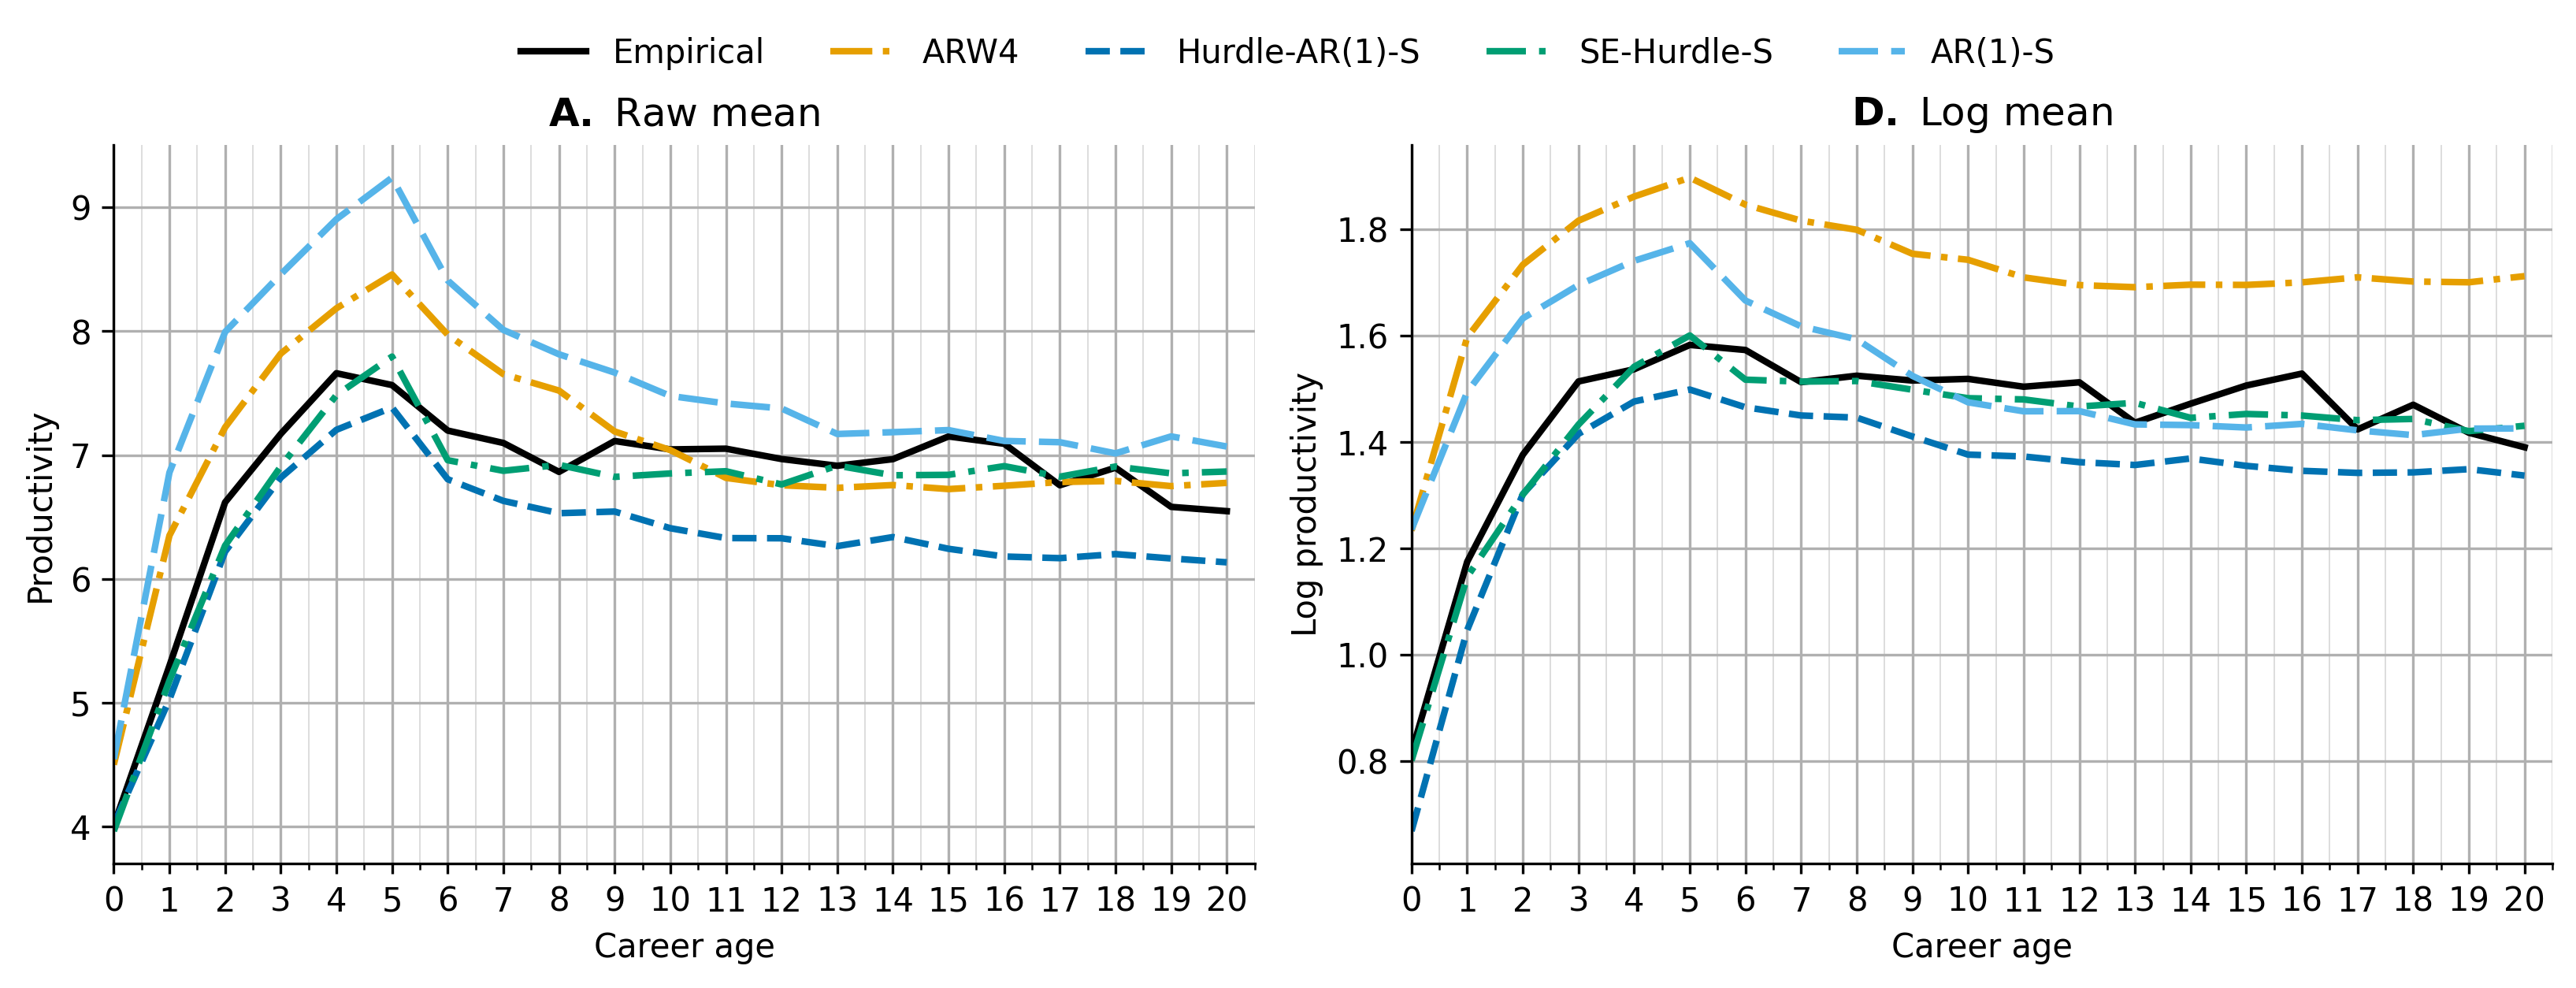
\includegraphics[width=1\linewidth]{figures/mean_trajectories.png}
    \caption{Full-scale view of real and log mean trajectories}
    \label{fig:mean_trajectories}
\end{figure}

\paragraph{Median}

\begin{figure}[H]
    \centering
    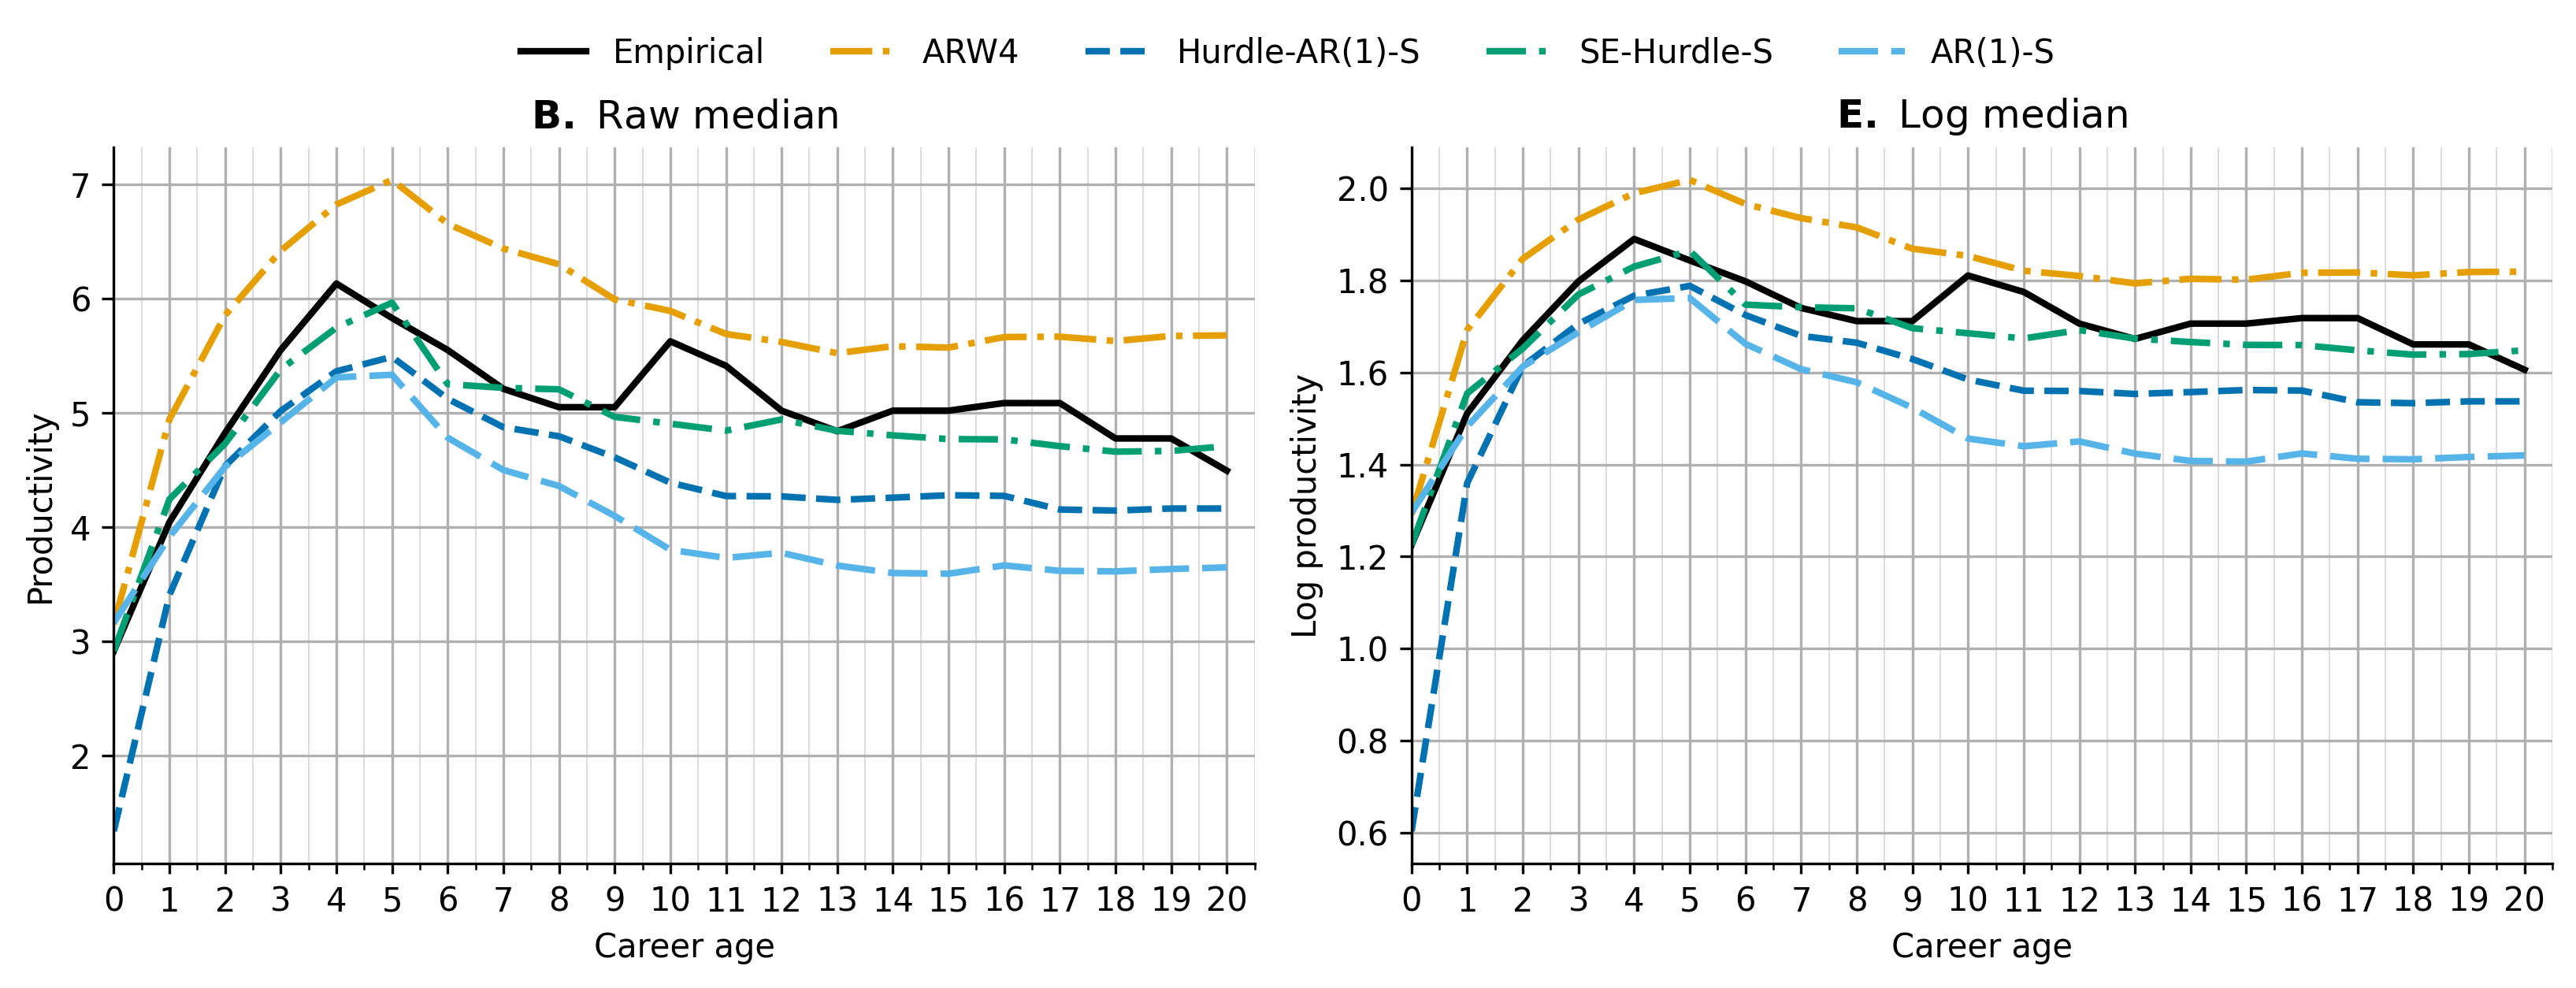
\includegraphics[width=1\linewidth]{figures/median_trajectories.png}
    \caption{Full-scale view of real and log median trajectories.}
    \label{fig:median_trajectories}
\end{figure}

\paragraph{Variance}

\begin{figure}[H]
    \centering
    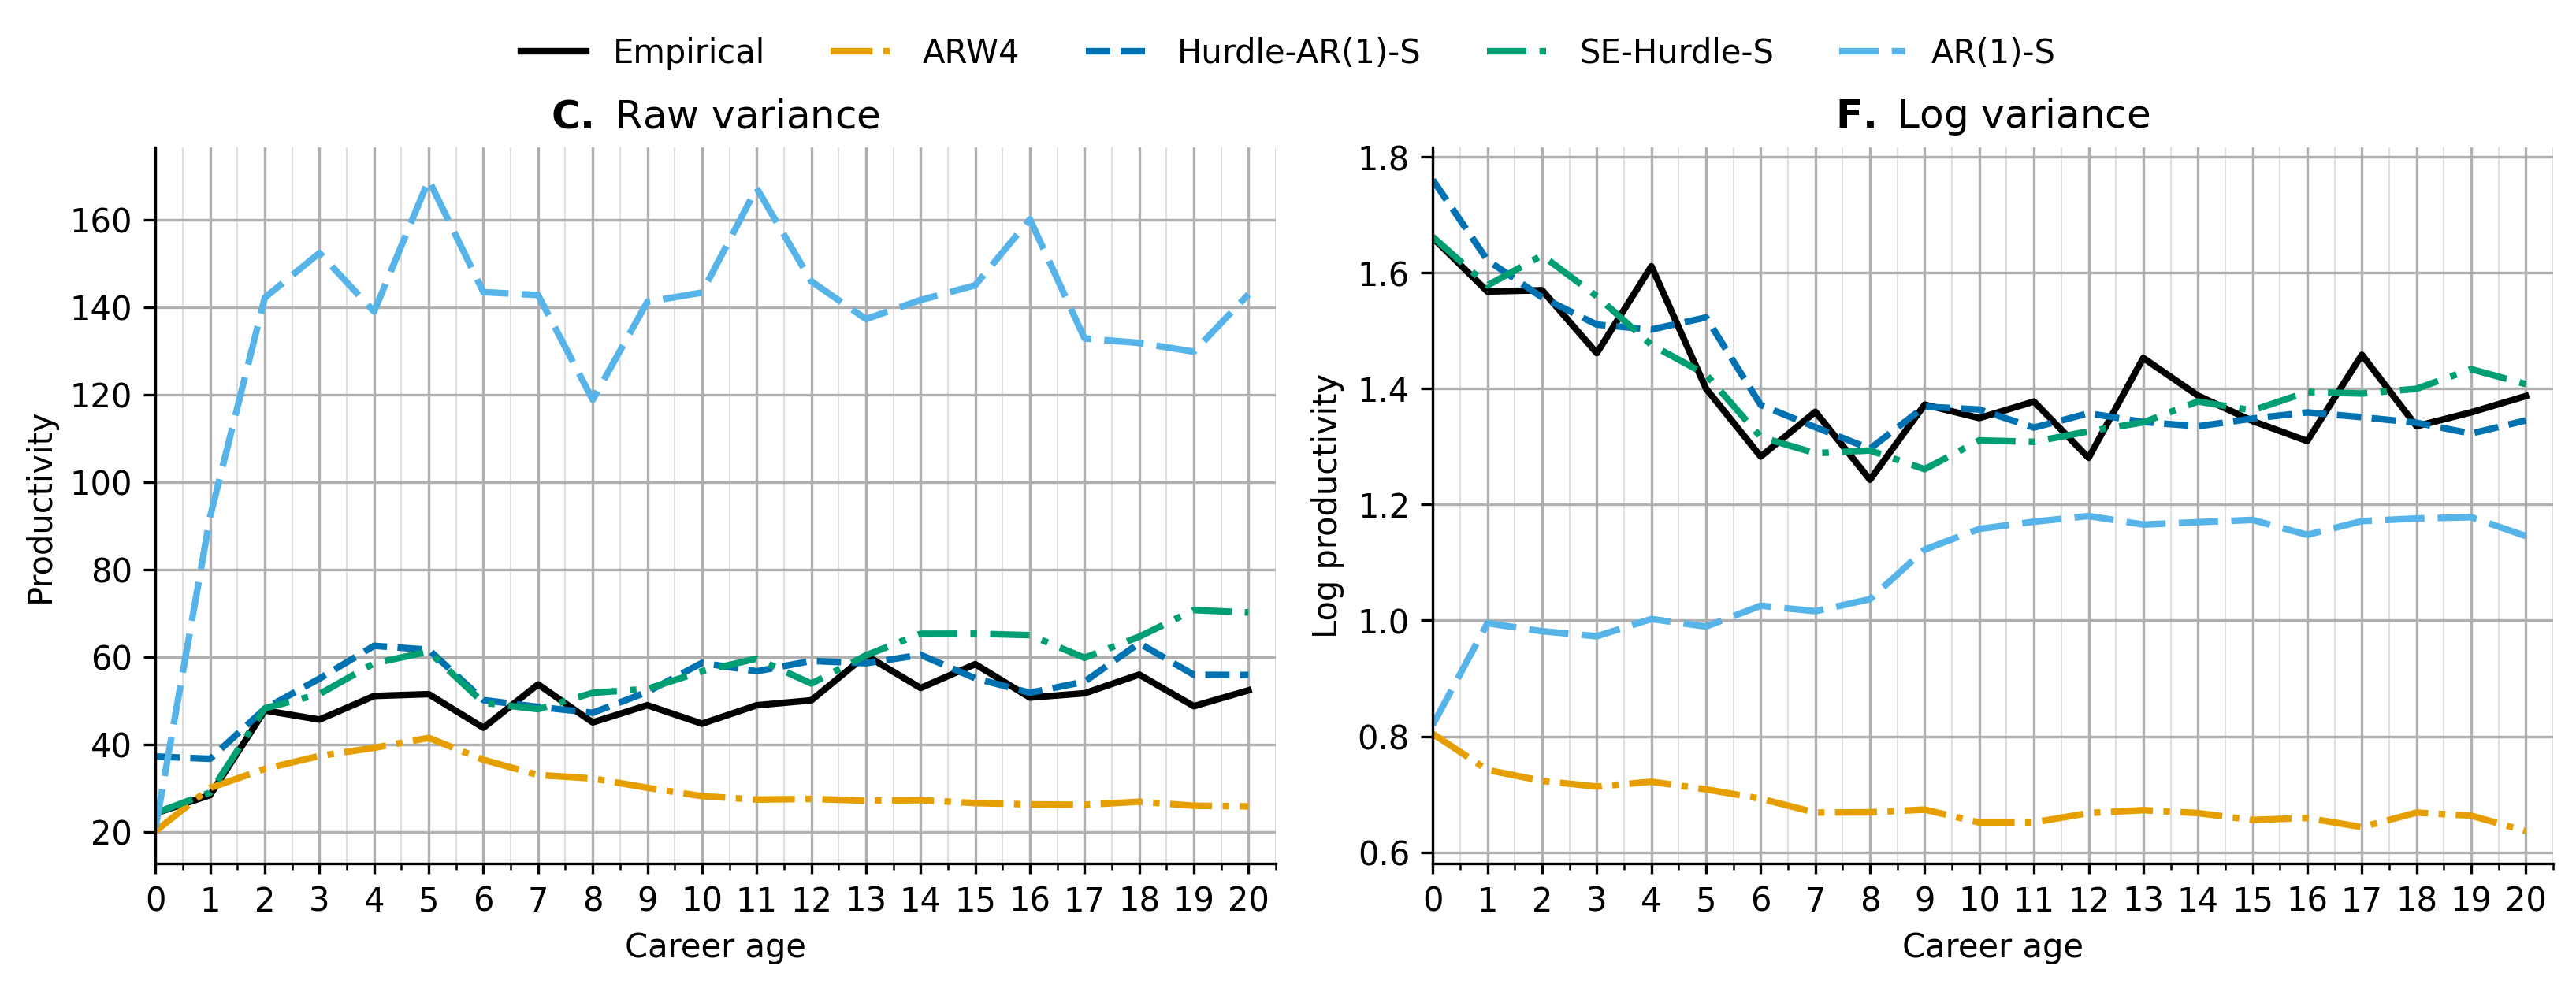
\includegraphics[width=1\linewidth]{figures/variance_trajectories.png}
    \caption{Full-scale view of real and log variance trajectories.}
    \label{fig:variance_trajectories}
\end{figure}

\end{document}